\documentclass[12pt,a4paper]{article}
\usepackage[T1]{fontenc}
\usepackage[polish]{babel}
\usepackage[utf8]{inputenc}
\usepackage{lmodern}
\usepackage{graphicx}
\usepackage{setspace}
\usepackage{geometry}
\geometry{a4paper, margin=2.5cm}
\usepackage{pdfpages}
\usepackage{listings}
\usepackage{xcolor}
\usepackage{float}
\usepackage{subcaption}

\lstdefinelanguage{TypeScript}{
  keywords={import, export, from, async, await, function, return, const, let, type, if, else, for, of, in, new, null, true, false, class, interface, extends, implements},
  keywordstyle=\color{blue}\bfseries,
  ndkeywords={string, number, boolean, Promise, void, any},
  ndkeywordstyle=\color{teal},
  identifierstyle=\color{black},
  sensitive=true,
  comment=[l]{//},
  morecomment=[s]{/*}{*/},
  commentstyle=\color{gray}\ttfamily,
  stringstyle=\color{orange},
  morestring=[b]',
  morestring=[b]",
  morestring=[b]`
}

\lstset{
  language=TypeScript,
  basicstyle=\ttfamily\footnotesize,
  breaklines=true,
  frame=single,
  numbers=left,
  numberstyle=\tiny\color{gray},
  tabsize=2,
  showstringspaces=false
}

\begin{document}

\begin{center}
\textbf{\Large Politechnika Wrocławska}\\[0.3cm]
Wydział Informatyki i Telekomunikacji\\[0.3cm]
Kierunek: IST\\[2cm]

\textbf{\Large ZESPOŁOWE PRZEDSIĘWZIĘCIE INFORMATYCZNE}\\[2cm]

\textbf{\Large AI Present Finder}\\[2cm]

Dawid Chudzicki\\[0.2cm]
Marcin Dolatowski\\[0.2cm]
Bartosz Gotowski\\[0.2cm]
Szymon Kowaliński\\[2cm]

Opiekun pracy\\
dr inż. Marcin Jodłowiec\\[2cm]


WROCŁAW 2025
\end{center}

\newpage

\tableofcontents
\newpage

\section*{DOKUMENTACJA PROJEKTOWA}
\addcontentsline{toc}{section}{DOKUMENTACJA PROJEKTOWA}

\section{Wykaz symboli, oznaczeń i akronimów (opcja)}

\begin{tabular}{|p{0.15\textwidth}|p{0.3\textwidth}|p{0.45\textwidth}|}
\hline
\textbf{Skrót} & \textbf{Pełna nazwa} & \textbf{Opis} \\
\hline
AI & Artificial Intelligence & Sztuczna inteligencja – technologia wykorzystująca algorytmy uczenia maszynowego. \\
\hline
API & Application Programming Interface & Interfejs programistyczny umożliwiający komunikację między systemami. \\
\hline
UI & User Interface & Interfejs użytkownika. \\
\hline
UX & User Experience & Doświadczenie użytkownika. \\
\hline
VPS & Virtual Private Server & Wirtualny serwer prywatny. \\
\hline
OSINT & Open Source Intelligence & Biały wywiad, pozyskiwanie informacji z ogólnodostępnych źródeł. \\
\hline
LLM & Large Language Model & Duży model językowy (np. GPT-4, Gemini). \\
\hline
SSE & Server-Sent Events & Technologia przesyłania aktualizacji z serwera do klienta. \\
\hline
CQRS & Command Query Responsibility Segregation & Wzorzec architektoniczny rozdzielający odczyt od zapisu. \\
\hline
\end{tabular}

\section{Cel i zakres przedsięwzięcia}

\subsection{Wstęp}
Celem projektu jest opracowanie aplikacji webowej do proponowania spersonalizowanych prezentów dla osób na podstawie podanych linków do ich mediów społecznościowych, a także podanych zainteresowań i cech podczas wywiadu z chatbotem. Na podstawie danych system generuje przykładowe propozycje prezentów, aby następnie wyszukać je w zintegrowanych serwisach sklepowych i zwrócić linki do ofert użytkownikowi.

\subsection{Cel główny}
Stworzenie użytecznego, szybkiego i bezpiecznego narzędzia wspierającego proces znajdowania prezentu poprzez:
\begin{itemize}
    \item automatyczne wydobycie i analizę cech osoby na podstawie mediów społecznościowych (OSINT),
    \item interaktywny chat z agentem AI w celu zebrania dodatkowych informacji,
    \item generowanie trafnych propozycji prezentów na podstawie uzyskanych danych,
    \item proponowanie konkretnych ofert produktów ze sklepów internetowych (agregacja).
\end{itemize}

\subsection{Zakres projektu}
\textbf{Co wchodzi w zakres projektu:}
\begin{itemize}
    \item interfejs webowy do wprowadzania linków do publicznych profili społecznościowych i prowadzenia chatu z użytkownikiem,
    \item moduł parsowania i ekstrakcji jedynie publicznych, jawnych danych z podanych profili,
    \item generowanie propozycji prezentów dla wybranej osoby,
    \item propozycja ofert prezentów ze sklepów internetowych (OLX, Allegro, eBay, Amazon),
    \item filtry wyników (np. po cenie, kategorii).
\end{itemize}

\textbf{Co nie wchodzi w zakres projektu:}
\begin{itemize}
    \item automatyczne dokonywanie zakupów ani płatności,
    \item zbieranie prywatnych danych wymagających logowania,
    \item integracja OAuth z zewnętrznymi kontami użytkownika,
    \item generowanie treści graficznych produktów (korzystamy z gotowych zdjęć ofert).
\end{itemize}

\subsection{Cele biznesowe i techniczne}
Z biznesowego punktu widzenia projekt ma na celu skrócenie czasu potrzebnego na znalezienie prezentu z kilkunastu godzin do kilku minut oraz zwiększenie trafności upominków. Z technicznego punktu widzenia celem jest weryfikacja możliwości wykorzystania modeli LLM do sterowania procesem wyszukiwania i selekcji ofert (Agentic Commerce) oraz integracja wielu źródeł danych w czasie rzeczywistym.

\section{Słownik pojęć (opcja)}

\begin{tabular}{|p{0.25\textwidth}|p{0.7\textwidth}|}
\hline
\textbf{Pojęcie} & \textbf{Opis / Definicja} \\
\hline
AI Present Finder & Nazwa projektu — aplikacja webowa wykorzystująca sztuczną inteligencję do proponowania spersonalizowanych prezentów. \\
\hline
Użytkownik & Osoba korzystająca z aplikacji w celu znalezienia pomysłu na prezent dla innej osoby. \\
\hline
Osoba obdarowywana & Osoba, której profil jest analizowany przez system w celu znalezienia prezentu. \\
\hline
Chatbot / Agent AI & Moduł oparty na LLM prowadzący rozmowę z użytkownikiem, zadający pytania o preferencje, okazję i budżet. \\
\hline
Profil społecznościowy & Publicznie dostępna strona użytkownika w mediach społecznościowych (np. Instagram, TikTok). \\
\hline
Ekstrakcja danych & Proces automatycznego pobierania i analizy publicznych informacji z profili. \\
\hline
Propozycja prezentu & Wygenerowany przez AI ogólny pomysł na prezent (np. "Aparat analogowy"). \\
\hline
Propozycja oferty & Konkretny link do produktu w sklepie internetowym (np. aukcja na Allegro). \\
\hline
Filtrowanie wyników & Zawężanie listy rekomendacji według kryteriów takich jak cena czy kategoria. \\
\hline
Dane publiczne & Ogólnodostępne informacje w Internecie, niewymagające logowania ani specjalnych uprawnień do odczytu. \\
\hline
\end{tabular}

\section{Stan wiedzy w obszarze przedsięwzięcia (opcja)}

Rynek cyfrowego wsparcia w obdarowywaniu można podzielić na dwa główne segmenty: rozwiązania B2B (Corporate Gifting) oraz B2C (Consumer Chatbots). Rozwiązania B2B (np. Giftpack.ai) oferują wysoką jakość dzięki analizie danych, ale są niedostępne dla klienta indywidualnego. Rozwiązania B2C (np. DreamGift) są łatwo dostępne, ale często opierają się na prostych chatbotach bez kontekstu, co prowadzi do niskiej trafności rekomendacji.

Poniższa tabela przedstawia porównanie AI Present Finder z istniejącymi rozwiązaniami konsumenckimi:

\begin{table}[h]
\centering
\begin{tabular}{|p{0.2\textwidth}|p{0.2\textwidth}|p{0.2\textwidth}|p{0.15\textwidth}|p{0.15\textwidth}|}
\hline
\textbf{Rozwiązanie} & \textbf{Źródła danych} & \textbf{Interakcja} & \textbf{Dokładność} & \textbf{Integracja e-commerce} \\
\hline
\textbf{AI Present Finder} & \textbf{Media społecznościowe + chatbot} & \textbf{Szczegółowy wywiad (ok. 20 pytań)} & \textbf{Wysoka} & \textbf{OLX, Amazon, eBay, Allegro} \\
\hline
DreamGift & Tylko rozmowa & Krótka (ok. 6 pytań) & Niska/ogólna & Amazon \\
\hline
GiftAssistant & 3 pola tekstowe & Brak konwersacji & Niska (4 propozycje) & Amazon \\
\hline
Giftruly & Formularz & Kilka pól wyboru & Podstawowa & Amazon \\
\hline
IntelliGift & Pola tekstowe & Szerokie dane & Średnia & Amazon \\
\hline
\end{tabular}
\caption{Porównanie rozwiązań rynkowych}
\end{table}

Głównym wyróżnikiem AI Present Finder jest połączenie analizy OSINT (rozwiązującej problem "zimnego startu") z lokalną agregacją ofert (OLX, Allegro), co pozwala na znajdowanie unikatowych prezentów niedostępnych w globalnych katalogach typu Amazon.

\section{Założenia wstępne}

\subsection{Założenia technologiczne}
\begin{itemize}
    \item \textbf{Frontend:} React (Single Page Application)
    \item \textbf{Backend:} NestJS (Node.js framework)
    \item \textbf{Baza danych:} PostgreSQL
    \item \textbf{Komunikacja:} RabbitMQ (kolejkowanie zadań), REST API, SSE
    \item \textbf{Integracje zewnętrzne:}
    \begin{itemize}
        \item API mediów społecznościowych (poprzez proxy/scraping)
        \item API e-commerce: OLX, Amazon, eBay, Allegro Sandbox
        \item OpenAI API / Google Gemini API (modele językowe)
    \end{itemize}
    \item \textbf{Hosting:} VPS, obsługa HTTPS
\end{itemize}

\subsection{Założenia projektowe i ograniczenia}
\begin{itemize}
    \item Przetwarzane są wyłącznie dane publicznie dostępne (OSINT).
    \item System nie obsługuje płatności ani finalizacji transakcji (przekierowanie do sklepu).
    \item Dane osobowe nie są trwale przechowywane po zakończeniu sesji użytkownika.
    \item Projekt ma charakter edukacyjno-prototypowy (MVP).
\end{itemize}

\section{Analiza wymagań i sposób pracy}

Projekt był realizowany iteracyjnie w podejściu zbliżonym do Agile. Zespół korzystał z GitHub Issues jako backlogu produktu, dzieląc prace na kolejne iteracje (POC, Design, MVP, Deploy). Każdy issue reprezentował konkretne wymaganie lub zadanie, a kolumny statusu (Backlog / Todo / Done) odzwierciedlały postęp prac. Przebieg projektu przedstawiono na Rysunku~\ref{fig:iteration-timeline}.

\begin{figure}[H]
    \centering
    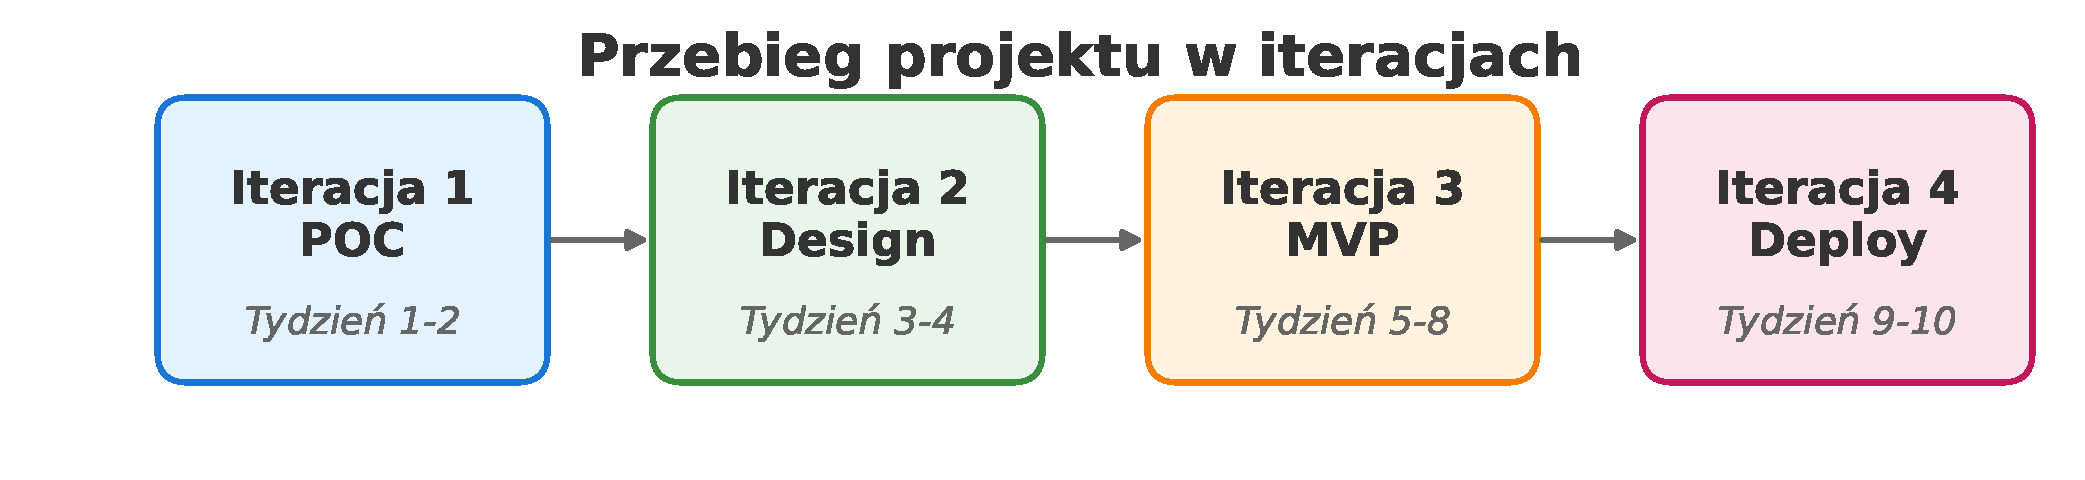
\includegraphics[width=\textwidth]{iteration_timeline.pdf}
    \caption{Przebieg projektu w czterech iteracjach.}
    \label{fig:iteration-timeline}
\end{figure}

\subsection{Iteracja 1: POC (Proof of Concept)}
Celem pierwszej iteracji było sprawdzenie, czy kluczowe ryzyka technologiczne są rozwiązywalne:
\begin{itemize}
    \item przygotowanie \textbf{NestJS boilerplate} z obsługą zdarzeń (issue: \textit{"NestJS boilerplate z zmockowanymi eventami"}),
    \item \textbf{Gift Search POC} – przetestowanie możliwości wyszukiwania prezentów w zewnętrznych serwisach,
    \item \textbf{POC scrapera Facebooka, Instagrama i Tiktoka} – weryfikacja, czy da się zbudować moduł OSINT,
    \item uruchomienie podstawowego \textbf{frontendu} ("set up basic frontend project"),
    \item przygotowanie pierwszych \textbf{diagramów}: C4, BPMN, projekt premise.
\end{itemize}
Rezultatem iteracji POC było potwierdzenie, że analiza profili, komunikacja zdarzeniowa i podstawowe wyszukiwanie produktów są możliwe w przyjętym stosie technologicznym. Na tym etapie powstały również pierwsze makiety interfejsu (Figma) oraz wstępny podział odpowiedzialności w zespole (backend, frontend, DevOps).

\subsection{Iteracja 2: Design}
Druga iteracja skupiła się na doprecyzowaniu architektury i modelu domeny:
\begin{itemize}
    \item utworzenie \textbf{diagramów C4} (wersja ogólna i wersja mikroserwisowa),
    \item przygotowanie \textbf{diagramu klas} oraz \textbf{diagramu BPMN} opisującego przepływ procesu,
    \item doprecyzowanie podziału na mikroserwisy i kontraktów między nimi,
    \item konfiguracja środowiska developerskiego i CI.
\end{itemize}
Na koniec iteracji Design powstał spójny model architektoniczny, który został wykorzystany przy budowie MVP.

\subsection{Iteracja 3: MVP}
Trzecia iteracja miała na celu dostarczenie \textbf{działającego MVP} aplikacji:
\begin{itemize}
    \item wyodrębnienie mikroserwisów: \textit{gift-ideas-microservice}, \textit{reranking-microservice}, \textit{fetch-microservice},
    \item integracja chatu z architekturą zdarzeniową ("EPIC: integrate chat POC with microservices setup"),
    \item dodanie widoków \textbf{frontendowych}: home, stalking, chat, rekomendacje,
    \item implementacja \textbf{historii czatu} oraz \textbf{historii rekomendacji prezentów},
    \item dodanie \textbf{ulubionych produktów}, filtrowania i sortowania,
    \item pierwsza wersja \textbf{systemu rerankingu} i integracja z platformami e-commerce.
\end{itemize}
W trakcie iteracji MVP powstał też \textbf{landing page} oraz logotyp projektu. Celem biznesowym było udostępnienie wersji, która rozwiązuje podstawowy problem użytkownika: wygenerowanie sensownych propozycji prezentów w jednym miejscu.

Przykładowo, podczas jednego z wewnętrznych testów MVP okazało się, że standardowe wyszukiwanie produktów zwraca wiele duplikatów oraz ofert zupełnie niepasujących do profilu obdarowywanej osoby (np. części zamienne zamiast gotowych prezentów). To konkretne doświadczenie doprowadziło do zaprojektowania dedykowanego modułu rerankingu opartego na AI, który odfiltrowuje szum i eksponuje najbardziej trafne propozycje.

\subsection{Iteracja 4: Deploy}
Ostatnia iteracja skupiła się na przygotowaniu systemu do beta-testów i wdrożenia produkcyjnego:
\begin{itemize}
    \item dodanie \textbf{logowania i autoryzacji} (Google OAuth, uprawnienia, odświeżanie tokenów),
    \item rozbudowa \textbf{panelu użytkownika} oraz \textbf{panelu administratora},
    \item dopracowanie \textbf{UX/UI} (animacje chatu, lepszy layout na desktopie, landing page),
    \item optymalizacje \textbf{rerankingu} (usuwanie duplikatów, pararelizacja oceniania, pętla regeneracji propozycji),
    \item \textbf{tłumaczenie} aplikacji na język polski,
    \item przygotowanie \textbf{deploymentu} (CI/CD, migracje bazy danych, health-checki).
\end{itemize}
W tej iteracji skoncentrowano się również na przygotowaniu aplikacji do testów z realnymi użytkownikami oraz zbieraniu feedbacku (gwiazdki, formularze opinii). Pojawiły się też mechanizmy refinementu (dopytywanie o lepsze prezenty na podstawie wcześniejszych wyborów) oraz pytanie o budżet przed rozpoczęciem wywiadu.

Na podstawie tak zebranych i iteracyjnie doprecyzowywanych wymagań przygotowano poniższą specyfikację produktu programowego.

\subsection{Organizacja pracy zespołu}
Zespół pracował w składzie czteroosobowym, z wyraźnym podziałem ról:
\begin{itemize}
    \item Dawid Chudzicki – lider backendu i Project Manager, odpowiedzialny za architekturę (C4, diagramy sekwencji), logikę rdzeniową oraz moduł autentykacji (Google OAuth).
    \item Marcin Dolatowski – odpowiedzialny za integracje zewnętrzne (fetch-microservice, sklepy), Reranking Microservice oraz refaktoryzację i dopracowanie interfejsu użytkownika (landing page, UI).
    \item Bartosz Gotowski – DevOps i infrastruktura (Coolify, Docker, CI/CD, migracje bazy danych), monitoring oraz dokumentacja techniczna (LaTeX, diagramy C4/BPMN).
    \item Szymon Kowaliński – architektura mikroserwisów, implementacja SSE, logika chatu (gotowe odpowiedzi), poprawki i optymalizacje na styku frontend–backend.
\end{itemize}
Postęp prac był regularnie raportowany prowadzącemu w formie statusów (co kto aktualnie robi, jaki jest plan na sprint i jakie pojawiły się ryzyka), co ułatwiało korygowanie zakresu MVP oraz planowanie kolejnych iteracji (m.in. sprint poświęcony testom i optymalizacji aplikacji).

\subsection{Przypadki użycia}
Na podstawie zebranych wymagań zdefiniowano kluczowe przypadki użycia (Use Case), m.in.:
\begin{itemize}
    \item U1: Użytkownik podaje linki do profili społecznościowych osoby obdarowywanej.
    \item U2: Użytkownik przeprowadza wywiad z chatbotem (okazja, budżet, preferencje).
    \item U3: System analizuje dane (OSINT + wywiad) i generuje listę pomysłów na prezenty.
    \item U4: System wyszukuje i prezentuje oferty produktów z wielu sklepów.
    \item U5: Użytkownik filtruje i sortuje wyniki, dodaje produkty do ulubionych i historii.
    \item U6: Administrator przegląda statystyki i zarządza użytkownikami (panel admina).
\end{itemize}

Graficzna reprezentacja tych przypadków została przygotowana w postaci diagramu przypadków użycia UML (Rysunek~\ref{fig:use-case}), gdzie aktorami są m.in. \textit{Użytkownik}, \textit{Administrator} oraz zewnętrzne systemy (sklepy, media społecznościowe).

\begin{figure}[ht]
    \centering
    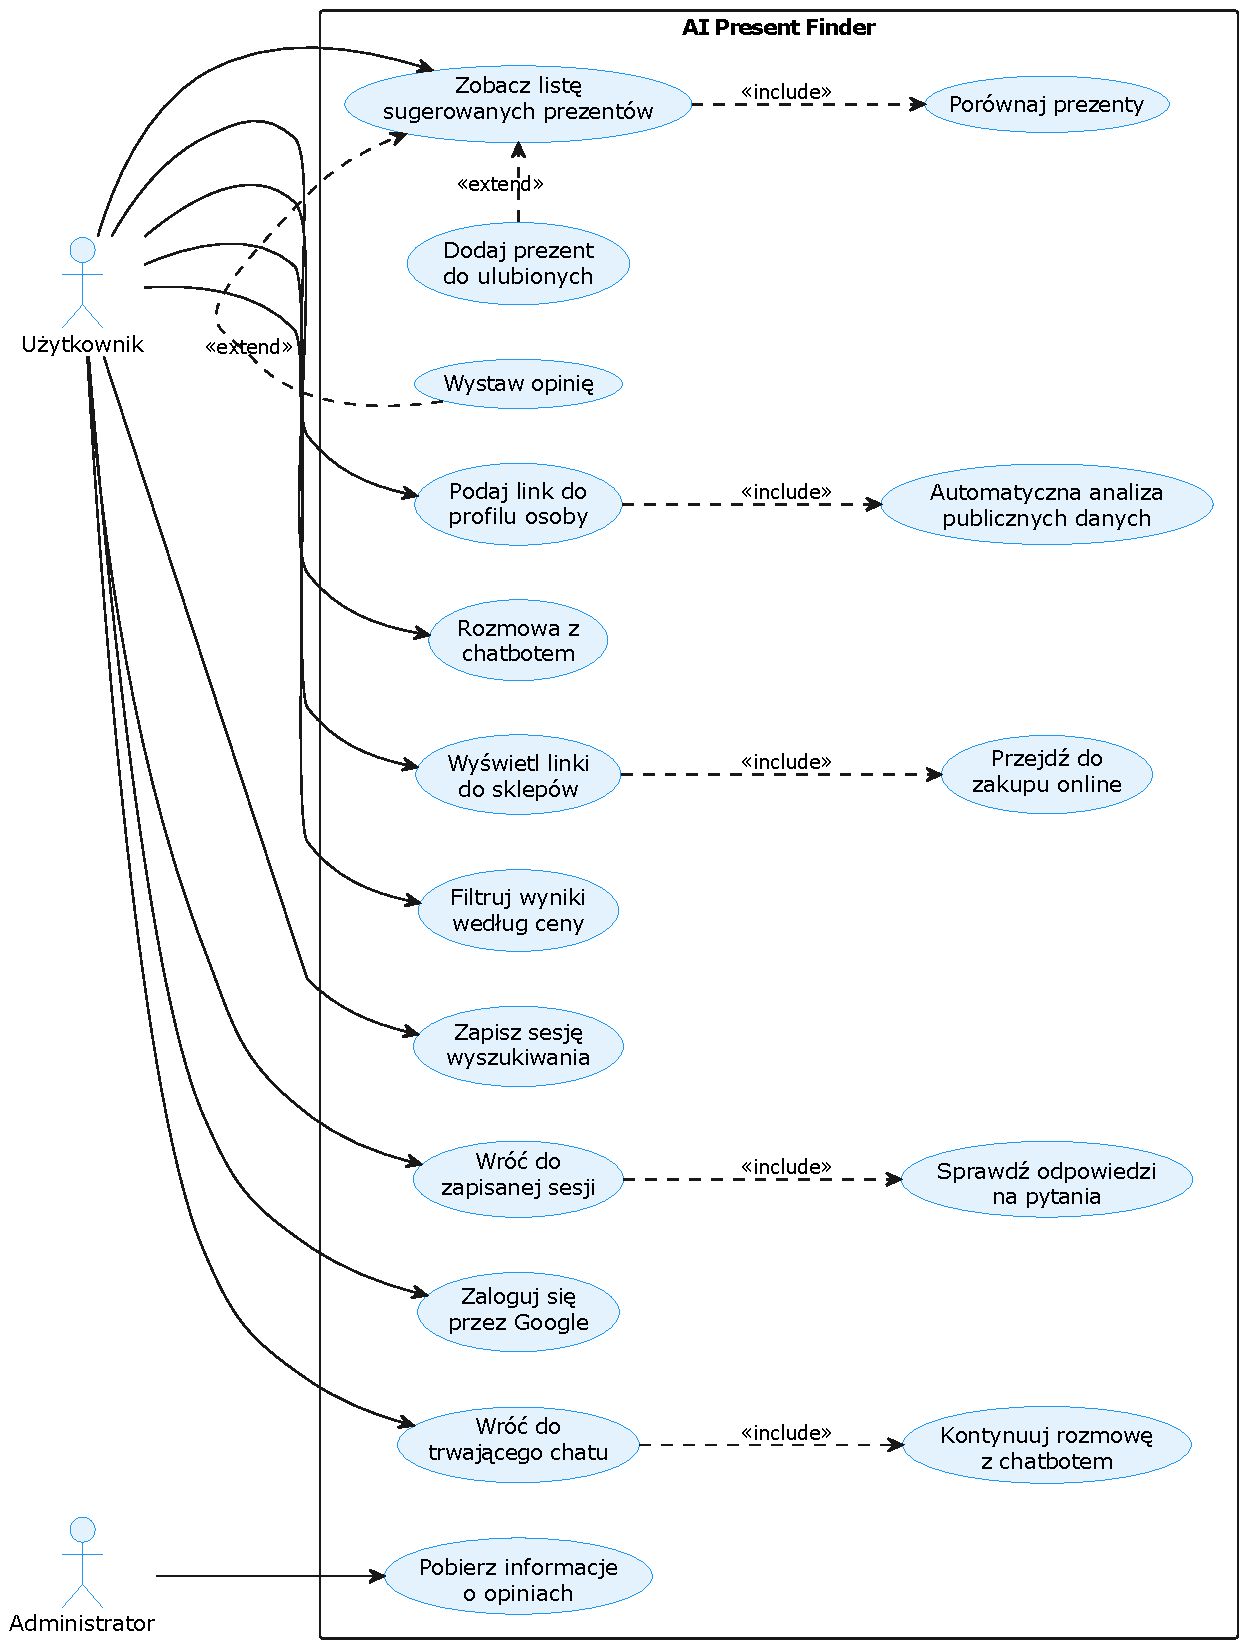
\includegraphics[width=0.85\textwidth]{../use_case_diagram/use_case_diagram.pdf}
    \caption{Diagram przypadków użycia systemu AI Present Finder.}
    \label{fig:use-case}
\end{figure}

\section{Specyfikacja wymagań na produkt programowy}

Poniższa specyfikacja formalizuje wymagania zidentyfikowane w trakcie kolejnych iteracji i pracy z backlogiem, tak aby można je było jednoznacznie odwzorować w architekturze i implementacji.

\subsection{Wymagania funkcjonalne}
\begin{itemize}
    \item \textbf{Wprowadzanie danych:} Możliwość podania linków do profili społecznościowych (Instagram, TikTok).
    \item \textbf{Ekstrakcja danych:} Automatyczne pobranie i analiza publicznych danych z podanych profili.
    \item \textbf{Konwersacja:} Interaktywny chat z botem dopytującym o szczegóły (okazja, budżet, relacja).
    \item \textbf{Analiza:} Łączenie danych z wywiadu i OSINT w spójny profil psychometryczny.
    \item \textbf{Generowanie pomysłów:} Stworzenie listy 5–10 abstrakcyjnych pomysłów na prezent.
    \item \textbf{Wyszukiwanie ofert:} Pobieranie konkretnych ofert z platform e-commerce (OLX, Allegro, Amazon, eBay).
    \item \textbf{Filtrowanie:} Możliwość sortowania i filtrowania wyników (np. po cenie).
\end{itemize}

\subsection{Wymagania niefunkcjonalne}
\begin{itemize}
    \item \textbf{Dostępność:} Aplikacja działa w przeglądarce internetowej bez konieczności instalacji.
    \item \textbf{Wydajność:} Czas generowania wstępnych propozycji nie powinien przekraczać 10 sekund (dla chatu), a pełne wyszukiwanie ofert powinno odbywać się w tle z podglądem postępu.
    \item \textbf{Bezpieczeństwo:} Komunikacja szyfrowana protokołem HTTPS.
    \item \textbf{Skalowalność:} Architektura mikroserwisowa umożliwiająca łatwe dodawanie nowych źródeł danych.
    \item \textbf{Obsługa błędów:} Odporność na limity API zewnętrznych serwisów (mechanizmy ponawiania).
\end{itemize}

\section{Projekt produktu programowego}

Zdefiniowane wymagania funkcjonalne i niefunkcjonalne zostały odwzorowane w poniższej architekturze mikroserwisowej, obejmującej zarówno warstwę frontendową, jak i zestaw współpracujących usług backendowych.

\subsection{Architektura systemu}
System został zaprojektowany w architekturze mikroserwisowej, co zapewnia skalowalność i separację odpowiedzialności. Komunikacja między serwisami odbywa się asynchronicznie za pośrednictwem kolejki wiadomości RabbitMQ.

Główne komponenty systemu:
\begin{itemize}
    \item \textbf{Frontend (React):} Interfejs użytkownika komunikujący się z backendem przez REST API oraz odbierający aktualizacje w czasie rzeczywistym przez SSE (Server-Sent Events).
    \item \textbf{restapi-macroservice (RestAPI Macroservice):} Brama wejściowa (API Gateway), obsługująca żądania HTTP i przekierowująca je do odpowiednich kolejek.
    \item \textbf{chat-microservice (Chat Microservice):} Odpowiada za prowadzenie wywiadu z użytkownikiem.
    \item \textbf{stalking-microservice (Stalking Microservice):} Realizuje proces OSINT (analiza profili społecznościowych).
    \item \textbf{gift-ideas-microservice (Gift Ideas Microservice):} Generuje abstrakcyjne pomysły na prezenty na podstawie zebranych danych.
    \item \textbf{fetch-microservice (Fetch Microservice):} Agreguje oferty z zewnętrznych platform (OLX, Allegro, Amazon, eBay). Działa w wielu instancjach równolegle.
    \item \textbf{reranking-microservice (Reranking Microservice):} Ocenia i filtruje znalezione oferty przy użyciu AI.
\end{itemize}

\subsection{Poziom 1: Kontekst systemu}

Na najwyższym poziomie abstrakcji (C4 Context) system AI Present Finder jest postrzegany jako pojedynczy blok współpracujący z aktorami zewnętrznymi: użytkownikiem szukającym prezentu, platformami e-commerce (OLX, Allegro, Amazon, eBay), mediami społecznościowymi (Instagram, TikTok) oraz dostawcami modeli LLM (OpenAI, Google). Zależności te przedstawiono na Rysunku~\ref{fig:c4-context}.

\begin{figure}[ht]
    \centering
    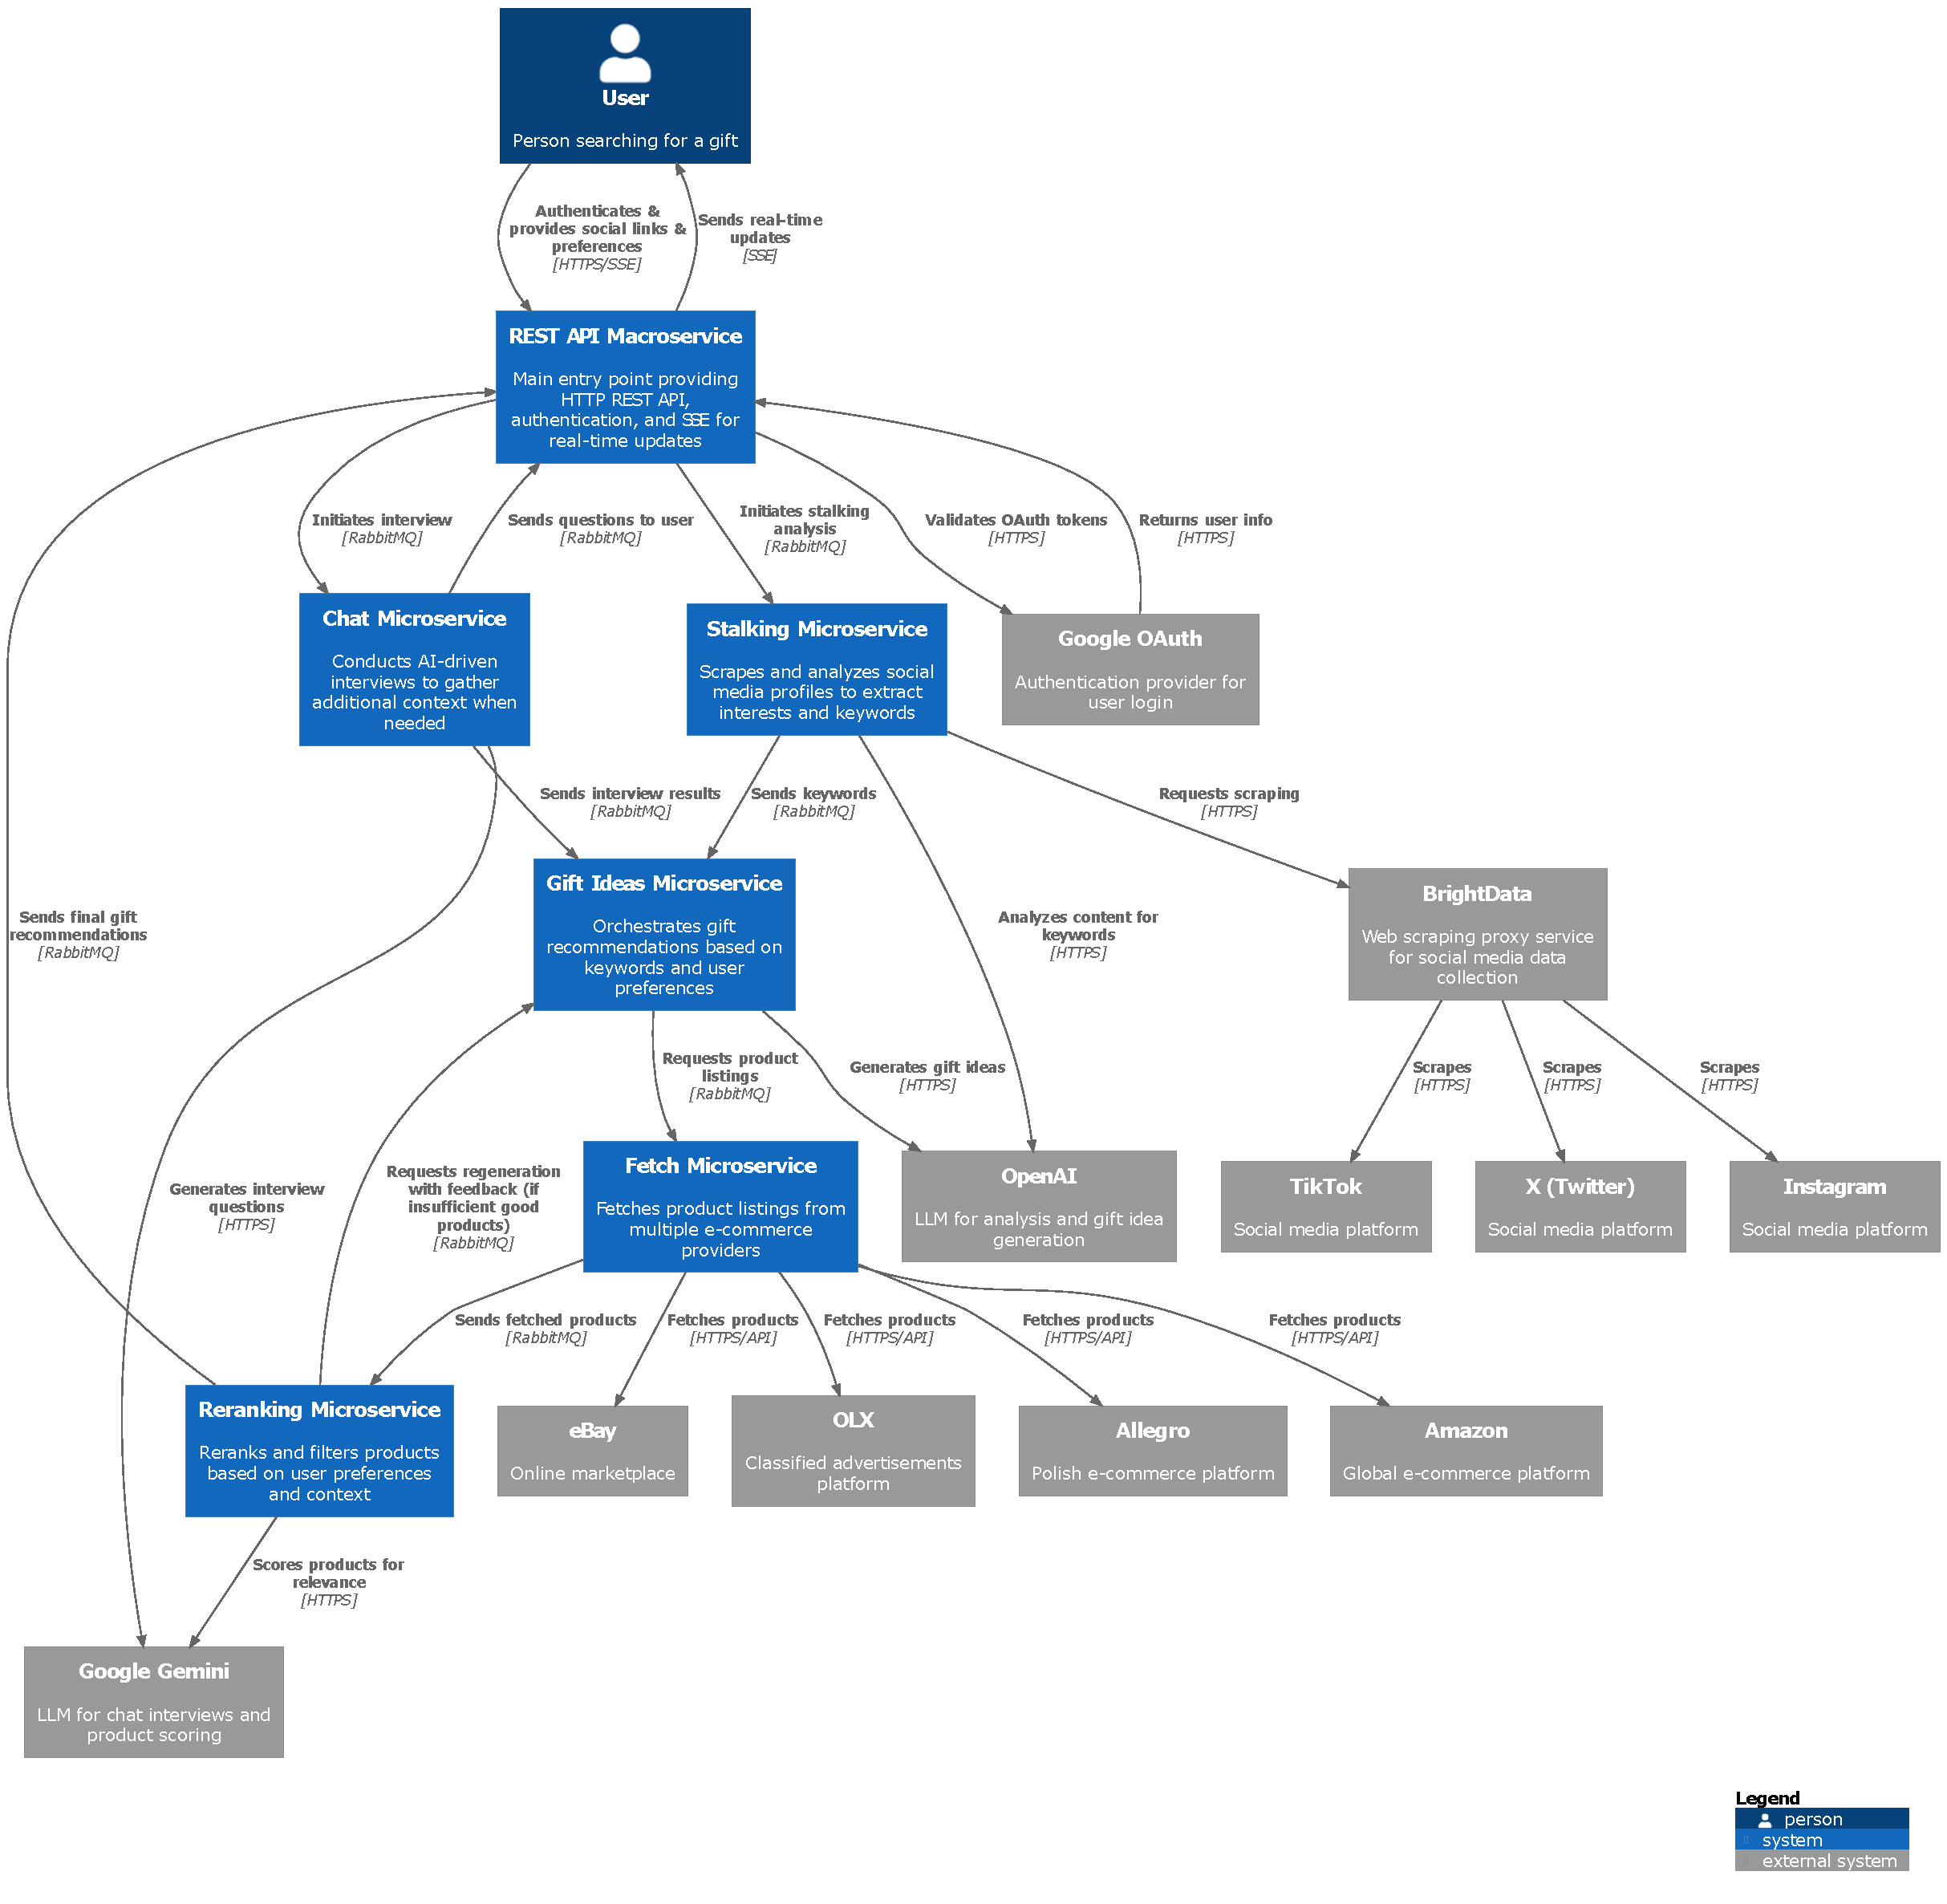
\includegraphics[width=0.85\textwidth]{../C4_v0.2.0/C4_Context_MVP.pdf}
    \caption{Diagram kontekstowy systemu AI Present Finder (C4 Context).}
    \label{fig:c4-context}
\end{figure}

\subsection{Poziom 2: Kontenery}

Po zejściu o jeden poziom niżej (C4 Container) widać podział systemu na odrębne jednostki wdrożeniowe: aplikację frontendową (React SPA), bramę API (restapi-macroservice), zestaw mikroserwisów backendowych, bazę danych PostgreSQL oraz broker wiadomości RabbitMQ. Każdy kontener może być niezależnie skalowany i wdrażany w środowisku Docker/Coolify. Architekturę kontenerów przedstawiono na Rysunku~\ref{fig:c4-container}.

\clearpage
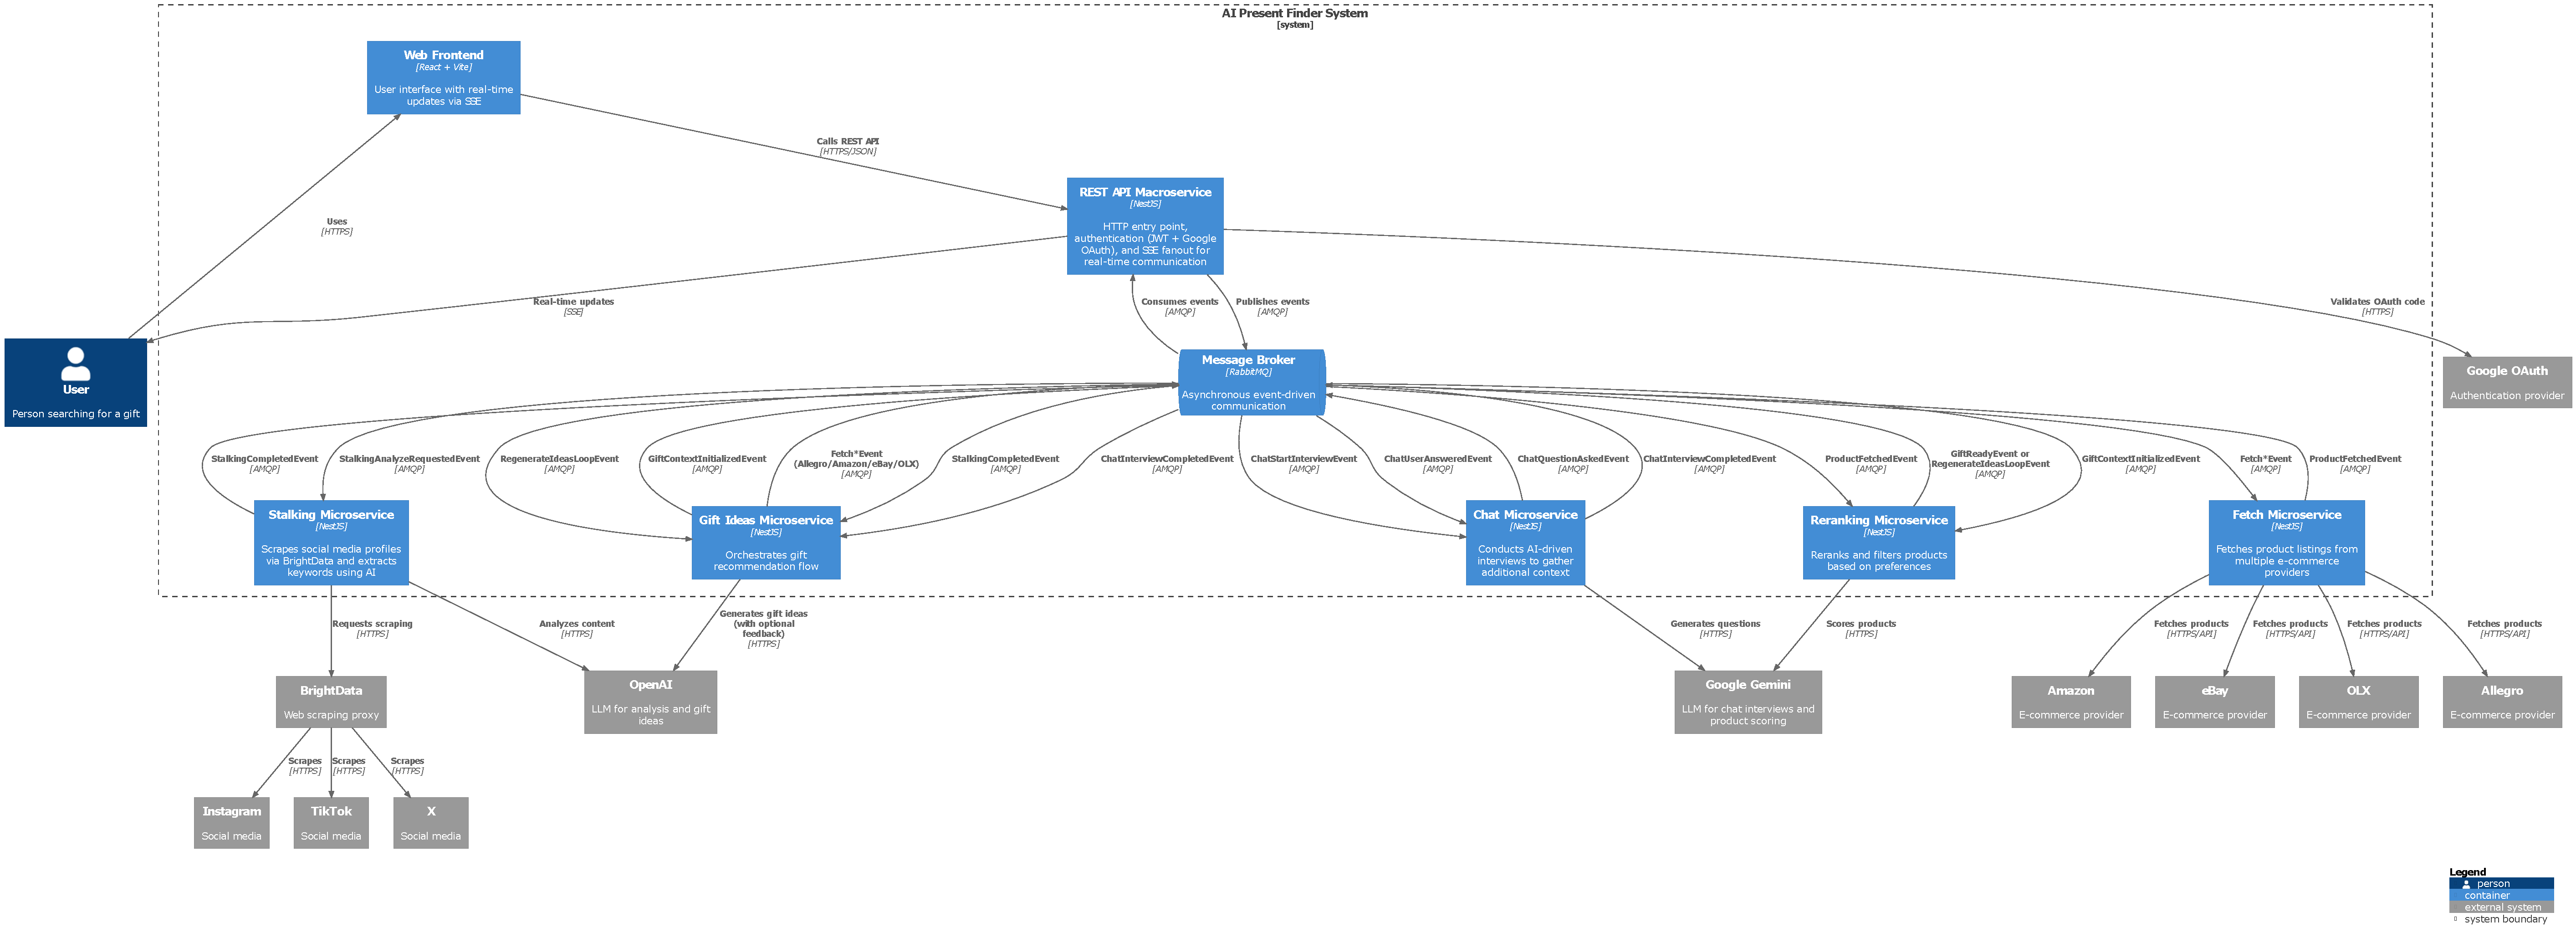
\includepdf[pages=1,landscape=true,pagecommand={\thispagestyle{plain}\refstepcounter{figure}\addcontentsline{lof}{figure}{\protect\numberline{\thefigure}Diagram kontenerów systemu AI Present Finder (C4 Container)}},fitpaper=true]{../C4_v0.2.0/C4_Container.pdf}
\label{fig:c4-container}
\addtocounter{figure}{-1}
\refstepcounter{figure}
\clearpage

\subsection{Poziom 3: Komponenty wybranych mikroserwisów}

Na najniższym prezentowanym poziomie (C4 Component) każdy mikroserwis jest rozbity na wewnętrzne moduły. Poniżej przedstawiono trzy kluczowe serwisy.

\paragraph{RestAPI Macroservice.}
Brama wejściowa systemu (Rysunek~\ref{fig:c4-component-restapi}) składa się z warstwy kontrolerów HTTP, handlerów komend CQRS oraz adapterów publikujących zdarzenia do kolejek RabbitMQ. Odpowiada również za obsługę SSE i autoryzację (Google OAuth).

\clearpage

\includepdf[pages=1,landscape=true,pagecommand={\thispagestyle{plain}\refstepcounter{figure}\addcontentsline{lof}{figure}{\protect\numberline{\thefigure}Diagram komponentów RestAPI Macroservice (C4 Component)}},fitpaper=true]{../C4_v0.2.0/C4_Component_RestAPI.pdf}
\label{fig:c4-component-restapi}
\addtocounter{figure}{-1}
\refstepcounter{figure}
\clearpage

\paragraph{Chat Microservice.}
Serwis prowadzący wywiad z użytkownikiem (Rysunek~\ref{fig:c4-component-chat}) wykorzystuje mechanizm \textit{tool calling}, aby wymusić strukturyzowane odpowiedzi od modelu LLM. Wewnętrznie dzieli się na handler zdarzeń, flow AI oraz repozytorium sesji.

\begin{figure}[ht]
    \centering
    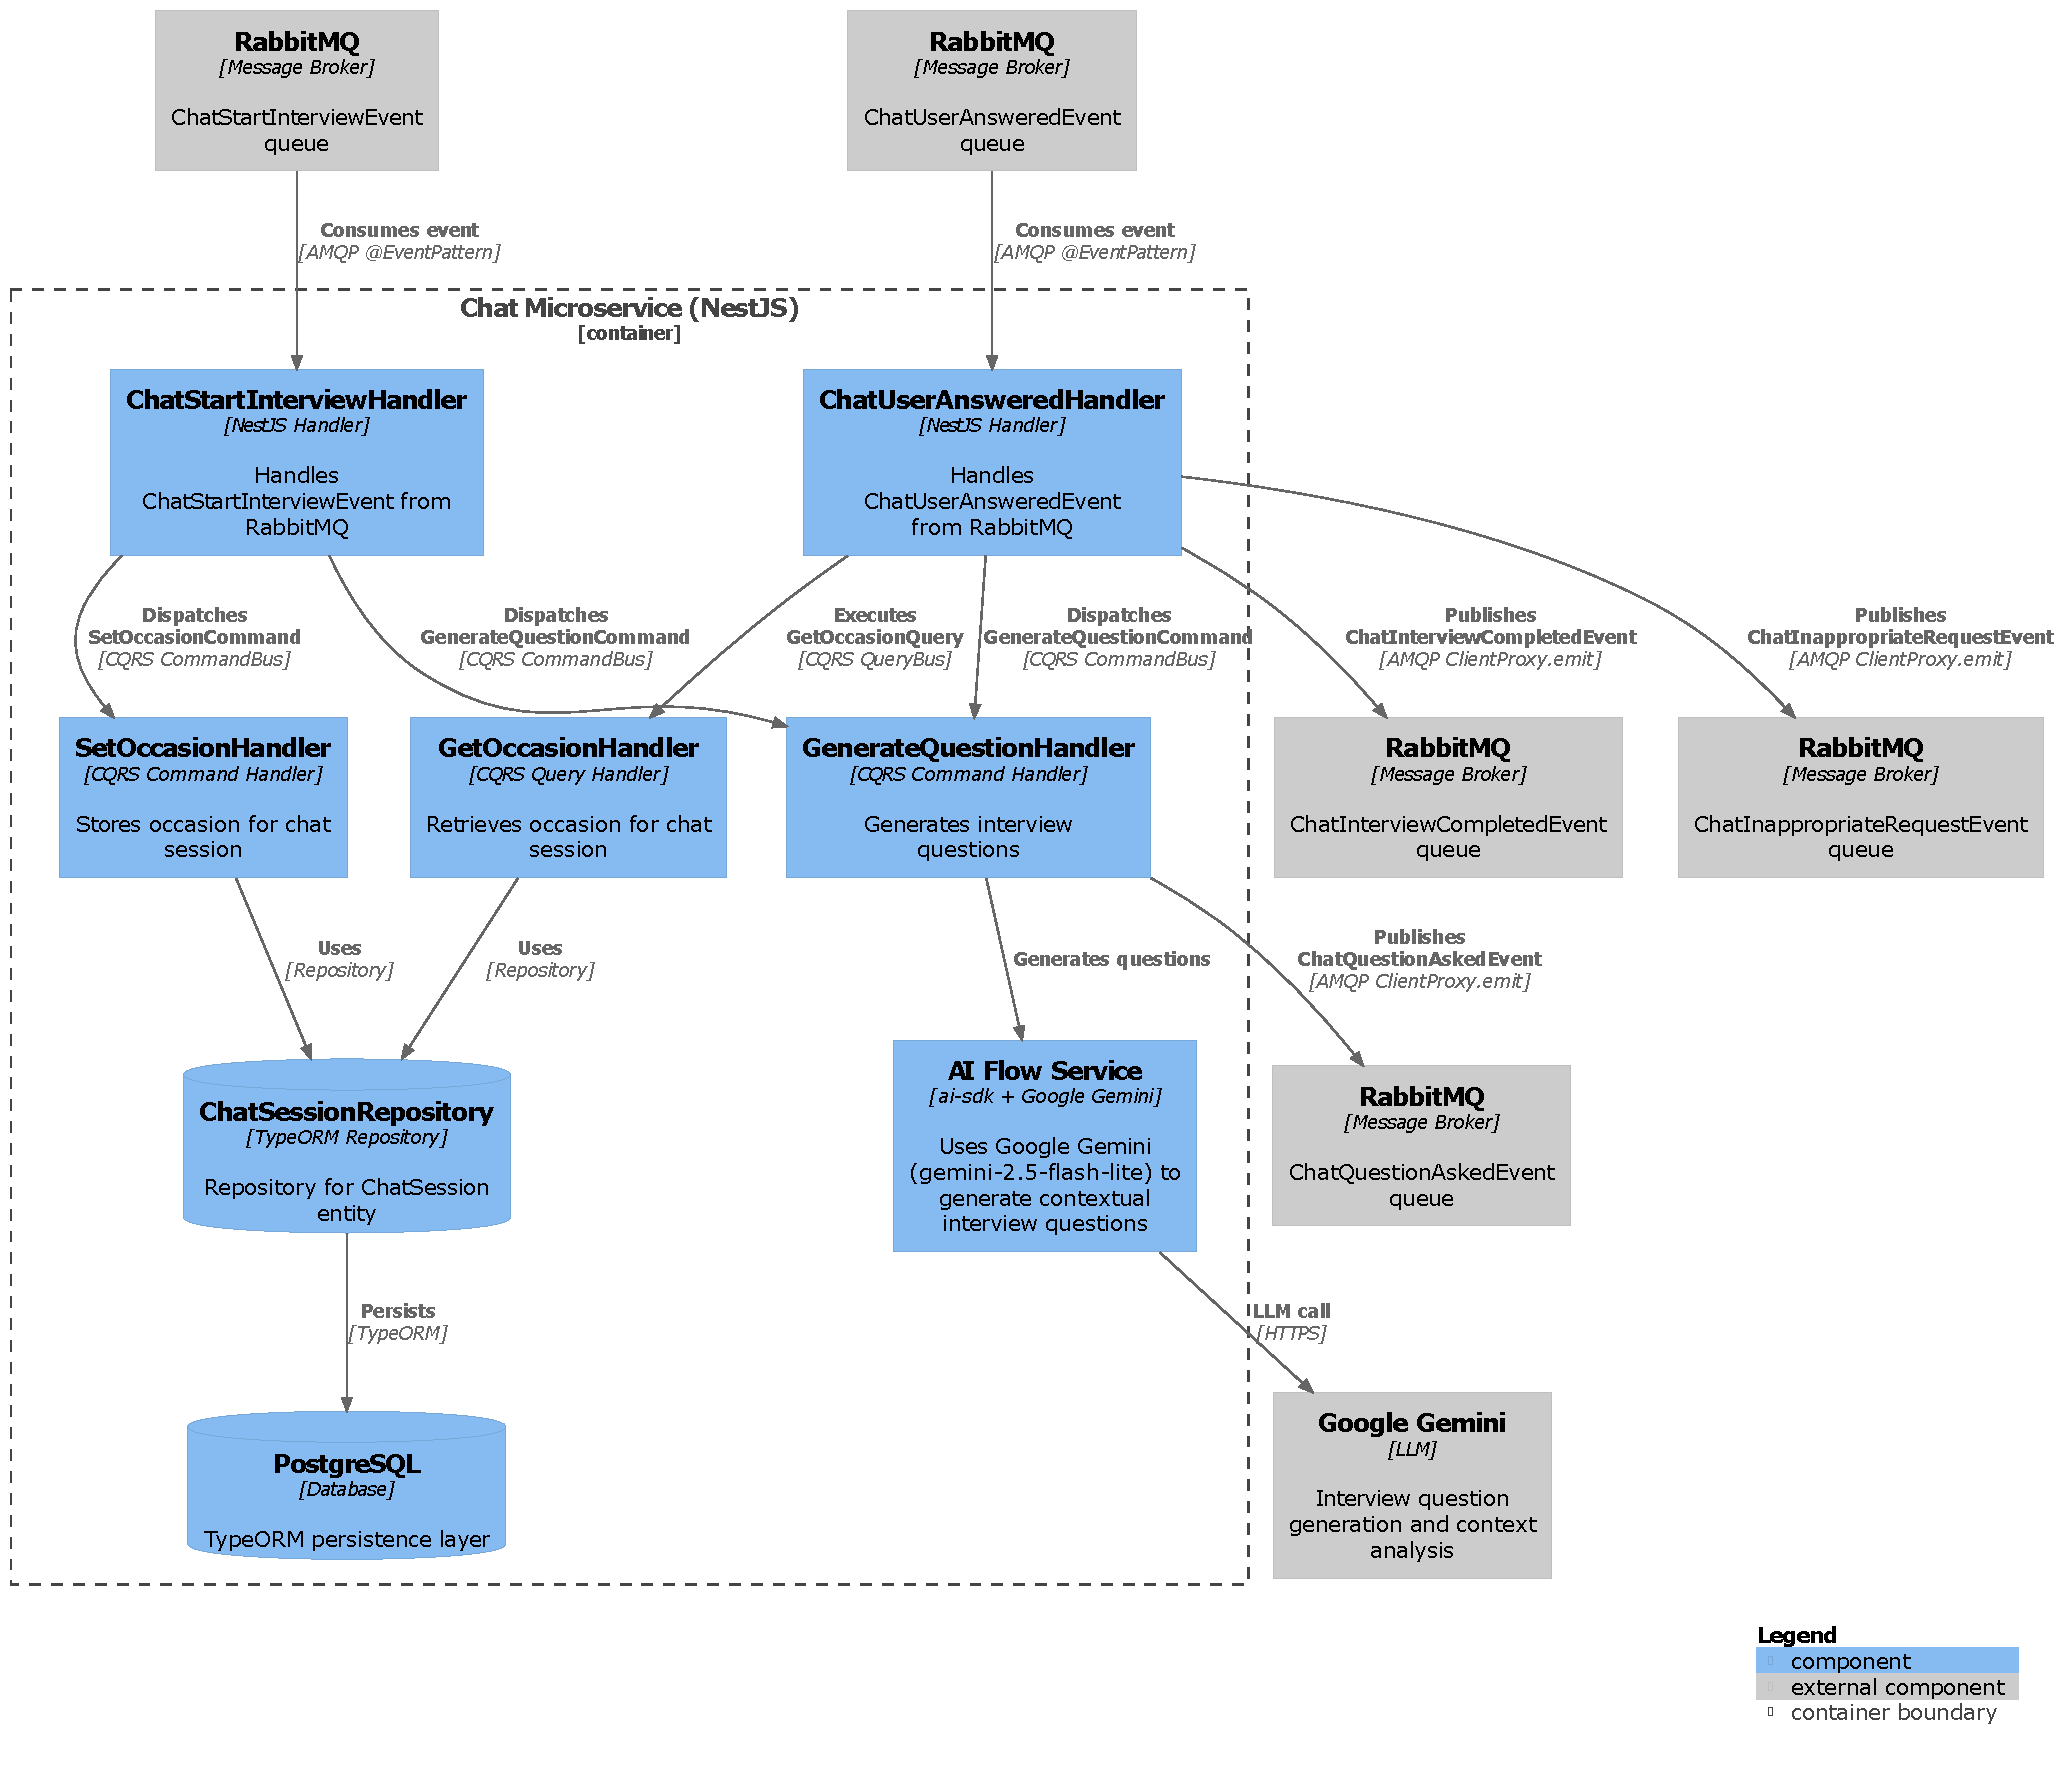
\includegraphics[width=0.82\textwidth]{../C4_v0.2.0/C4_Component_Chat.pdf}
    \caption{Diagram komponentów Chat Microservice (C4 Component).}
    \label{fig:c4-component-chat}
\end{figure}

\paragraph{Reranking Microservice.}
Moduł odpowiedzialny za ocenę i filtrowanie ofert (Rysunek~\ref{fig:c4-component-reranking}) korzysta z modelu Gemini 2.5 do semantycznej analizy każdego produktu. Generuje ocenę punktową oraz tekstowe uzasadnienie, co zapewnia wyjaśnialność decyzji (XAI).

\clearpage
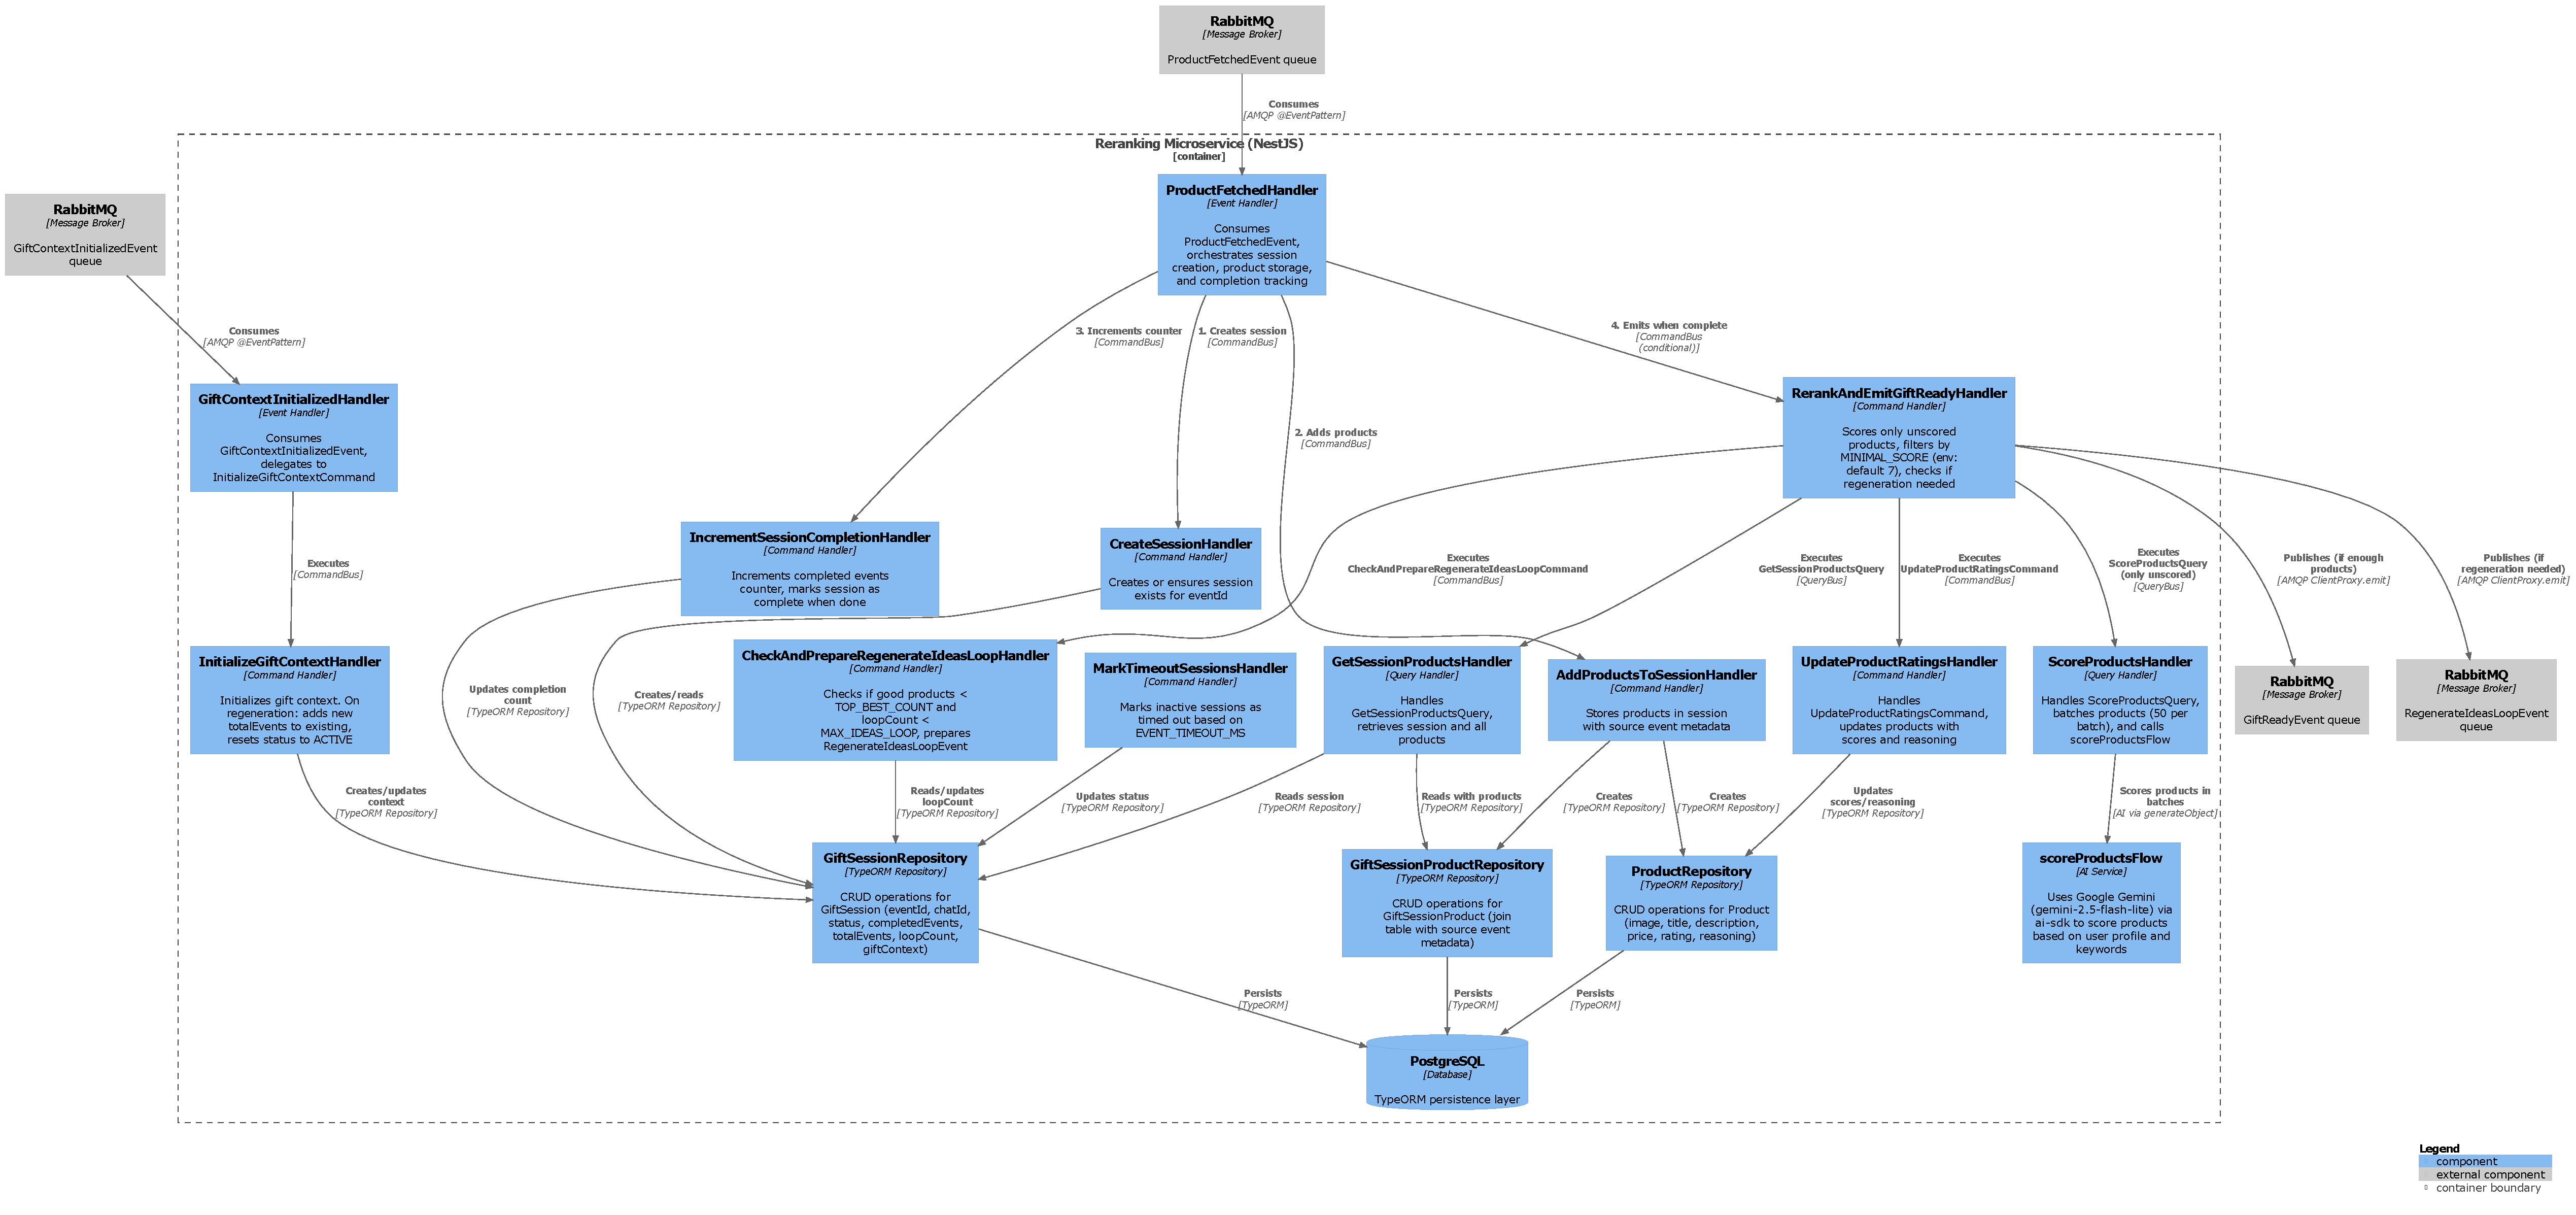
\includepdf[pages=1,landscape=true,pagecommand={\thispagestyle{plain}\refstepcounter{figure}\addcontentsline{lof}{figure}{\protect\numberline{\thefigure}Diagram komponentów Reranking Microservice (C4 Component)}},fitpaper=true]{../C4_v0.2.0/C4_Component_Reranking.pdf}
\label{fig:c4-component-reranking}
\addtocounter{figure}{-1}
\refstepcounter{figure}
\clearpage

\subsection{Zastosowane wzorce projektowe}
\begin{itemize}
    \item \textbf{CQRS (Command Query Responsibility Segregation):} Rozdzielenie operacji modyfikujących stan (Command) od zapytań o dane (Query).
    \item \textbf{Event-Driven Architecture:} System reaguje na zdarzenia (np. \texttt{StalkingCompletedEvent}, \texttt{ProductFetchedEvent}), co pozwala na luźne powiązanie komponentów.
    \item \textbf{Asynchronous Request-Reply:} Obsługa długotrwałych procesów bez blokowania wątku głównego.
    \item \textbf{Strategy:} Wybór odpowiedniego algorytmu pobierania danych w zależności od źródła (np. strategia dla OLX vs strategia dla Amazon).
    \item \textbf{DTO (Data Transfer Object):} Ustrukturyzowane obiekty do przesyłania danych między warstwami.
\end{itemize}

\subsection{Powiązanie z modelami C4}
Architektura systemu została zaprojektowana zgodnie z podejściem C4 i odwzorowana na trzech pierwszych poziomach:
\begin{itemize}
    \item \textbf{Poziom 1 – Context:} AI Present Finder jako system wspierający proces wyboru prezentu, współpracujący z użytkownikiem, promotorem (w roli interesariusza) oraz zewnętrznymi dostawcami (sklepy, media społecznościowe, dostawcy LLM).
    \item \textbf{Poziom 2 – Container:} Podział systemu na frontend (przeglądarka), backend (RestAPI, mikroserwisy), bazę danych oraz RabbitMQ. Każdy z mikroserwisów jest osobnym kontenerem uruchamianym w środowisku Docker/Coolify.
    \item \textbf{Poziom 3 – Component:} W ramach każdego mikroserwisu wyróżniono komponenty takie jak kontrolery HTTP, handlery zdarzeń, serwisy domenowe oraz warstwę dostępu do danych (repozytoria TypeORM).
\end{itemize}
Diagramy C4 (context, container, component) zostały przygotowane w narzędziu PlantUML i są spójne z opisem wymagań oraz podziałem na mikroserwisy przedstawionym w tej sekcji.

\section{Model danych i baza danych}

Aby wesprzeć zdefiniowane przypadki użycia i przyjętą architekturę mikroserwisową, zaprojektowano model danych odzwierciedlający kluczowe byty domenowe oraz ich relacje.

\subsection{Model konceptualny}
Model danych został zaprojektowany w sposób domenowy, z wykorzystaniem diagramów E/R oraz UML (diagram klas). Główne byty to m.in.:
\begin{itemize}
    \item \textbf{User} – reprezentuje zalogowanego użytkownika systemu (dane z Google OAuth, preferencje),
    \item \textbf{Session} – pojedyncza sesja wyszukiwania prezentów, powiązana z użytkownikiem,
    \item \textbf{ChatMessage} – wiadomości w ramach sesji (pytania i odpowiedzi),
    \item \textbf{GiftIdea} – abstrakcyjny pomysł na prezent wygenerowany przez moduł AI,
    \item \textbf{Product} – konkretna oferta produktu pobrana z serwisu e-commerce,
    \item \textbf{Feedback} – ocena użytkownika dotycząca trafności rekomendacji,
    \item \textbf{Favorite} – relacja użytkownika do wybranych produktów (lista ulubionych).
\end{itemize}
Relacje między tymi bytami zostały odwzorowane na diagramie konceptualnym (User posiada wiele Session; Session posiada wiele ChatMessage i GiftIdea; GiftIdea powiązana jest z wieloma Product; User może dodawać Product do Favorites oraz pozostawiać Feedback dla Session). Na Rysunku~\ref{fig:class-diagram} przedstawiono diagram klas UML modelu domenowego, natomiast fizyczną strukturę tabel w bazie PostgreSQL pokazuje diagram E/R na Rysunku~\ref{fig:er-diagram}.

\clearpage
\begin{figure}[p]
    \centering
    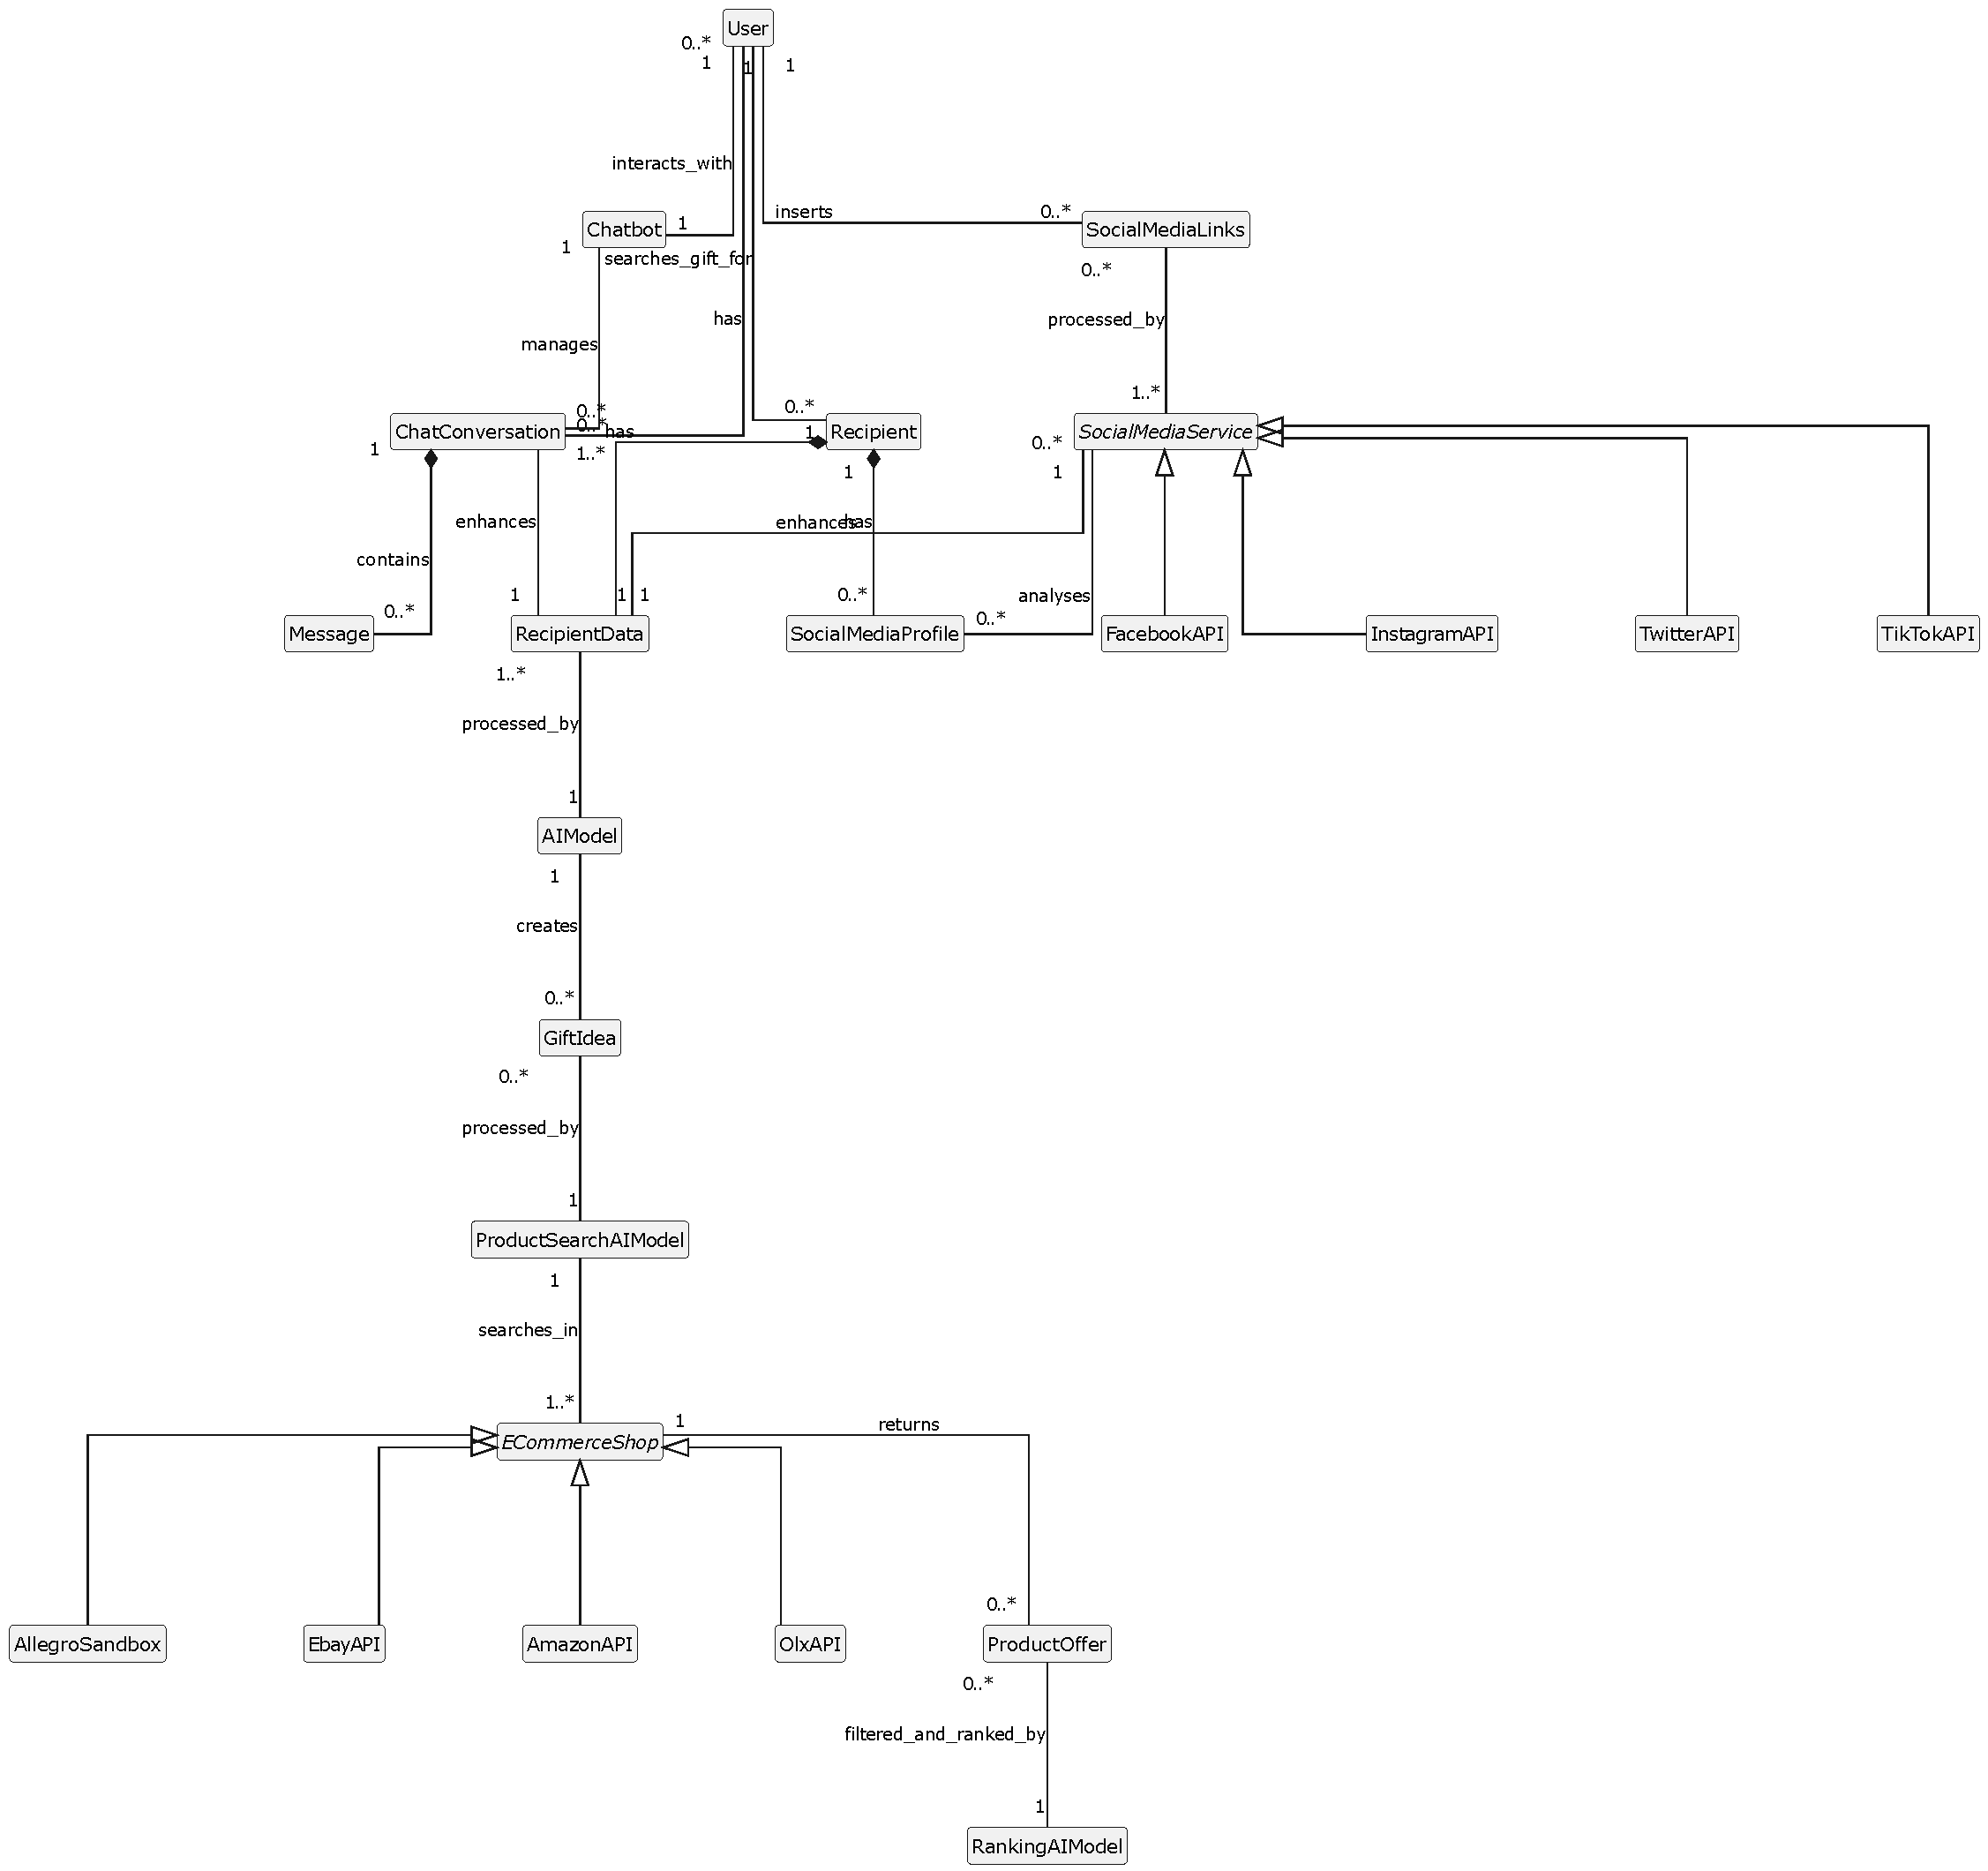
\includegraphics[width=\textwidth,height=0.9\textheight,keepaspectratio]{../class_diagram/domain_class_diagram.pdf}
    \caption{Diagram klas UML modelu domenowego systemu.}
    \label{fig:class-diagram}
\end{figure}
\clearpage

\begin{figure}[ht]
    \centering
    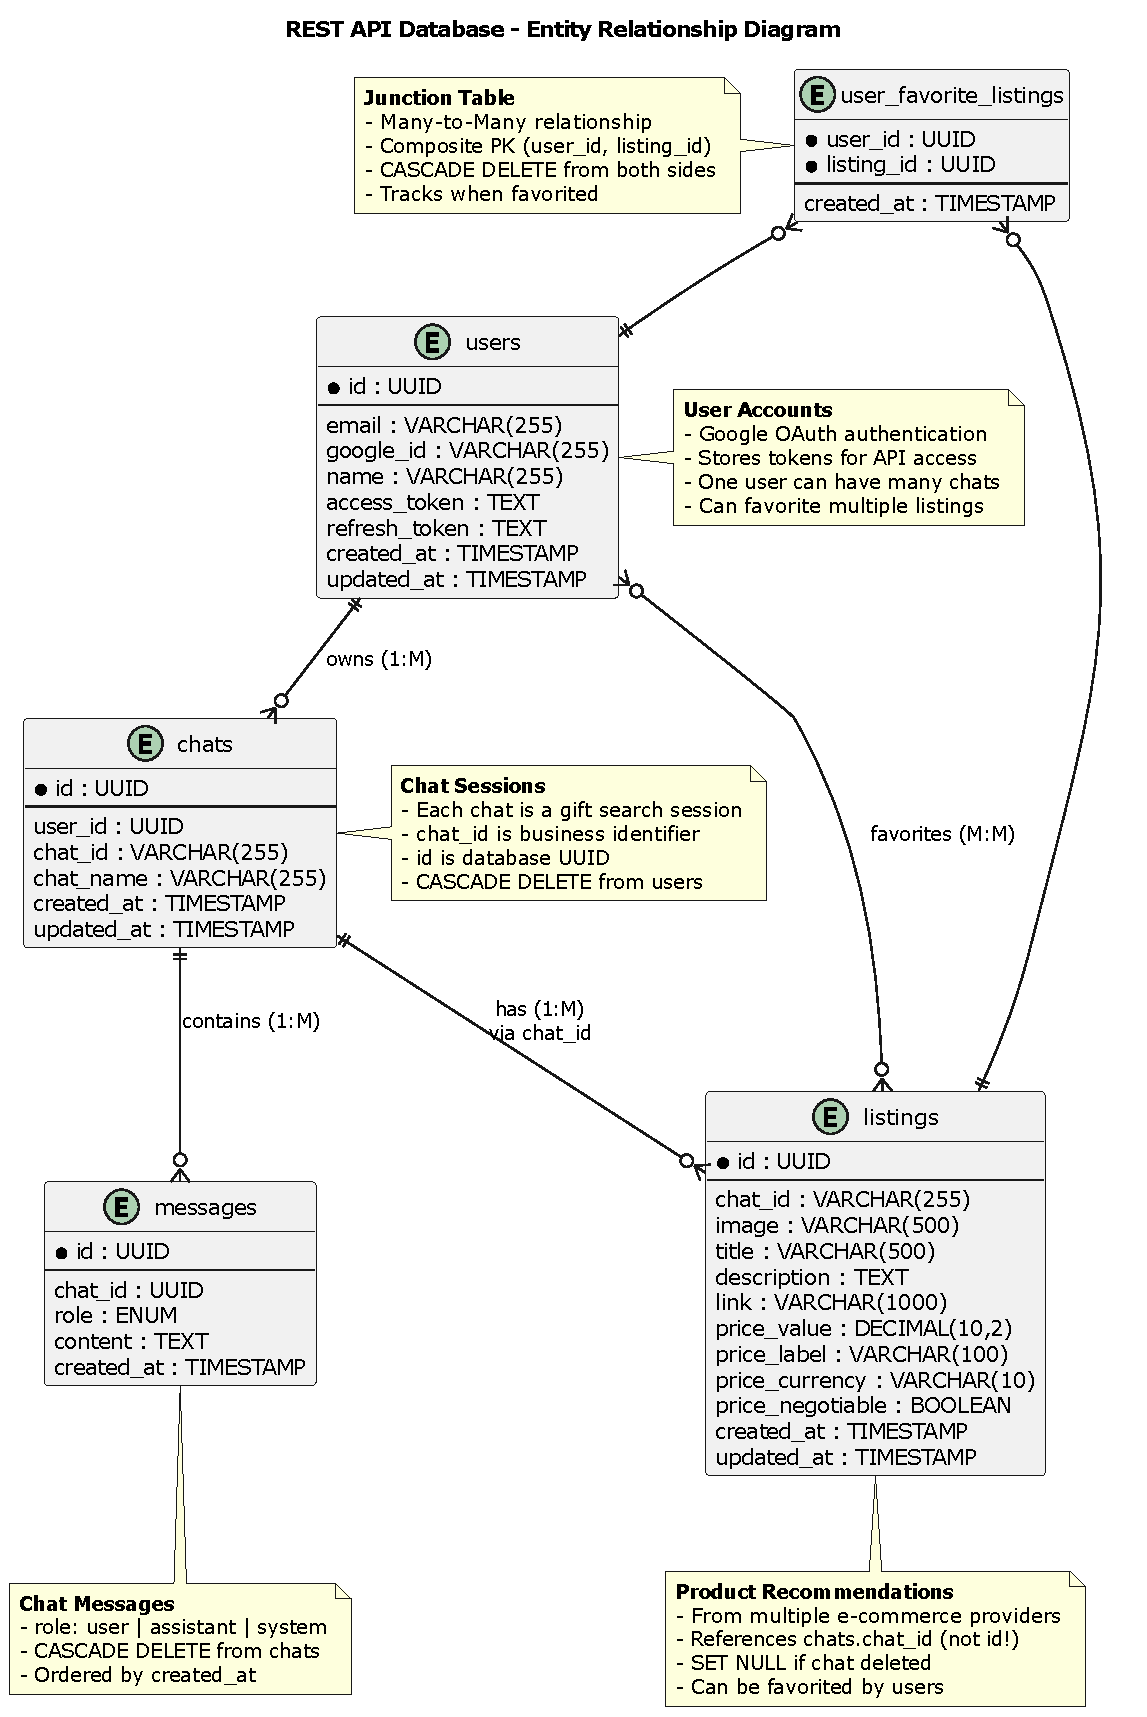
\includegraphics[width=0.9\textwidth]{../databases/restapi/restapi_er_diagram.pdf}
    \caption{Diagram E/R modelu danych głównej bazy (RestAPI).}
    \label{fig:er-diagram}
\end{figure}

\subsection{Implementacja w DBMS}
Implementację modelu danych wykonano w PostgreSQL z wykorzystaniem TypeORM. Dla każdej encji domenowej przygotowano odpowiadającą jej tabelę, z kluczami głównymi typu UUID oraz indeksami przyspieszającymi wyszukiwanie po polach takich jak \texttt{userId}, \texttt{sessionId} czy \texttt{provider} (OLX, Allegro, eBay, Amazon).

Początkowo używano trybu \texttt{synchronize: true}, jednak na etapie wdrożenia produkcyjnego przełączono się na migracje bazodanowe, aby zapewnić kontrolę nad zmianami schematu. Migracje generowano narzędziem CLI TypeORM i uruchamiano w pipeline CI/CD oraz na serwerze produkcyjnym.

W dokumentacji bazy danych wyróżniono widok całościowy (diagram wszystkich tabel) oraz zbliżenia na kluczowe fragmenty, takie jak model sesji i historii wyszukiwań czy model przechowywania feedbacku użytkowników.

\section{Modelowanie behawioralne}

Po ustaleniu struktury systemu kluczowe było opisanie jego zachowania w czasie w postaci sekwencji interakcji, stanów oraz procesów biznesowych, które prowadzą użytkownika od podania linku aż do listy konkretnych ofert prezentów.

\subsection{Diagram sekwencji}
Dla głównego scenariusza użycia (wyszukiwanie prezentu) przygotowano diagram sekwencji UML (Rysunek~\ref{fig:sequence-main}) przedstawiający przepływ wiadomości pomiędzy: Użytkownikiem, Frontendem, RestAPI Macroservice, Chat Microservice, Stalking Microservice, Gift Ideas Microservice, Fetch Microservice oraz Reranking Microservice. Diagram pokazuje m.in. moment, w którym Chat Microservice decyduje o rozpoczęciu wyszukiwania oraz sposób, w jaki wyniki są strumieniowane do użytkownika przez SSE.

\clearpage
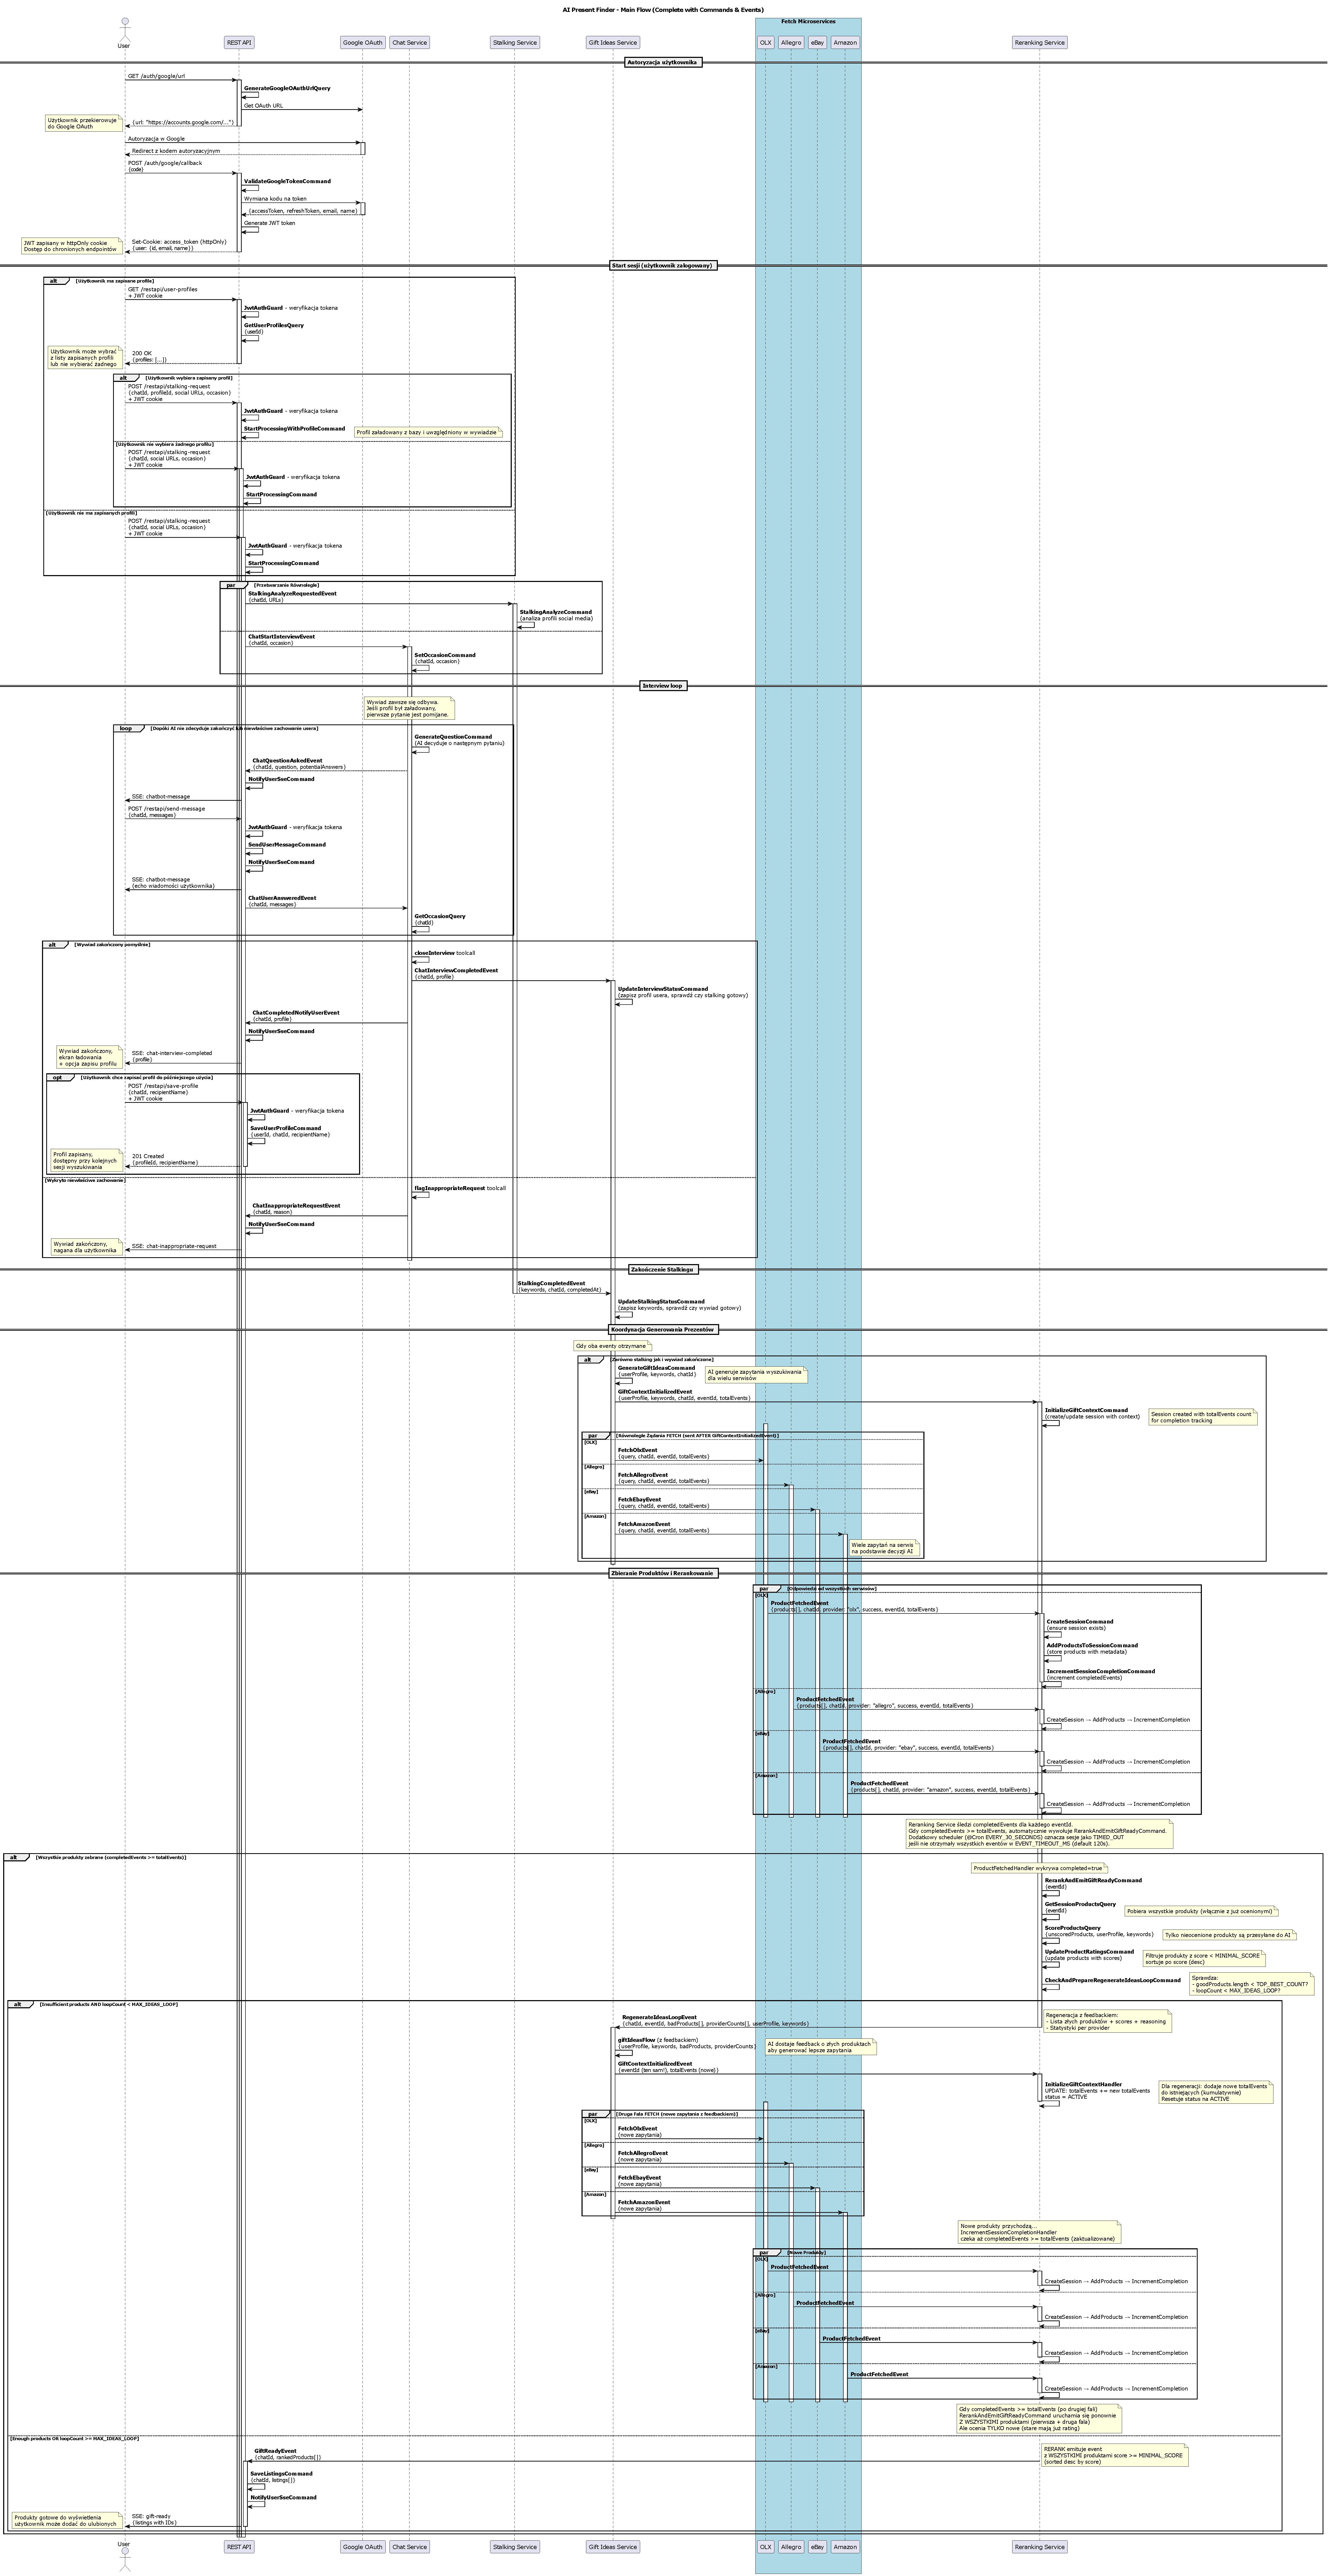
\includepdf[pages=1,landscape=true,pagecommand={\thispagestyle{plain}\refstepcounter{figure}\addcontentsline{lof}{figure}{\protect\numberline{\thefigure}Diagram sekwencji głównego przepływu wyszukiwania prezentu}},fitpaper=true]{../sequence_diagram/main_flow/main_flow.pdf}
\label{fig:sequence-main}
\addtocounter{figure}{-1}
\refstepcounter{figure}
\clearpage

\subsection{Diagramy stanów i aktywności}
Stan aplikacji z perspektywy sesji użytkownika został opisany za pomocą diagramu stanów (stany: \textit{Nowa}, \textit{Wywiad}, \textit{Wyszukiwanie}, \textit{Prezentacja wyników}, \textit{Refinement}, \textit{Zakończona}). Dla wybranych operacji (np. flow rerankingu oraz przetwarzania profilu społecznościowego) przygotowano także diagramy aktywności, które obrazują równoległe gałęzie przetwarzania (scraping wielu sklepów jednocześnie).

\subsection{BPMN}
Proces biznesowy od momentu wejścia użytkownika na stronę (landing page) do zakończenia sesji wyszukiwania został odwzorowany w notacji BPMN (Rysunek~\ref{fig:bpmn}). Diagram przedstawia m.in. decyzje użytkownika (kontynuować wywiad vs. przejść od razu do wyników), punkty integracji z zewnętrznymi API oraz miejsca potencjalnych błędów (np. brak odpowiedzi od dostawcy), wraz z obsługą wyjątków.

\clearpage
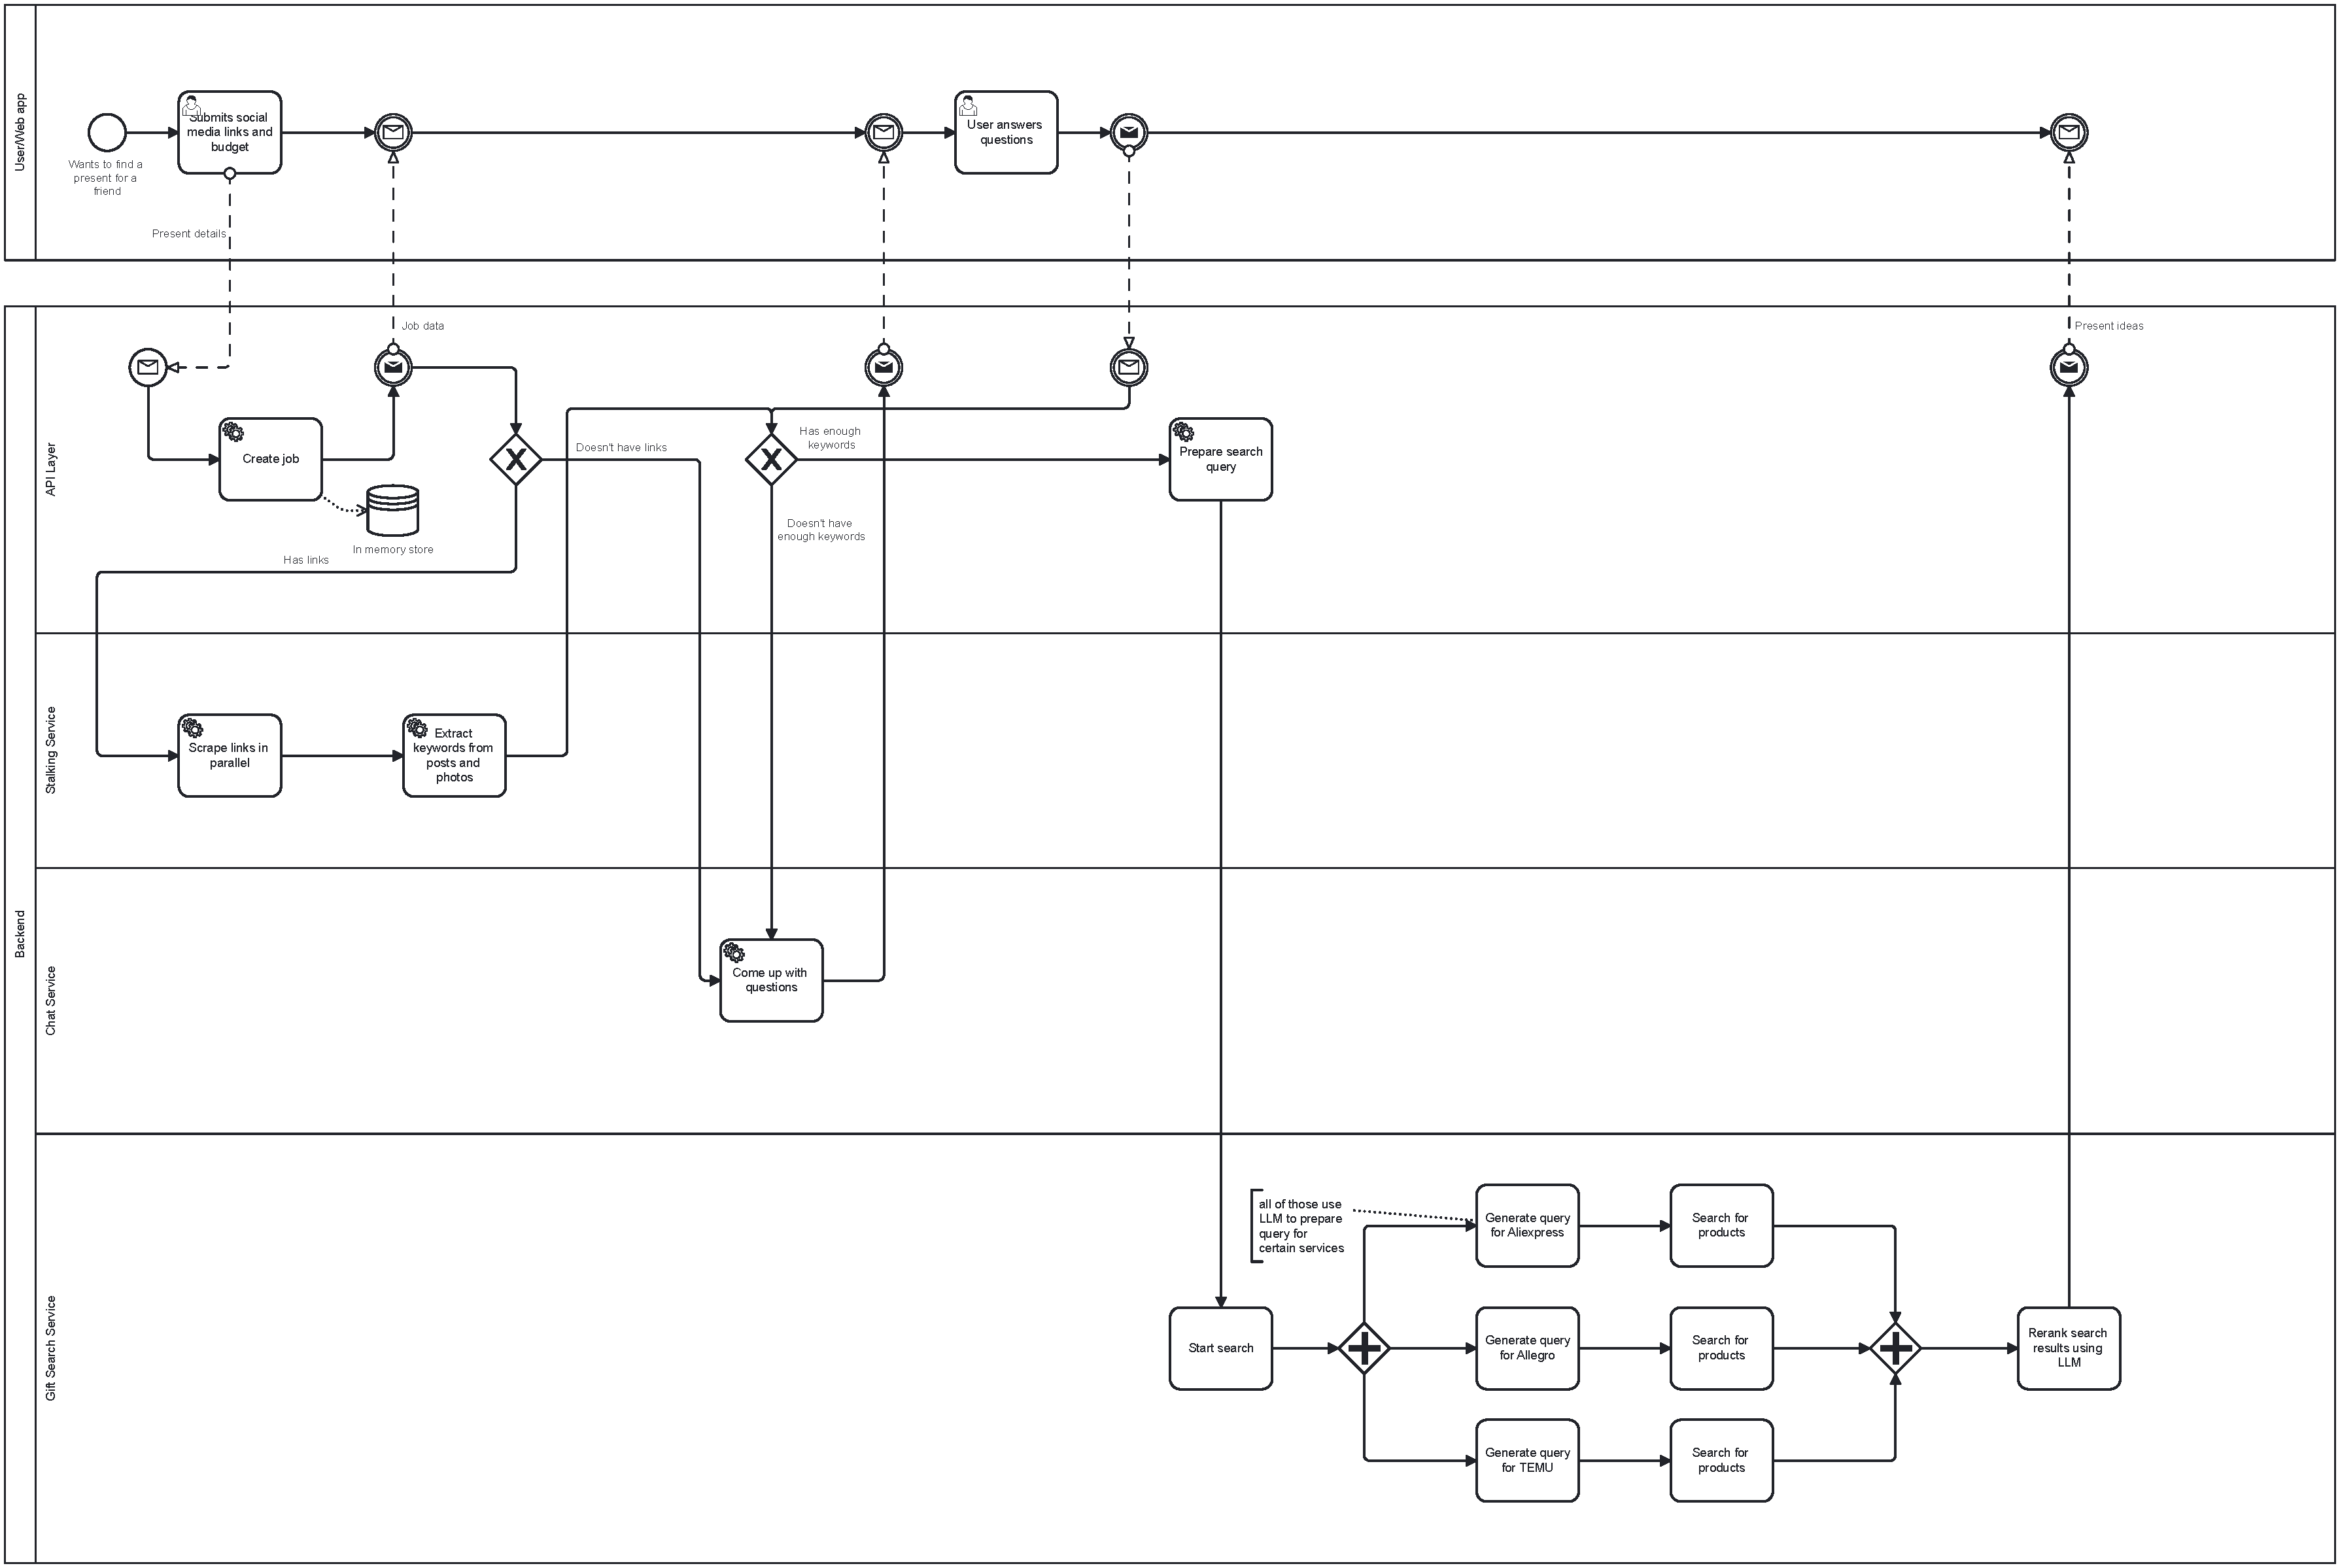
\includepdf[pages=1,landscape=true,pagecommand={\thispagestyle{plain}\refstepcounter{figure}\addcontentsline{lof}{figure}{\protect\numberline{\thefigure}Diagram BPMN procesu wyszukiwania prezentu w systemie}},fitpaper=true]{../BPMN/diagram.pdf}
\label{fig:bpmn}
\addtocounter{figure}{-1}
\refstepcounter{figure}
\clearpage

\section{Prototypowanie interfejsu}

Na podstawie powyższych modeli zaprojektowano interfejs użytkownika, który prowadzi odbiorcę przez najważniejsze przepływy w możliwie naturalny i zrozumiały sposób.

Interfejs użytkownika powstawał iteracyjnie, w ścisłym powiązaniu z modelem wymagań i architektury. W narzędziu Figma przygotowano prototypy widoków, które następnie przekładano na komponenty React (Shadcn UI + Tailwind), zachowując spójność z przepływami zdefiniowanymi na diagramach C4, UML i BPMN.

Poniżej przedstawiono pełne flow użytkownika – od wejścia na stronę, przez konfigurację wyszukiwania i wywiad z chatbotem, aż do otrzymania spersonalizowanych rekomendacji oraz zarządzania zapisanymi produktami.

\subsection{Krok 1: Strona główna (Landing Page)}

Użytkownik trafia na stronę główną (Rysunek~\ref{fig:ui-landing}), która w prosty sposób przedstawia wartość aplikacji: \textit{,,Znajdź idealny prezent w kilka minut''}. Strona składa się z kilku sekcji:
\begin{itemize}
    \item \textbf{Hero} – główny baner z logo i przyciskiem CTA ,,Rozpocznij'',
    \item \textbf{Jak to działa} – 4 karty opisujące proces (linki społecznościowe → rozmowa z AI → wyszukiwanie → filtrowanie),
    \item \textbf{Zespół} – informacje o twórcach aplikacji,
    \item \textbf{FAQ} – odpowiedzi na najczęściej zadawane pytania.
\end{itemize}

Na tym etapie użytkownik może zalogować się przez Google OAuth, co umożliwia zapisywanie historii sesji i ulubionych produktów.

\subsection{Krok 2: Formularz wyszukiwania}

Po kliknięciu przycisku ,,Rozpocznij'' użytkownik przechodzi do formularza konfiguracji wyszukiwania (Rysunek~\ref{fig:ui-search-form}). Formularz składa się z trzech sekcji:

\textbf{a) Linki do mediów społecznościowych} (opcjonalne) – użytkownik może podać adresy profili Instagram, X (Twitter) lub TikTok obdarowywanej osoby. System wykorzysta publiczne dane do lepszego zrozumienia zainteresowań odbiorcy.

\textbf{b) Wybór okazji} – siatka 4 przycisków pozwala określić kontekst prezentu: Urodziny, Rocznica, Święta, Tak po prostu.

\textbf{c) Budżet} – użytkownik wybiera przedział cenowy (do 50 zł, 50–100 zł, 100–200 zł) lub podaje własny zakres.

\begin{figure}[H]
    \centering
    \begin{subfigure}[t]{0.48\textwidth}
        \centering
        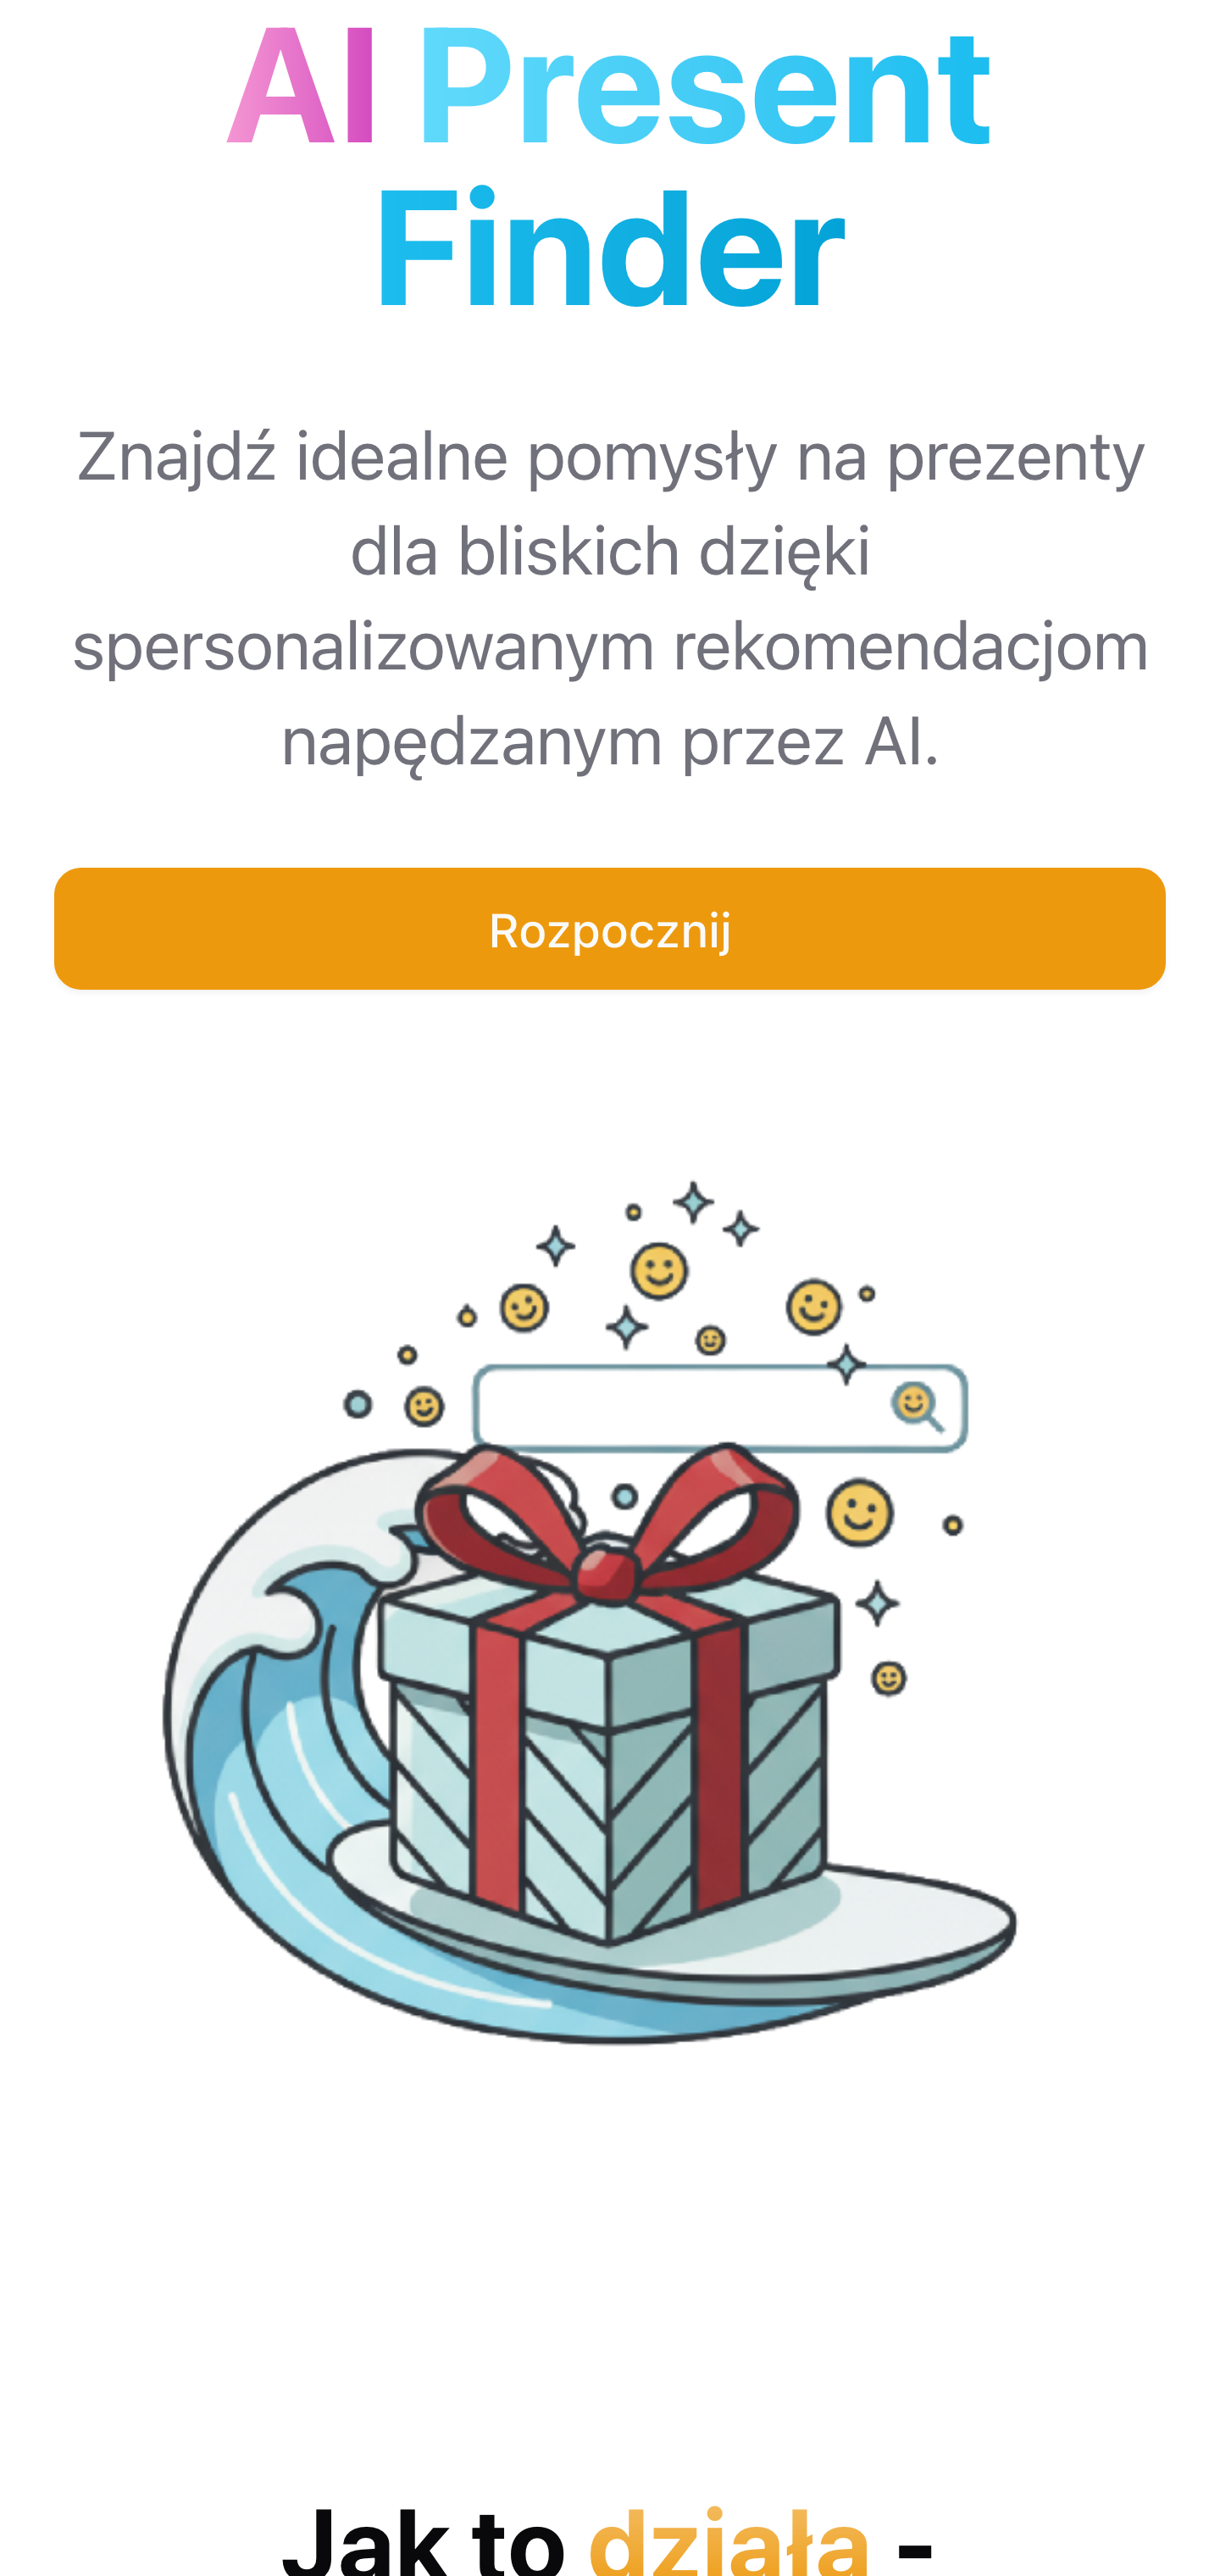
\includegraphics[width=\textwidth]{../designs/landing_page.png}
        \caption{Strona główna (landing page).}
        \label{fig:ui-landing}
    \end{subfigure}
    \hfill
    \begin{subfigure}[t]{0.48\textwidth}
        \centering
        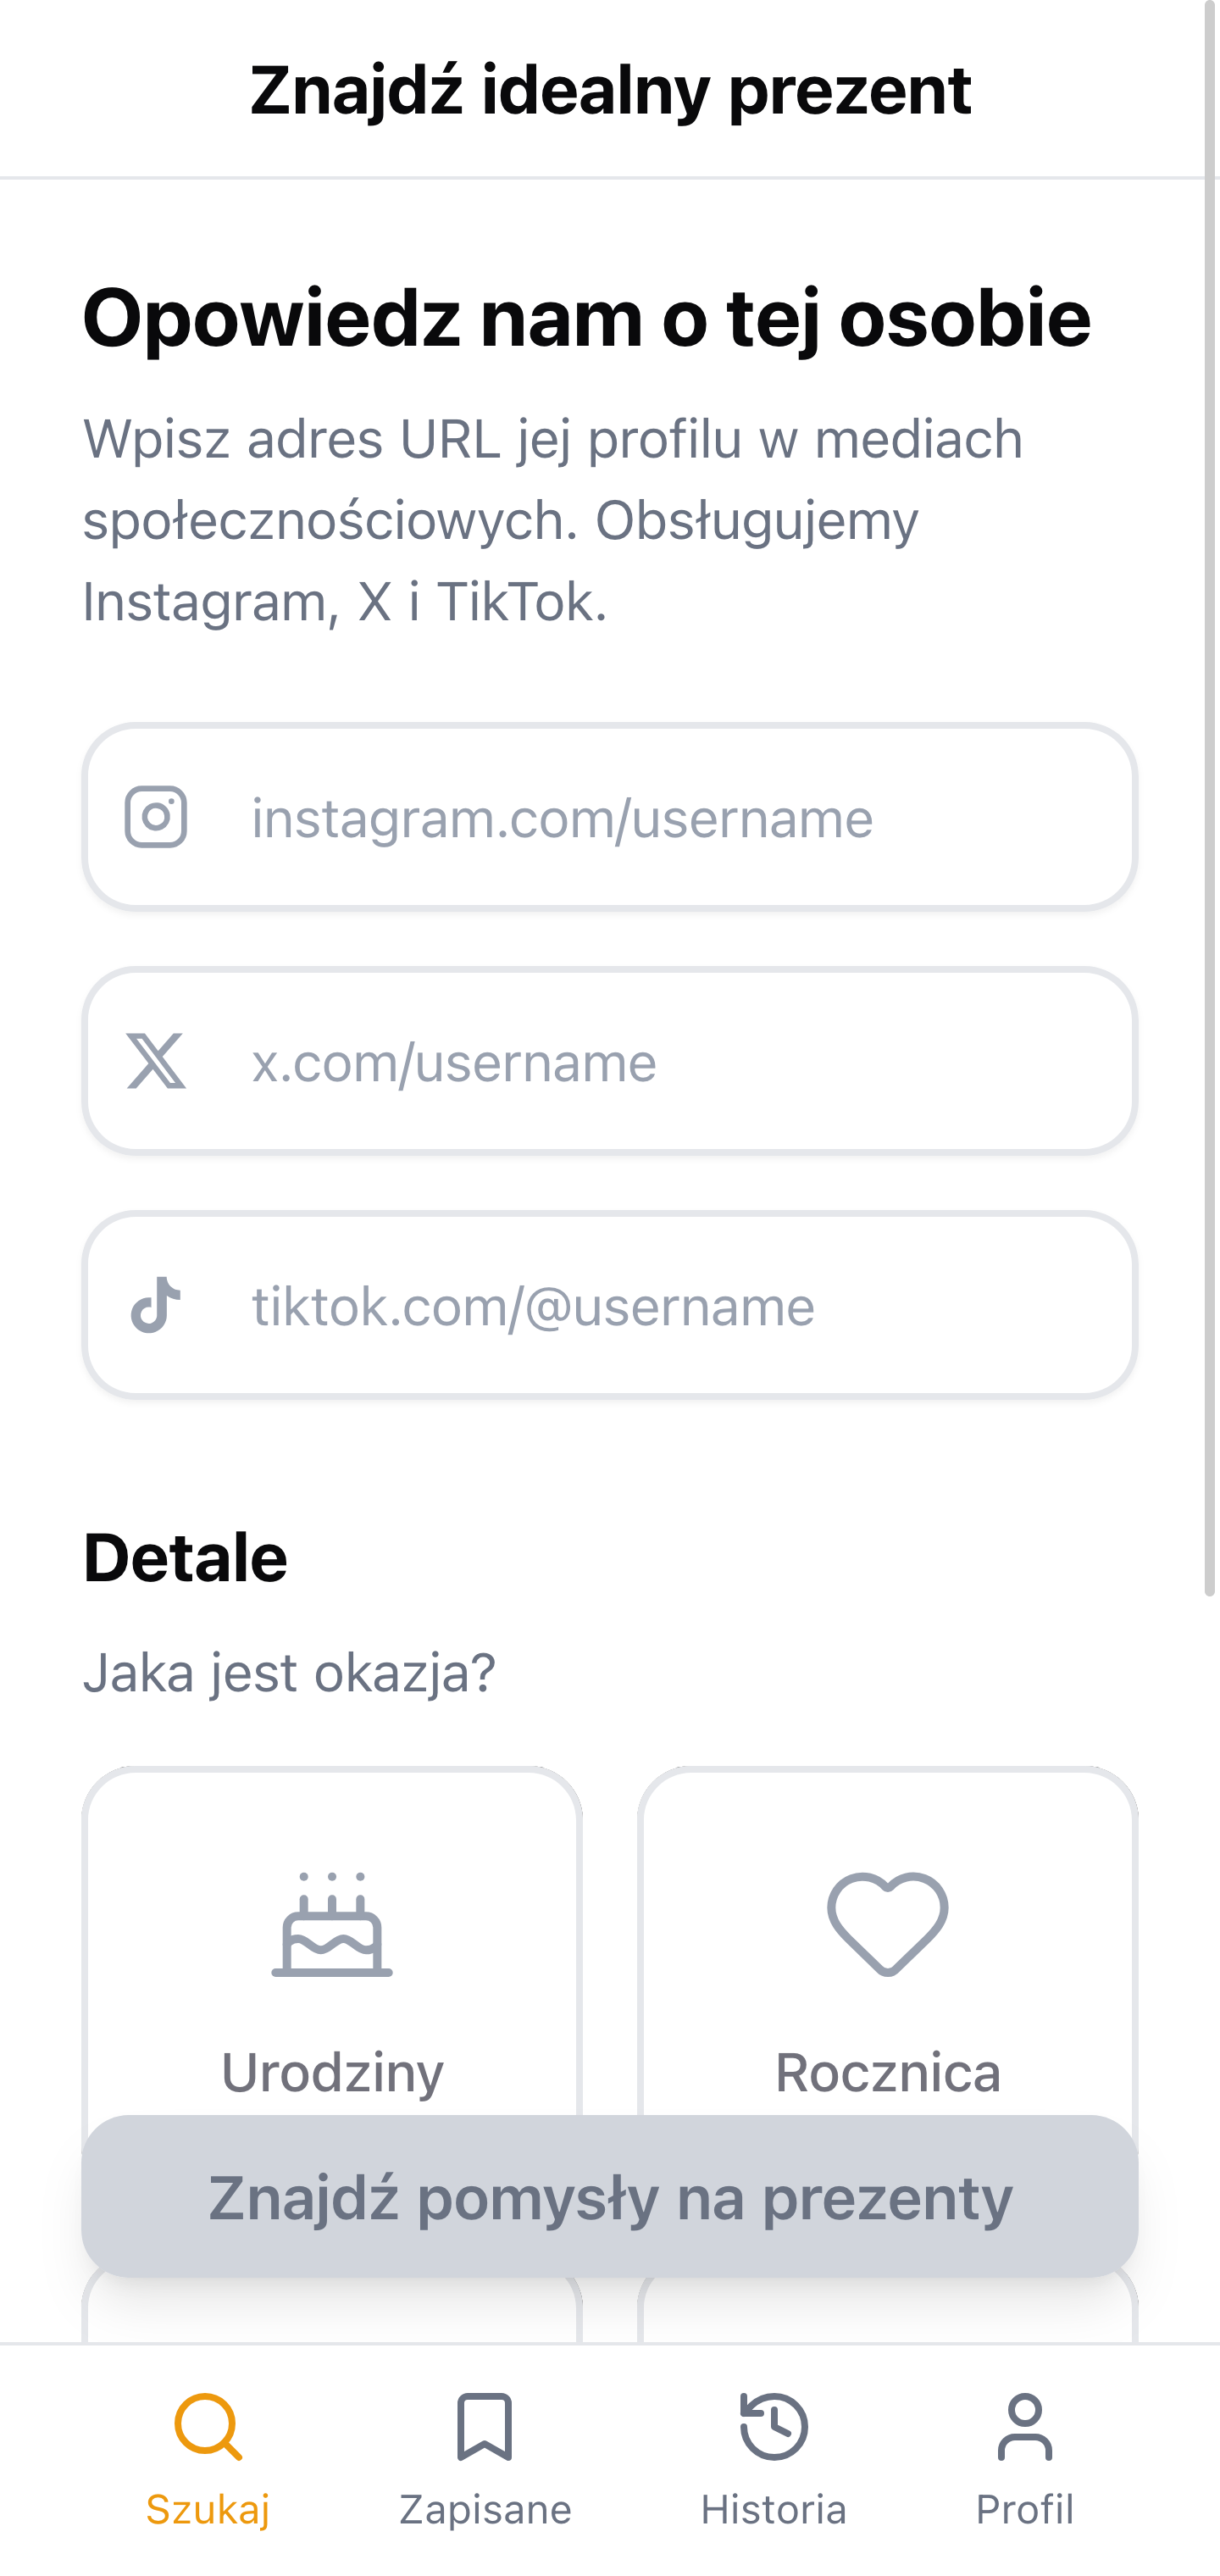
\includegraphics[width=\textwidth]{../designs/start-search.png}
        \caption{Formularz wyszukiwania.}
        \label{fig:ui-search-form}
    \end{subfigure}
    \caption{Początek flow użytkownika: strona główna i formularz konfiguracji wyszukiwania.}
    \label{fig:ui-start-flow}
\end{figure}

Jeśli użytkownik wcześniej szukał prezentu dla tej samej osoby, system zaproponuje wczytanie zapisanego profilu, co przyspiesza proces konfiguracji.

\subsection{Krok 3: Wywiad z chatbotem}

Po wysłaniu formularza użytkownik przechodzi do interfejsu chatu (Rysunek~\ref{fig:ui-chat}). Agent AI prowadzi krótki wywiad, dopytując o szczegóły dotyczące relacji z obdarowywaną osobą, zainteresowań i hobby odbiorcy oraz preferencji stylistycznych.

Chatbot oferuje sugerowane odpowiedzi (przyciski), ale użytkownik może też wpisać własną odpowiedź. Pasek postępu w nagłówku informuje o etapie wywiadu. Cała rozmowa trwa średnio 2–3 minuty i składa się z ok. 8–12 pytań.

\subsection{Krok 4: Lista rekomendacji}

Po zakończeniu wywiadu system analizuje zebrane dane, generuje abstrakcyjne pomysły na prezenty, a następnie wyszukuje konkretne oferty w czterech serwisach e-commerce (OLX, Allegro, Amazon, eBay).

Wyniki są prezentowane w formie przejrzystej siatki kart (Rysunek~\ref{fig:ui-results}), gdzie każda oferta zawiera zdjęcie produktu, badge z nazwą platformy, tytuł, cenę oraz przycisk ,,Kup teraz''. Górna belka oferuje rozbudowane opcje filtrowania oraz tryby doprecyzowania i oceniania.

\begin{figure}[H]
    \centering
    \begin{subfigure}[t]{0.48\textwidth}
        \centering
        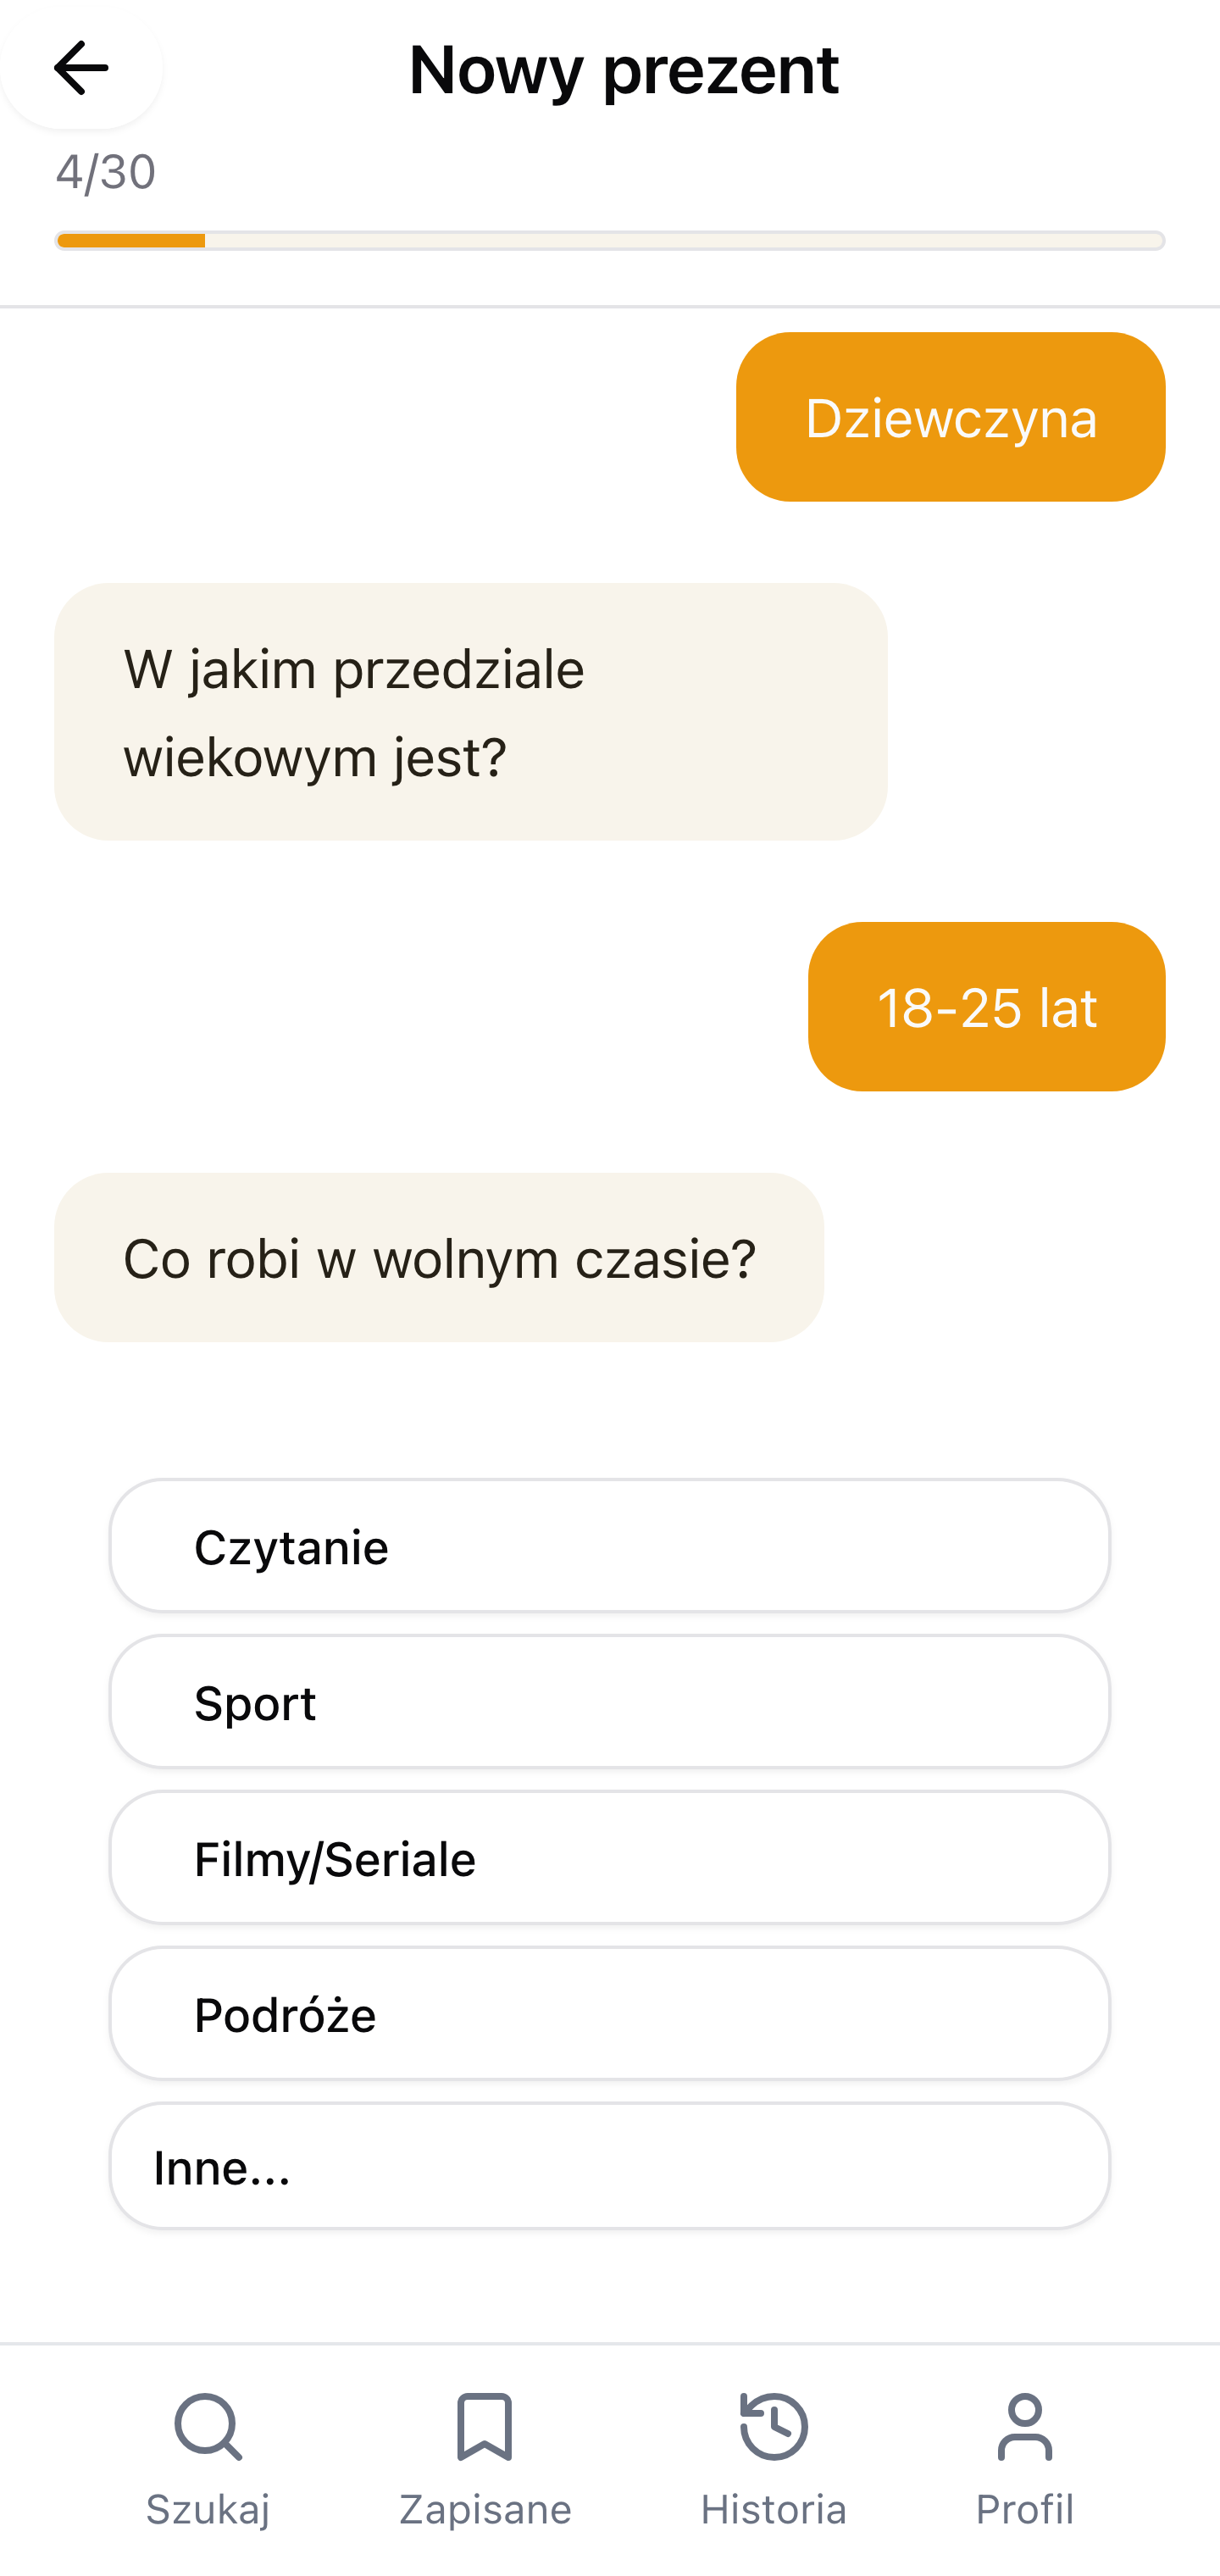
\includegraphics[width=\textwidth]{../designs/chat-id.png}
        \caption{Interfejs chatu z AI.}
        \label{fig:ui-chat}
    \end{subfigure}
    \hfill
    \begin{subfigure}[t]{0.48\textwidth}
        \centering
        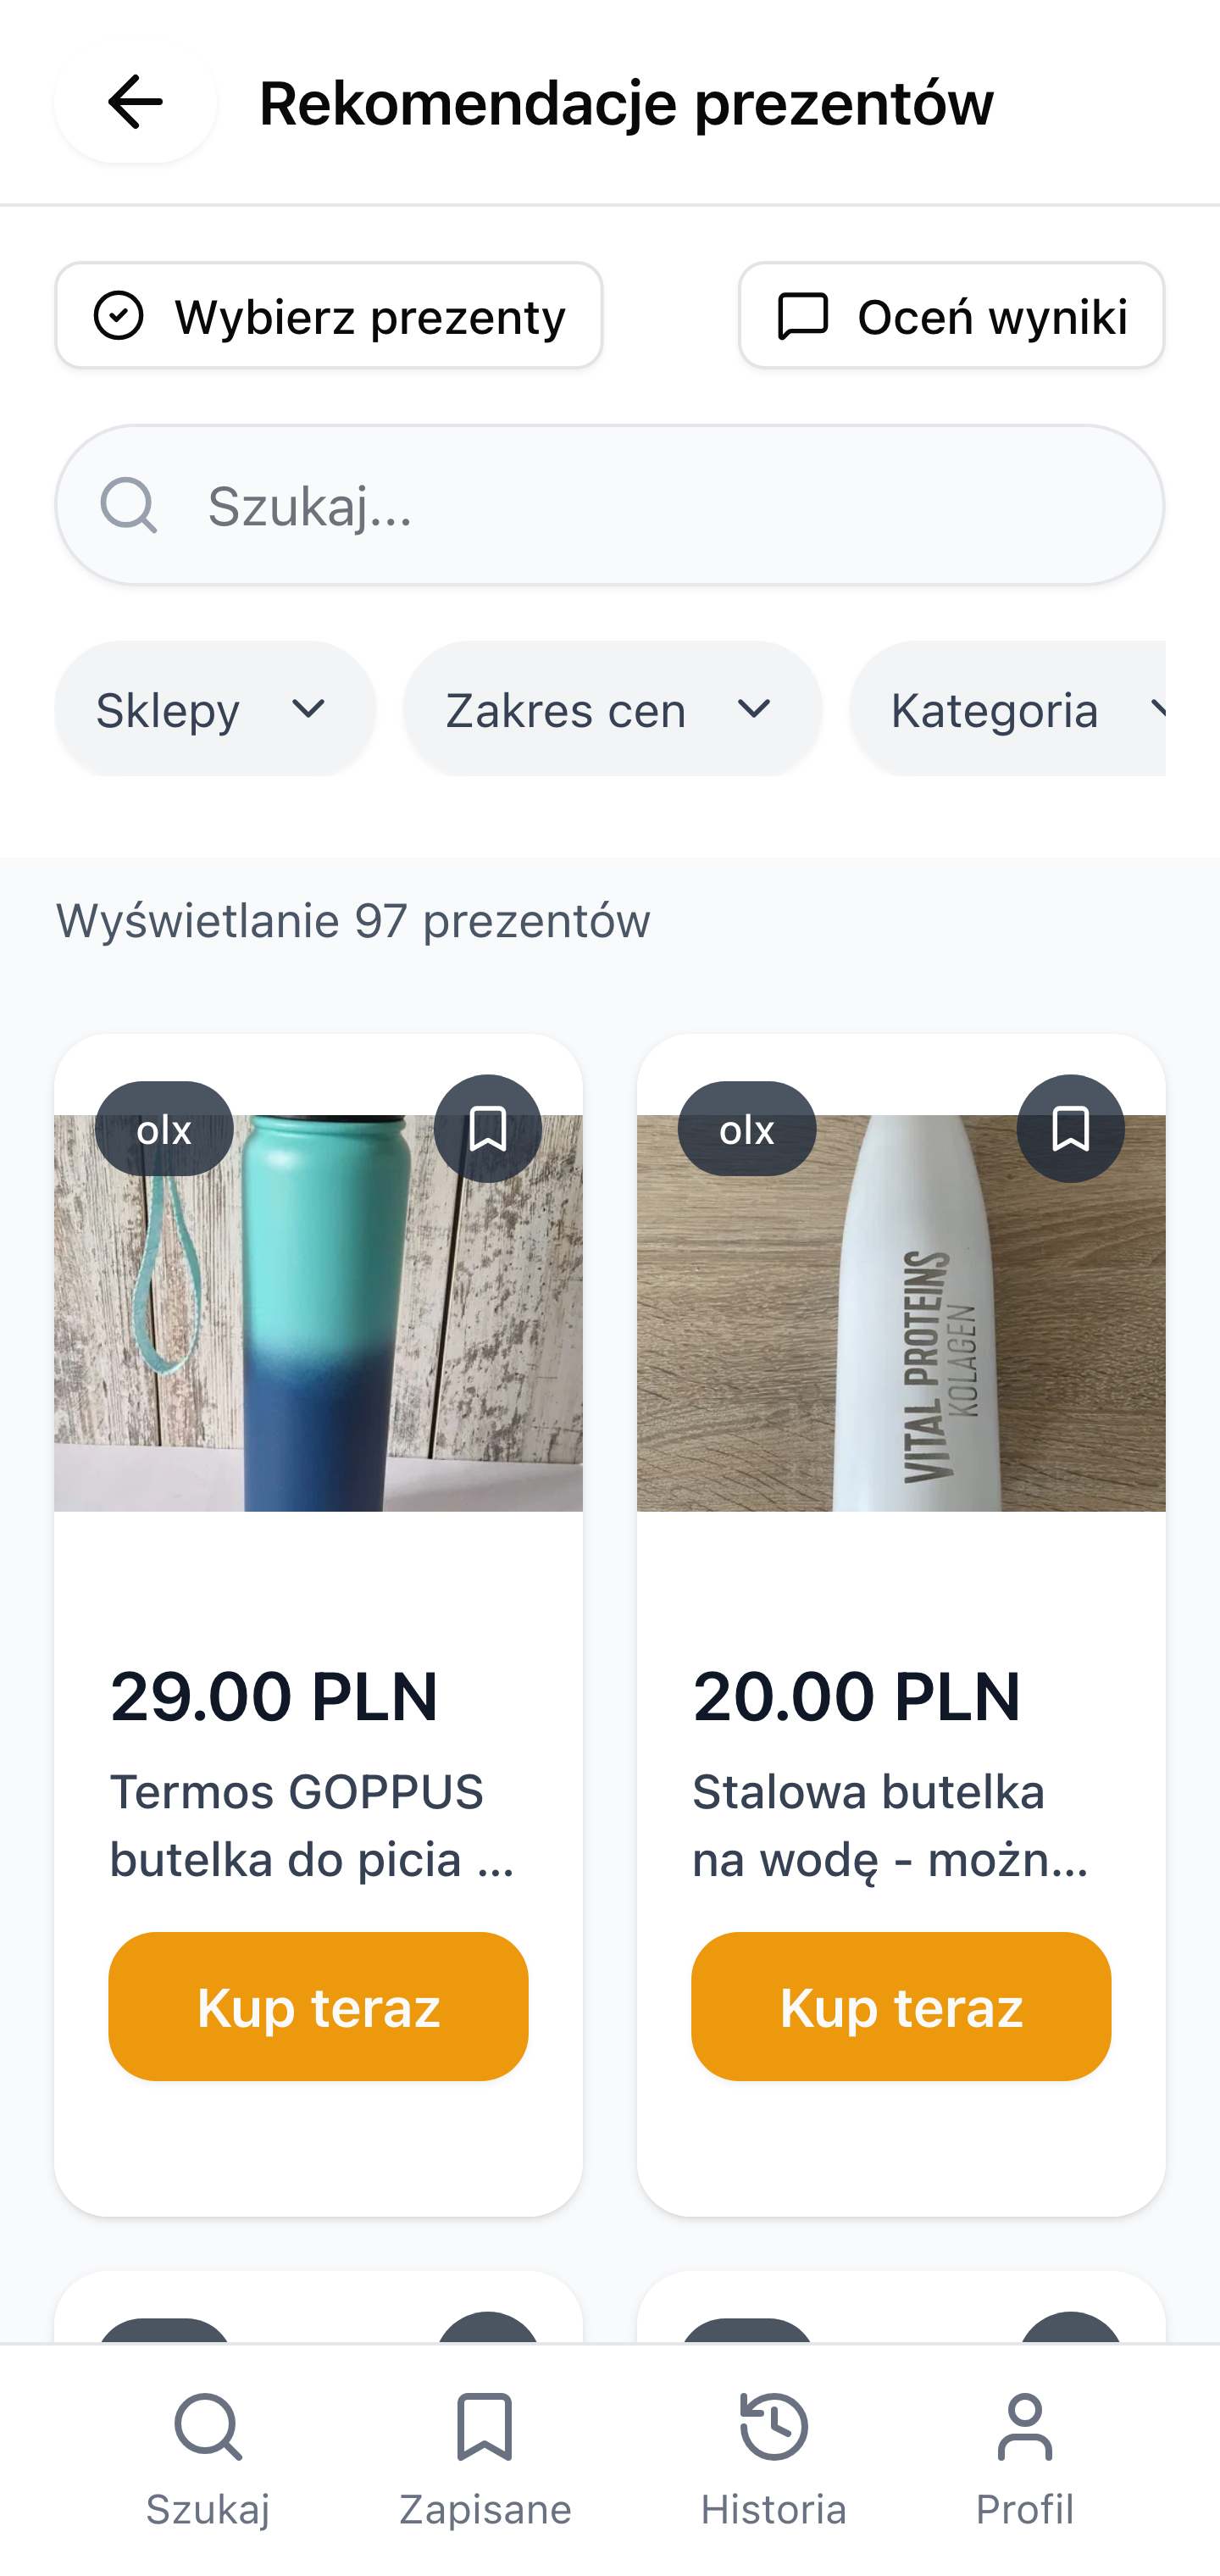
\includegraphics[width=\textwidth]{../designs/chat-id-results.png}
        \caption{Lista rekomendacji prezentów.}
        \label{fig:ui-results}
    \end{subfigure}
    \caption{Główny flow: wywiad z chatbotem i wynikowa lista rekomendacji.}
    \label{fig:ui-main-flow}
\end{figure}

\subsection{Krok 5: Nawigacja i zarządzanie}

Dolna belka nawigacyjna (widoczna na wszystkich ekranach po zalogowaniu) zapewnia szybki dostęp do czterech głównych sekcji aplikacji:

\textbf{a) Szukaj} – powrót do formularza nowego wyszukiwania.

\textbf{b) Zapisane} (Rysunek~\ref{fig:ui-saved}) – lista ulubionych produktów oznaczonych ikoną zakładki podczas przeglądania rekomendacji.

\textbf{c) Historia} (Rysunek~\ref{fig:ui-history}) – archiwum poprzednich sesji wyszukiwania z możliwością powrotu do wyników lub kontynuacji niedokończonej rozmowy.

\begin{figure}[H]
    \centering
    \begin{subfigure}[t]{0.48\textwidth}
        \centering
        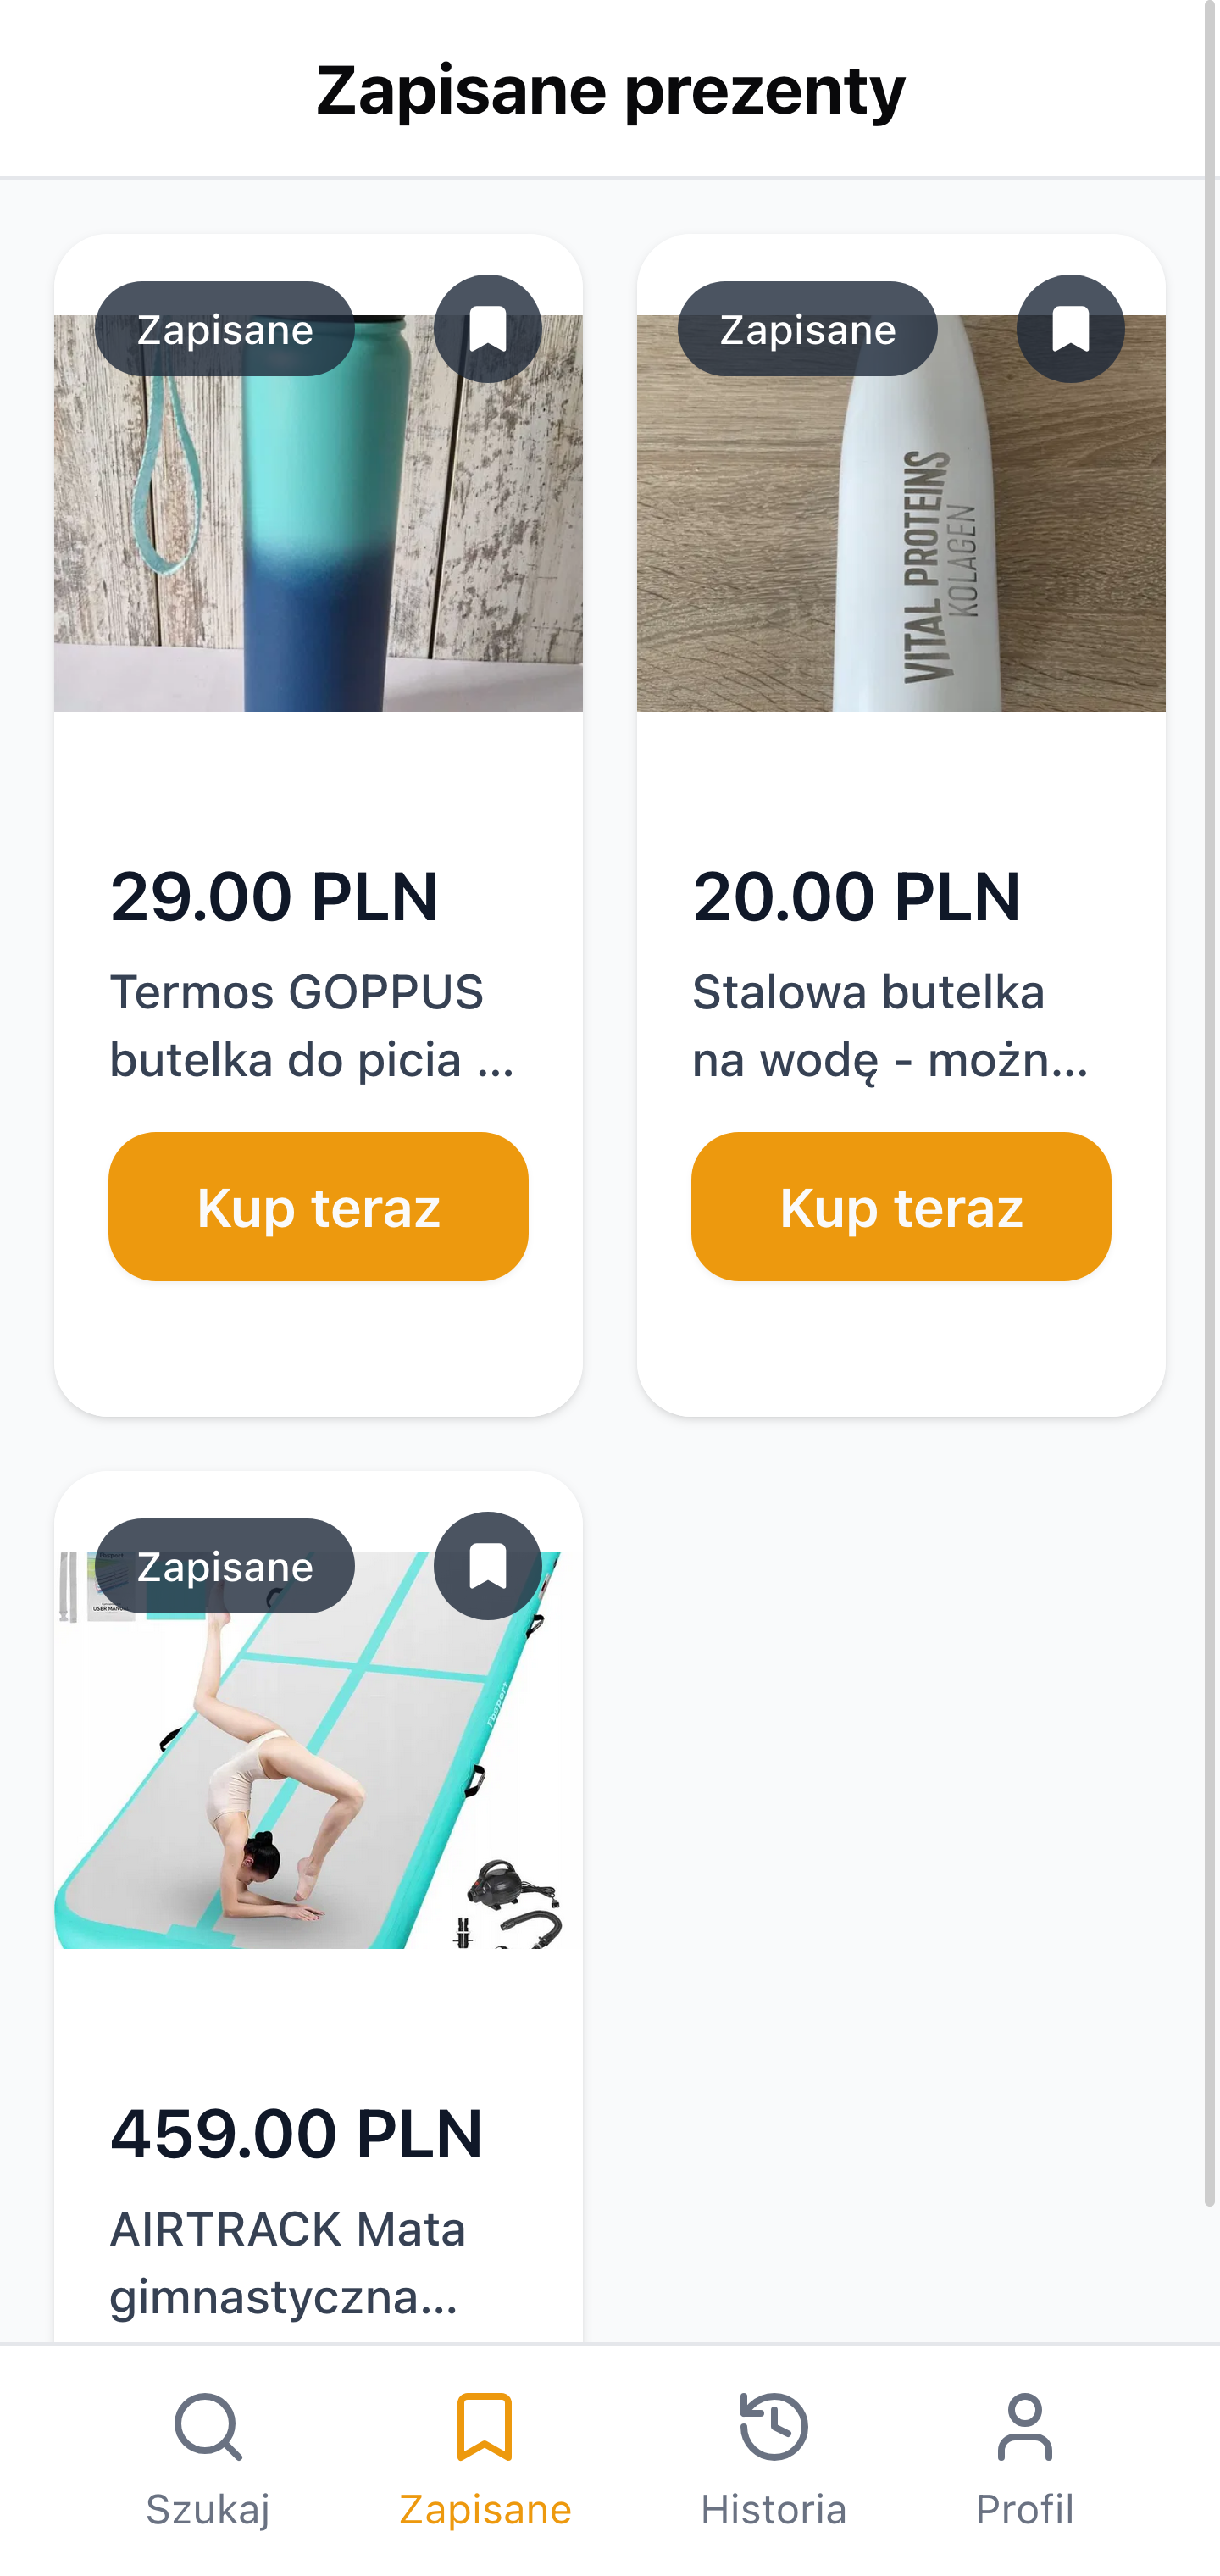
\includegraphics[width=\textwidth]{../designs/saved.png}
        \caption{Zapisane (ulubione) produkty.}
        \label{fig:ui-saved}
    \end{subfigure}
    \hfill
    \begin{subfigure}[t]{0.48\textwidth}
        \centering
        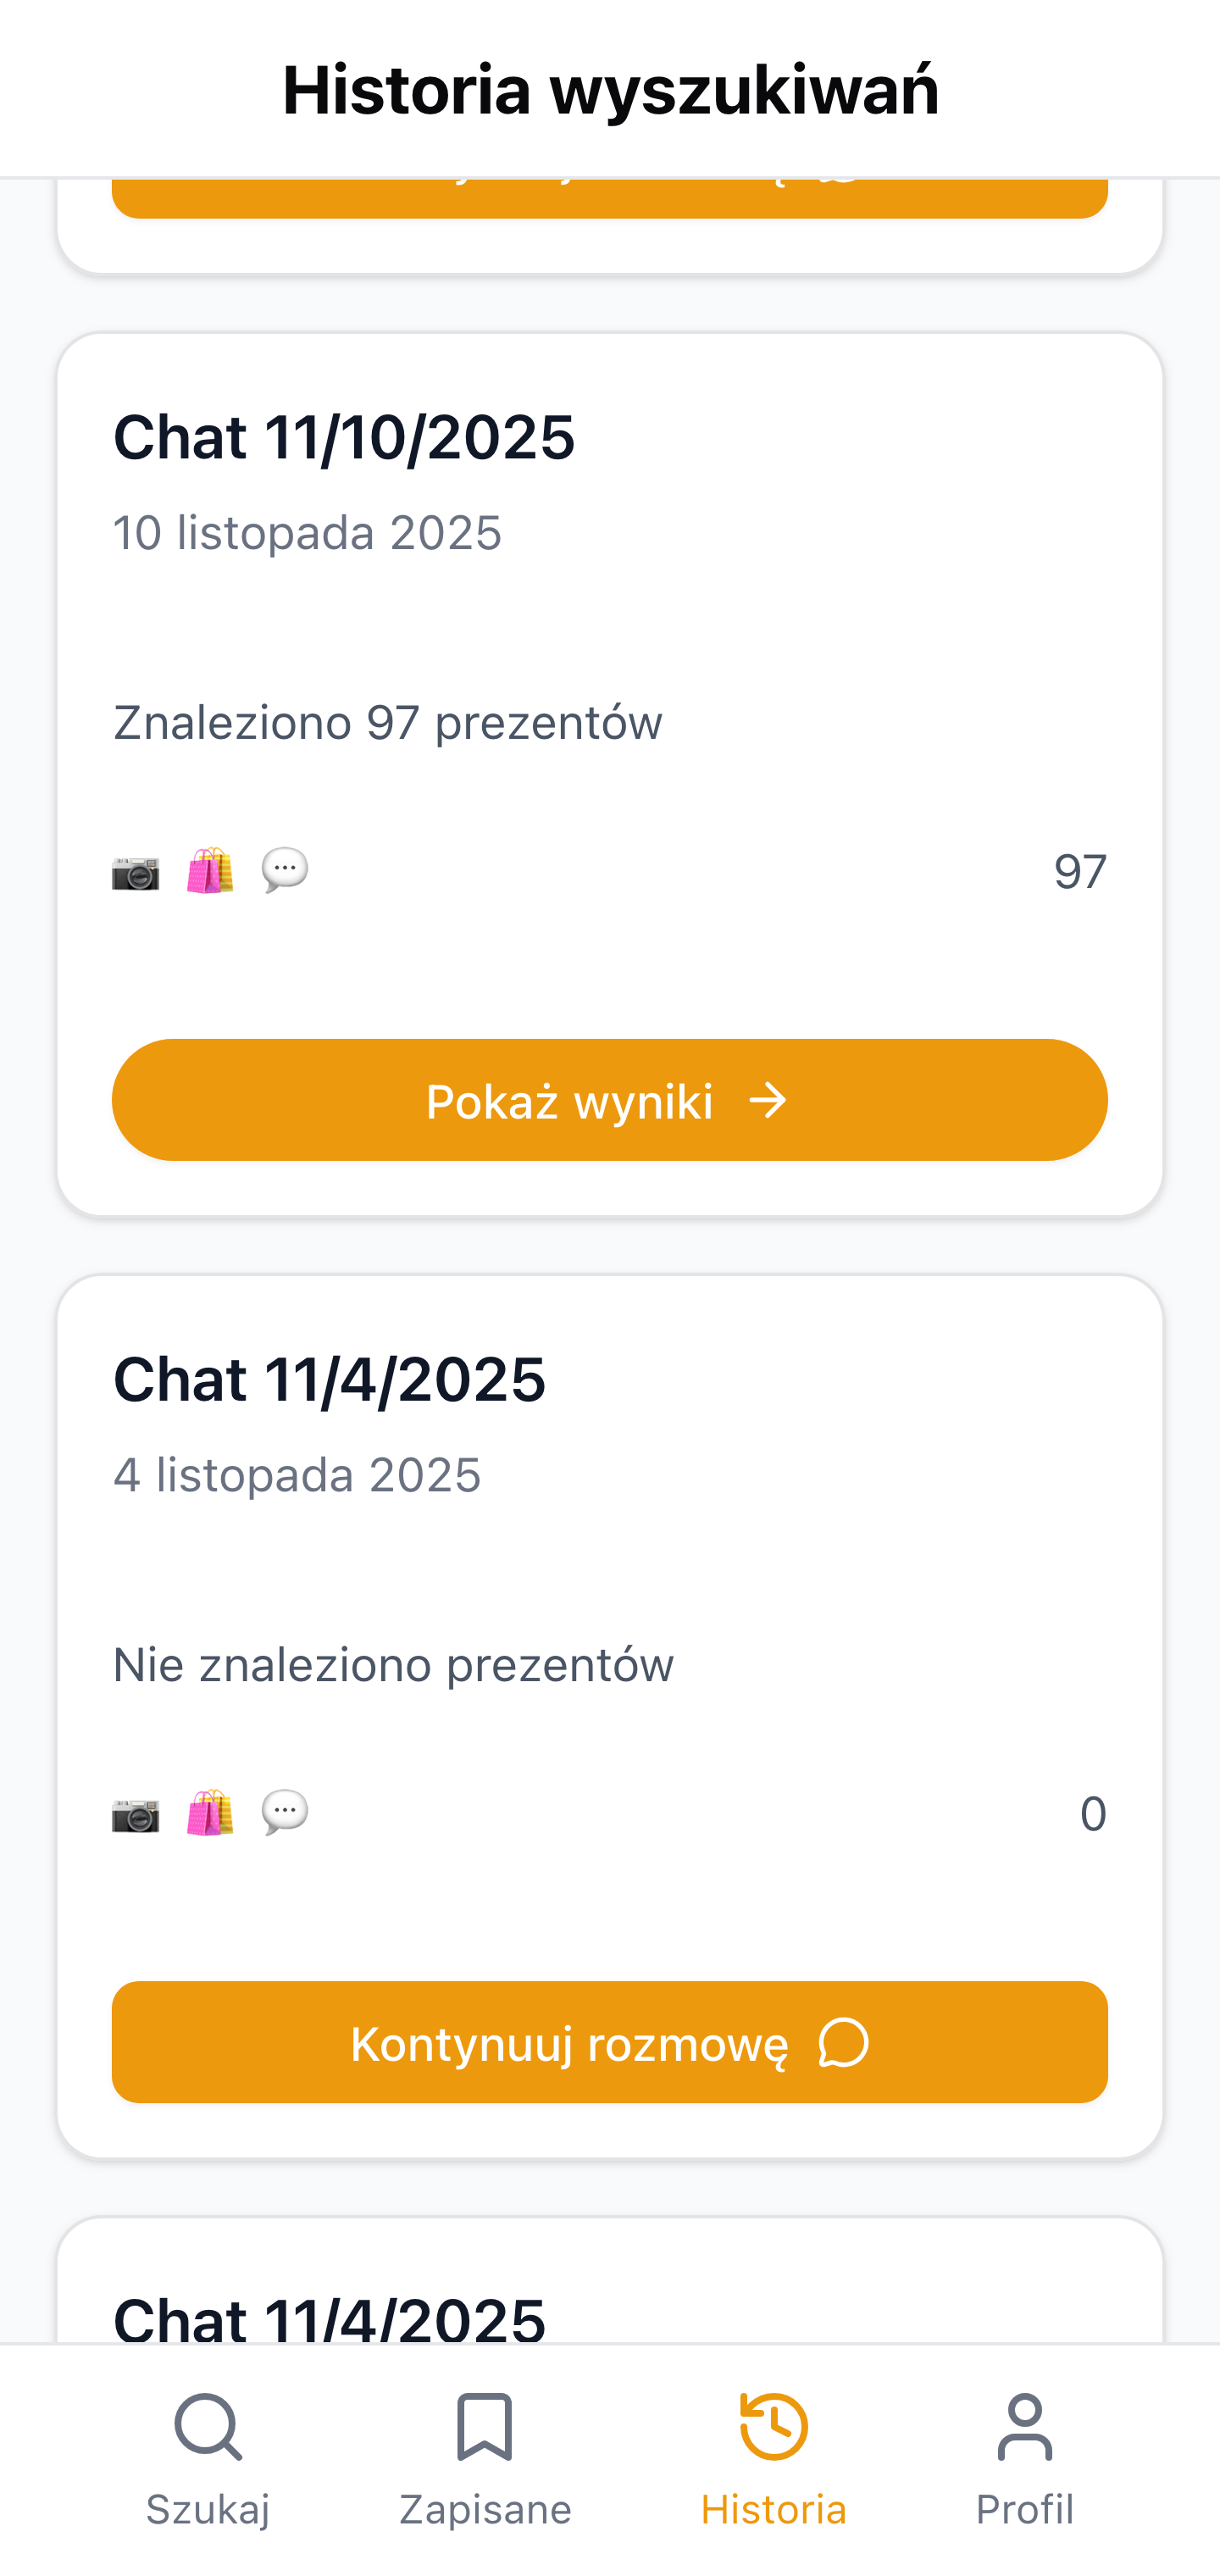
\includegraphics[width=\textwidth]{../designs/history.png}
        \caption{Historia sesji wyszukiwania.}
        \label{fig:ui-history}
    \end{subfigure}
    \caption{Zarządzanie danymi: zapisane produkty i historia sesji.}
    \label{fig:ui-management}
\end{figure}

\textbf{d) Profil} (Rysunek~\ref{fig:ui-profile}) – zarządzanie kontem użytkownika zawierające zdjęcie, dane, ustawienia konta oraz przycisk wylogowania. Administratorzy mają dodatkowo dostęp do panelu feedbacków.

\subsection{Panel administracyjny}

Użytkownicy z rolą administratora mają dostęp do panelu feedbacków (Rysunek~\ref{fig:ui-admin}), gdzie mogą przeglądać wszystkie opinie użytkowników pogrupowane według sesji. Panel wyświetla statystyki: łączną liczbę feedbacków, liczbę sesji z opiniami oraz średnią ocenę.

\begin{figure}[H]
    \centering
    \begin{subfigure}[t]{0.48\textwidth}
        \centering
        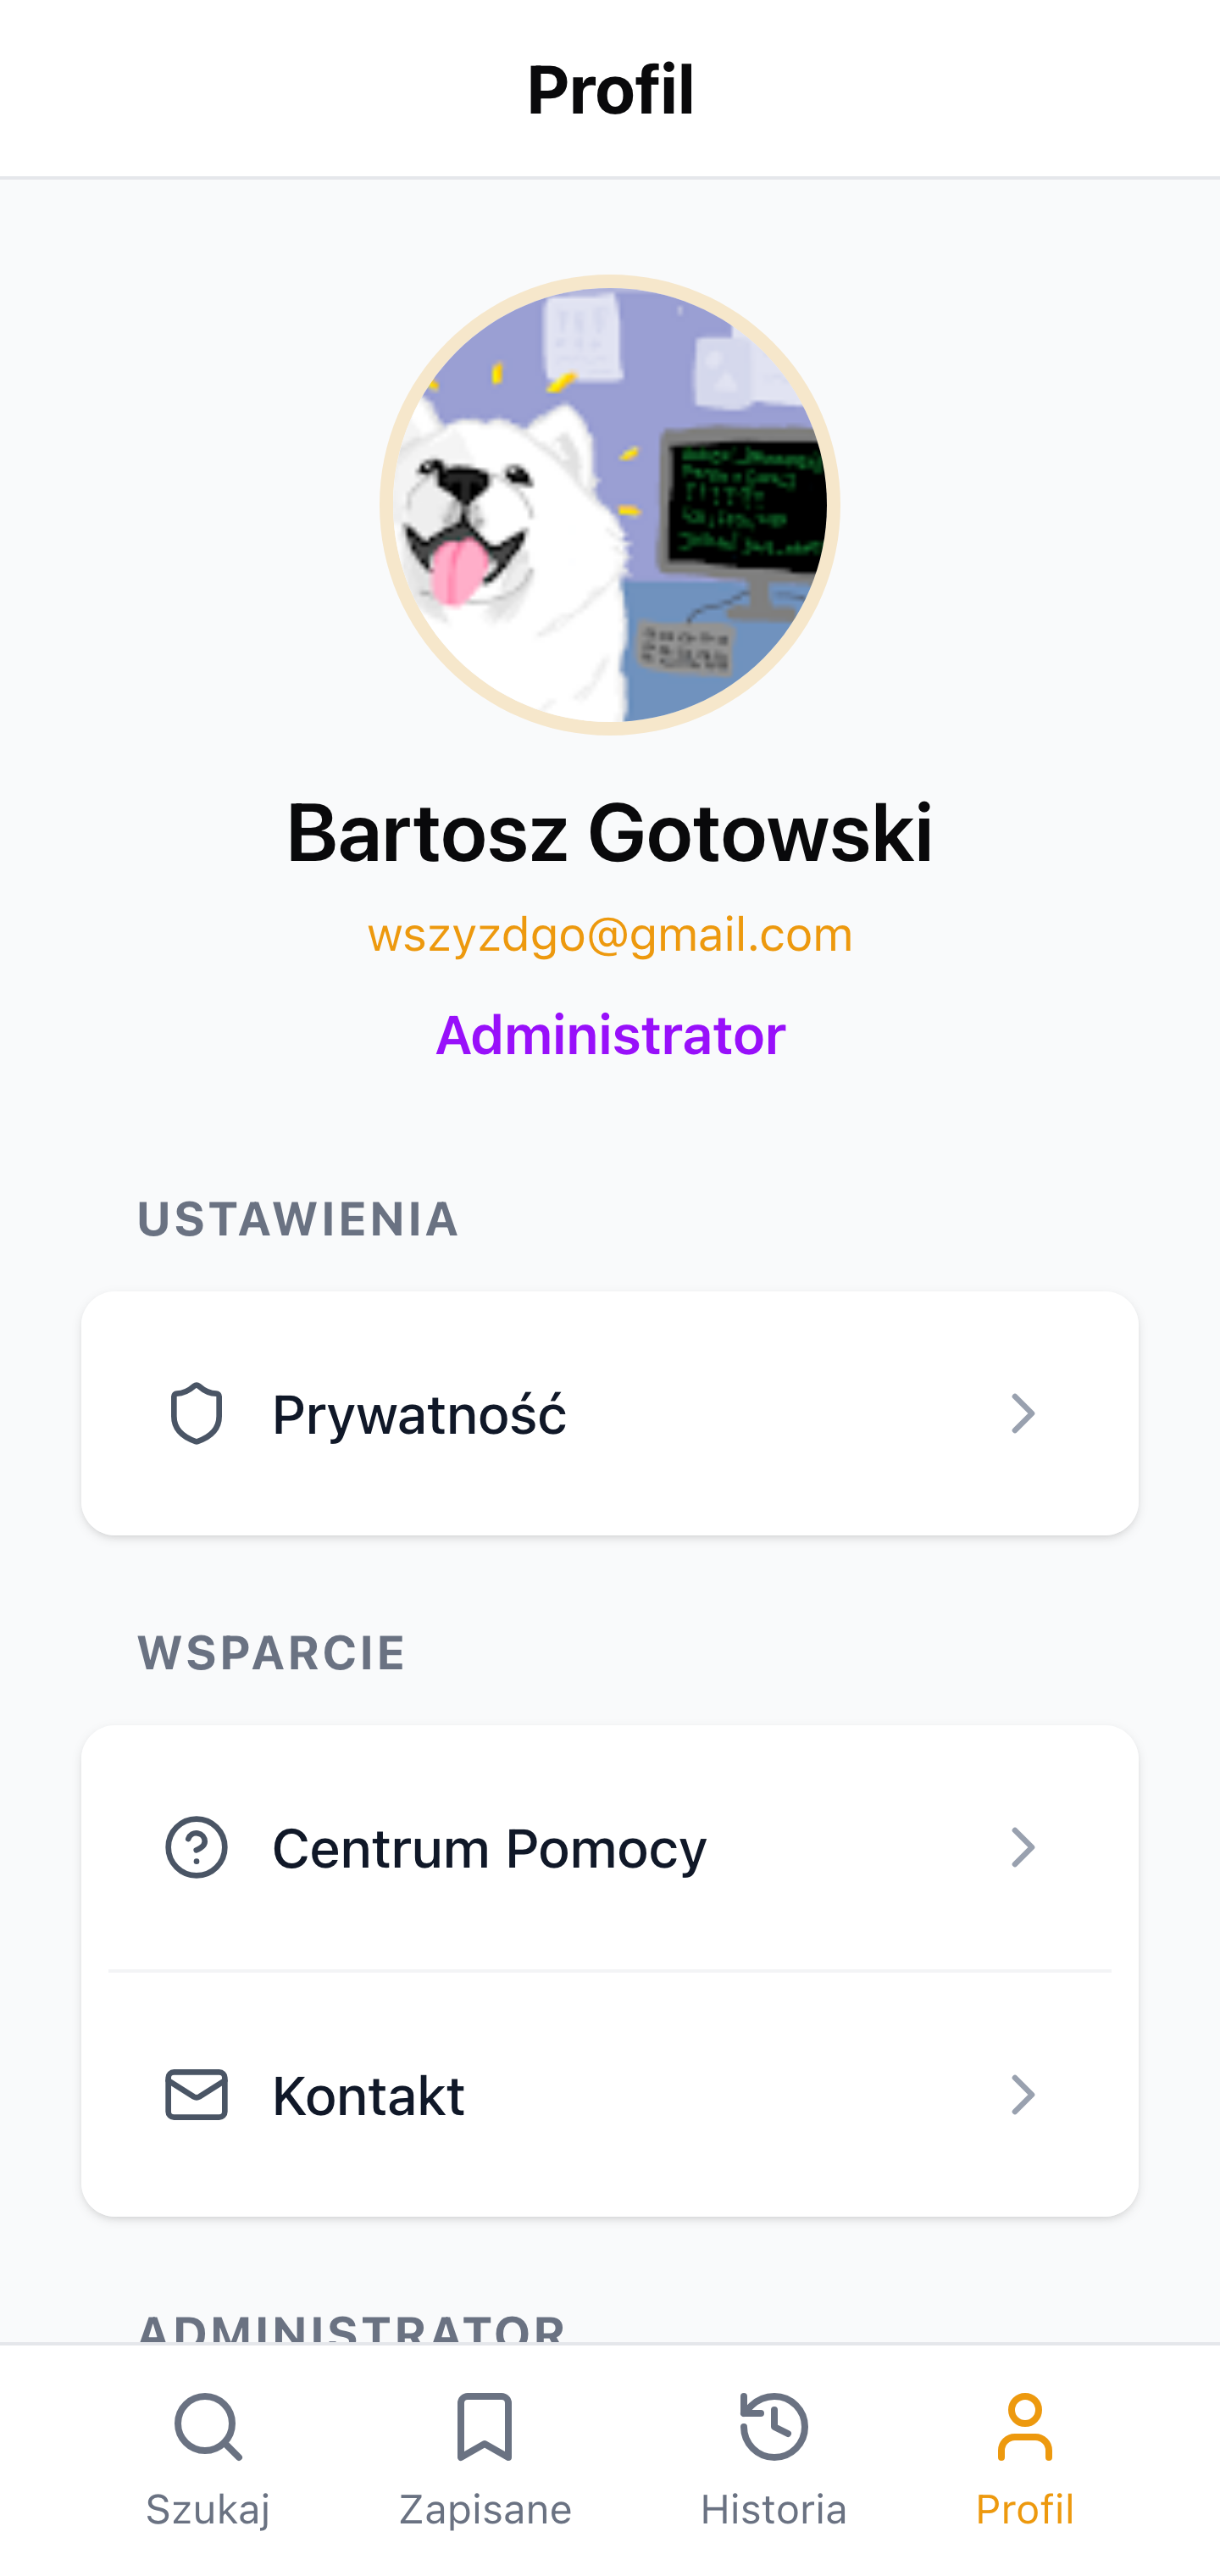
\includegraphics[width=\textwidth]{../designs/profile.png}
        \caption{Panel profilu użytkownika.}
        \label{fig:ui-profile}
    \end{subfigure}
    \hfill
    \begin{subfigure}[t]{0.48\textwidth}
        \centering
        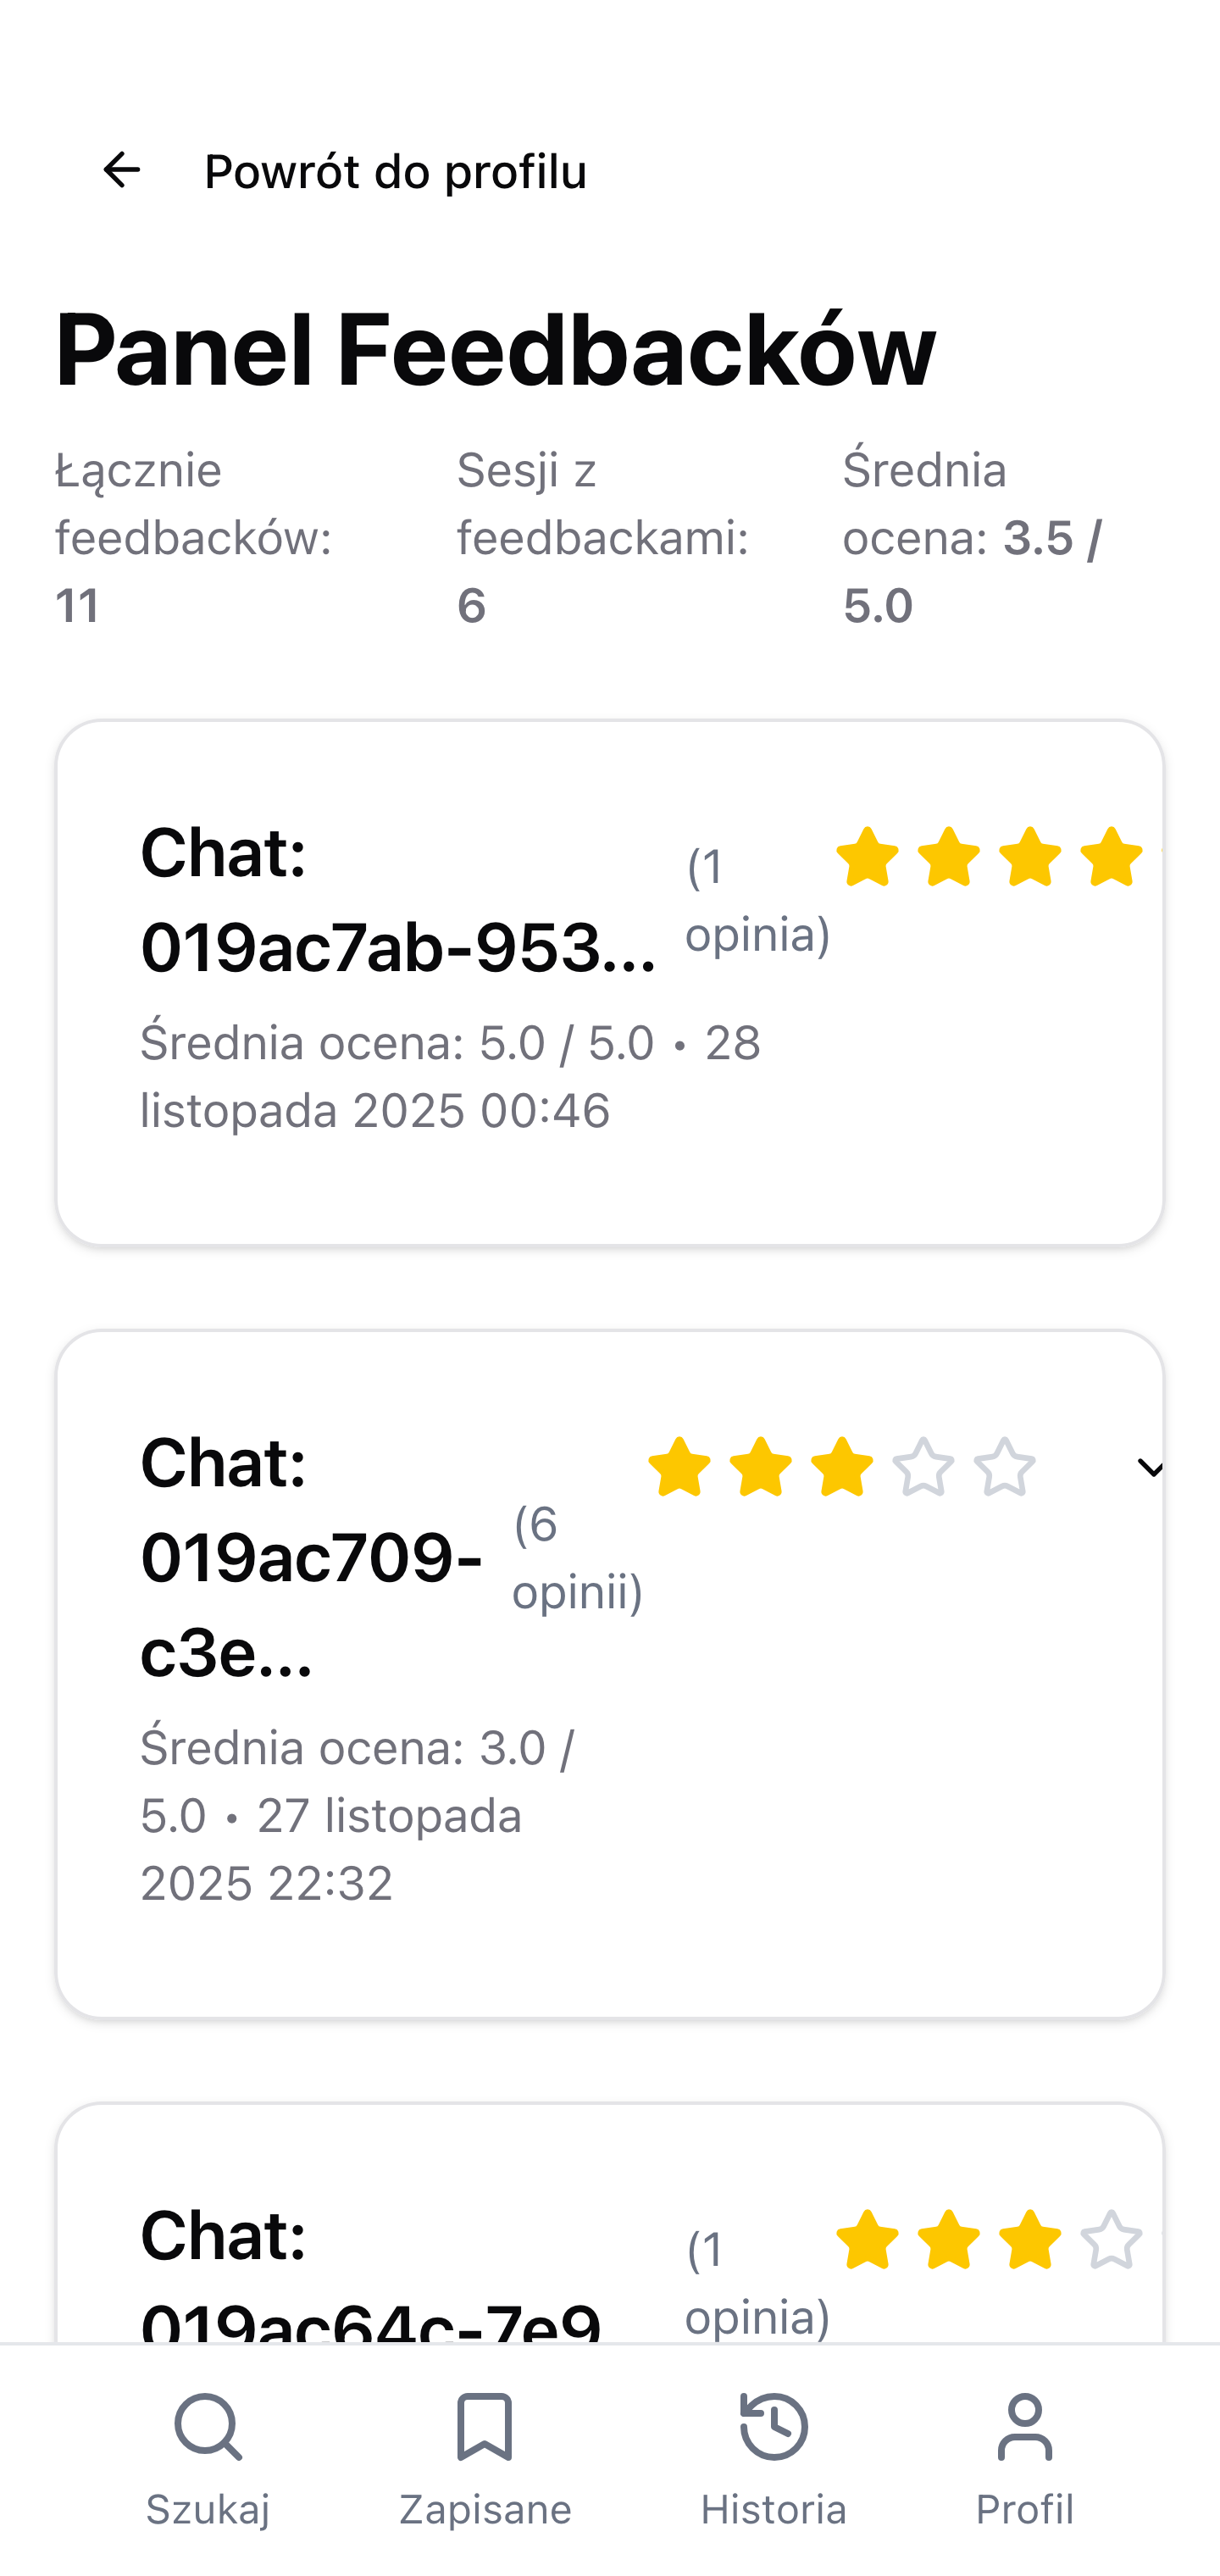
\includegraphics[width=\textwidth]{../designs/admin-feedback.png}
        \caption{Panel administracyjny – feedbacki.}
        \label{fig:ui-admin}
    \end{subfigure}
    \caption{Profil użytkownika i panel administracyjny.}
    \label{fig:ui-admin-profile}
\end{figure}

\section{Testy}

\subsection{Planowanie testów}
Strategia testowania zakładała kilka poziomów:
\begin{itemize}
    \item testy jednostkowe wybranych fragmentów logiki (np. parserów danych, prostych serwisów domenowych),
    \item testy integracyjne mikroserwisów (sprawdzenie poprawności kontraktów zdarzeń i komunikacji przez RabbitMQ),
    \item testy end-to-end podstawowego flow użytkownika (logowanie, wywiad, otrzymanie rekomendacji),
    \item testy wydajnościowe i odporności na błędy API (limity zapytań, czas odpowiedzi).
\end{itemize}
Do testów jednostkowych i integracyjnych wykorzystano ekosystem NestJS (Jest), natomiast testy E2E przeprowadzono z użyciem narzędzi takich jak Playwright lub Cypress (uruchamianych ręcznie dla kluczowych scenariuszy).

\subsection{Testy z użytkownikami}
Kluczowym elementem weryfikacji jakości systemu były beta-testy z udziałem rzeczywistych użytkowników. Zebrano opinie dotyczące trafności rekomendacji (oceny gwiazdkowe, komentarze tekstowe) oraz wrażeń z korzystania z interfejsu (czas oczekiwania, przejrzystość, intuicyjność). Dane te zostały wykorzystane zarówno w sekcji wyników, jak i przy planowaniu dalszego rozwoju (np. dodanie pamięci negatywnej, lepsze dopytywanie o budżet).

Jednym z głównych ryzyk, które miały wychwycić testy z użytkownikami, była odporność systemu na częściowe awarie integracji z serwisami e-commerce. W kilku sesjach celowo wyłączono jedną z instancji \texttt{Fetch Microservice} (np. odpowiedzialną za Allegro), aby sprawdzić, czy użytkownik nadal otrzyma sensowny zestaw propozycji z pozostałych źródeł i czy interfejs poprawnie komunikuje ograniczoną dostępność wyników.

W ramach testów szczególną uwagę zwrócono na scenariusz użytkownika szukającego prezentu dla fotografa–amatora. System zaproponował m.in. analogowy aparat z OLX, zestaw akcesoriów do aparatu oraz kurs fotografii online, a użytkownik ocenił całą sesję na 5/5 gwiazdek, podkreślając, że sam nie wpadłby na część tych pomysłów.

\section{Implementacja (opcja)}

\subsection{Algorytm Rerankingu z Weryfikacją (XAI)}
Kluczowym elementem systemu jest moduł rerankingu, który rozwiązuje problem "halucynacji" wyszukiwarek. Tradycyjne wyszukiwanie oparte na słowach kluczowych często zwraca wyniki nieadekwatne (np. akcesoria do konsoli zamiast konsoli). Zaimplementowany algorytm wykorzystuje model LLM (Gemini 2.5) do oceny semantycznej każdego produktu.
Dla każdej oferty model generuje:
\begin{itemize}
    \item Ocenę punktową (0-10) zgodności z profilem odbiorcy.
    \item Tekstowe uzasadnienie decyzji (np. "Odrzucono: Produkt to część zamienna, a nie gotowy prezent").
\end{itemize}
Pozwala to na odfiltrowanie ok. 40\% szumu informacyjnego.

Poniżej przedstawiono fragment systemu promptów definiującego kryteria oceny produktów:

Jak pokazano w Listingu~\ref{lst:reranking}, kryteria oceny produktów są zapisane w postaci czytelnego dla człowieka systemu promptów, który wymusza wyjaśnialne (XAI) decyzje modelu.

\begin{lstlisting}[caption={Fragment systemu promptów dla rerankingu produktów},label={lst:reranking}]
<criteria>
  <relevance priority="highest">
    Czy produkt odpowiada zainteresowaniom i hobby odbiorcy?
  </relevance>
  <lifestyle_fit priority="high">
    Czy produkt pasuje do stylu zycia i codziennej rutyny?
  </lifestyle_fit>
  <preferences priority="high">
    Czy produkt jest zgodny z preferencjami estetycznymi?
  </preferences>
  <occasion priority="medium">
    Czy produkt jest odpowiedni dla danej okazji?
  </occasion>
</criteria>

<scoring>
  1-3: Slabe dopasowanie - produkt nie pasuje do profilu
  4-6: Srednie dopasowanie - moze pasowac, ale nie jest idealny
  7-8: Dobre dopasowanie - produkt dobrze pasuje do profilu
  9-10: Doskonale dopasowanie - idealnie pasuje do profilu i okazji
  
  Wyniki ponizej 5 nie beda widoczne uzytkownikowi.
</scoring>
\end{lstlisting}

\subsection{Orkiestracja zdarzeń w architekturze CQRS}
Centralnym elementem systemu jest handler \texttt{StartProcessingCommand}, który orkiestruje rozpoczęcie całego procesu wyszukiwania prezentu. Po otrzymaniu żądania od użytkownika tworzy sesję chatu w bazie danych, a następnie równolegle publikuje dwa zdarzenia do kolejki RabbitMQ: jedno uruchamia analizę OSINT profili społecznościowych, drugie – wywiad z chatbotem.

Listing~\ref{lst:orchestration} przedstawia uproszczoną implementację tego handlera, podkreślając zasadę: najpierw utrwalenie sesji w bazie, dopiero później emisja zdarzeń do innych mikroserwisów.

\begin{lstlisting}[caption={Orkiestracja zdarzeń przy rozpoczęciu wyszukiwania prezentu},label={lst:orchestration}]
@CommandHandler(StartProcessingCommand)
export class StartProcessingCommandHandler {
  constructor(
    @Inject("STALKING_ANALYZE_REQUESTED_EVENT")
    private readonly stalkingEventBus: ClientProxy,
    @Inject("CHAT_START_INTERVIEW_EVENT")
    private readonly chatEventBus: ClientProxy,
    private readonly chatRepository: IChatRepository,
  ) {}

  async execute(command: StartProcessingCommand) {
    // 1. Najpierw tworzymy sesje w bazie danych
    const chat = await this.chatRepository.create({
      chatId: analyzeRequestedDto.chatId,
      chatName: `Chat ${new Date().toLocaleDateString()}`,
      userId,
    });

    // 2. Dopiero po utrwaleniu emitujemy zdarzenia rownolegle
    this.stalkingEventBus.emit(
      StalkingAnalyzeRequestedEvent.name, stalkingEvent
    );
    this.chatEventBus.emit(
      ChatStartInterviewEvent.name, interviewEvent
    );
  }
}
\end{lstlisting}

\subsection{Strukturyzacja rozmowy przez Tool Calling}
Moduł chatu wykorzystuje mechanizm \textit{tool calling} do wymuszenia strukturyzowanej odpowiedzi od modelu LLM. Zamiast swobodnego tekstu, AI musi wywołać jedno z trzech narzędzi: zadać pytanie z sugerowanymi odpowiedziami, zakończyć wywiad z wygenerowanym profilem, lub oznaczyć nieodpowiednie zapytanie.

Listing~\ref{lst:tools} pokazuje definicję tych narzędzi wraz z odpowiadającymi im schematami Zod, co zapewnia typowaną i przewidywalną współpracę pomiędzy LLM a resztą systemu.

\begin{lstlisting}[caption={Definicja narzędzi AI dla strukturyzacji wywiadu},label={lst:tools}]
export const tools = {
  ask_a_question_with_answer_suggestions: tool({
    description: "Zadaj pytanie z 4 sugerowanymi odpowiedziami",
    inputSchema: z.strictObject({
      question: z.string().min(1),
      potentialAnswers: potencialAnswersSchema,
    }),
  }),
  
  end_conversation: tool({
    description: "Zakoncz rozmowe z wygenerowanym profilem",
    inputSchema: z.object({
      output: endConversationOutputSchema, // profil odbiorcy
    }),
  }),
  
  flag_inappropriate_request: tool({
    description: "Oznacz nieetyczne lub nielegalne zapytanie",
    inputSchema: z.object({
      reason: z.string(),
    }),
  }),
} as const;
\end{lstlisting}

Dzięki temu podejściu każda odpowiedź AI jest typowana i walidowana schematem Zod, co eliminuje problemy z parsowaniem i zapewnia spójność przepływu danych między mikroserwisami.

\subsection{Inżynieria promptów (Prompt Engineering)}

Jednym z najważniejszych aspektów implementacji systemu AI Present Finder była iteracyjna optymalizacja promptów -- instrukcji przekazywanych modelom językowym. W ciągu 80 dni rozwoju projektu (wrzesień--listopad 2025) przeprowadzono ponad 25 iteracji promptów, co przełożyło się na znaczącą poprawę jakości generowanych rekomendacji.

\paragraph{Ewolucja promptów.}
System wykorzystuje 5 specjalizowanych promptów, z których każdy przeszedł własną ścieżkę optymalizacji:

\begin{table}[h]
\centering
\begin{tabular}{|p{0.22\textwidth}|p{0.12\textwidth}|p{0.55\textwidth}|}
\hline
\textbf{Prompt} & \textbf{Iteracje} & \textbf{Kluczowe zmiany} \\
\hline
Chat (wywiad) & 12 & Format XML, min. 30 pytań, 3. osoba, podejście produktowe \\
\hline
Refinement & 2 & Doprecyzowanie po wyborze produktów (3--5 pytań) \\
\hline
Stalking (OSINT) & 3 & Ekstrakcja faktów z profili społecznościowych \\
\hline
Gift Ideas & 5 & Generowanie zapytań dla 5 platform, max 5 wyrazów \\
\hline
Reranking & 4 & Scoring 1--10, filtrowanie $\geq$5, batching \\
\hline
\end{tabular}
\caption{Przegląd promptów i liczba iteracji w projekcie}
\end{table}

\paragraph{Kluczowe problemy i rozwiązania.}
Podczas rozwoju systemu zidentyfikowano i rozwiązano szereg problemów związanych z zachowaniem modeli LLM:

\begin{itemize}
    \item \textbf{Za krótkie rozmowy:} Początkowy prompt generował tylko 10 pytań, co dawało niewystarczające dane. Rozwiązanie: dodanie licznika pytań i wymuszenie minimum 30 pytań przed zakończeniem wywiadu.
    \item \textbf{Pytania w 2. osobie:} Model pytał ,,Czy lubisz gotować?'' zamiast ,,Czy ON/ONA lubi gotować?''. Rozwiązanie: explicite reguła w prompcie wymuszająca 3. osobę.
    \item \textbf{Zbyt abstrakcyjne pytania:} Pytania typu ,,Jaki styl preferuje?'' nie prowadziły do konkretnych kategorii produktów. Rozwiązanie: podejście produktowe -- ,,Czy ma dobre słuchawki?'' zamiast ,,Jaki rodzaj muzyki lubi?''.
    \item \textbf{Brak różnorodności:} Model zawsze zaczynał od pracy zawodowej. Rozwiązanie: lista 16 obszarów eksploracji z wymogiem pokrycia min. 5 różnych.
    \item \textbf{Drążenie po ,,nie wiem'':} Model kontynuował ten sam wątek mimo braku wiedzy użytkownika. Rozwiązanie: reguła natychmiastowej zmiany obszaru po odpowiedzi ,,nie wiem''.
    \item \textbf{Brakujące tool calls:} Model czasami odpowiadał tekstem zamiast wywołać narzędzie. Rozwiązanie: mechanizm auto-retry z przypomnieniem w kolejnej wiadomości.
\end{itemize}

\paragraph{Struktura prompta wywiadu.}
Największy prompt (Chat) liczy ponad 700 linii i wykorzystuje format XML dla lepszej czytelności przez model. Listing~\ref{lst:prompt-structure} przedstawia uproszczoną strukturę tego prompta.

\begin{lstlisting}[caption={Struktura prompta wywiadu z użytkownikiem (uproszczony)},label={lst:prompt-structure}]
<system>
  <role>Jestes Doradca Prezentowym - prowadzisz rozmowe 
        (15-30 pytan) aby poznac obdarowywanego.</role>
  
  <context>
    <occasion>${occasion}</occasion>
    <conversation_progress>
      <current_question_number>${questionCount}</current_question_number>
      <status>MUSISZ ZADAC PRZYNAJMNIEJ ${30 - questionCount} 
              PYTAN WIECEJ!!!</status>
    </conversation_progress>
  </context>
  
  <critical_rules>
    <rule id="1">JEDNO pytanie na raz, PROSTE, konkretne</rule>
    <rule id="2">TRZECIA osoba (on/ona) - NIGDY druga osoba</rule>
    <rule id="3">Pytaj PRODUKTOWO, nie abstrakcyjnie</rule>
    <rule id="5">Eksploruj MINIMUM 5 ROZNYCH obszarow zycia</rule>
    <rule id="6">"Nie wiem" = NATYCHMIAST zmien watek</rule>
  </critical_rules>
  
  <exploration_leads>
    PRACA, DOM, HOBBY, KULINARIA, TECHNOLOGIA, ZDROWIE,
    PODROZE, MUZYKA, ZWIERZETA, SZTUKA, GAMING, FOTOGRAFIA...
  </exploration_leads>
  
  <tools>
    <tool name="ask_a_question_with_answer_suggestions"/>
    <tool name="end_conversation"/>
    <tool name="flag_inappropriate_request"/>
  </tools>
</system>
\end{lstlisting}

\paragraph{Wyniki optymalizacji.}
Iteracyjne doskonalenie promptów przyniosło wymierne rezultaty:
\begin{itemize}
    \item Liczba pytań w wywiadzie: 10 $\rightarrow$ 30 (3$\times$ więcej danych o odbiorcy),
    \item Obszary eksploracji: 6 $\rightarrow$ 16+ kategorii życia,
    \item Sukces tool calls: $\sim$60\% $\rightarrow$ $\sim$95\% (dzięki auto-retry),
    \item Trafność pierwszej rekomendacji: wzrost do 64\% (First Hit Accuracy).
\end{itemize}

Kluczowym wnioskiem z procesu prompt engineeringu jest znaczenie \textbf{konkretnych przykładów} i \textbf{explicite zakazów} w instrukcjach. Model lepiej rozumie ,,NIE pytaj o budżet'' niż ,,skup się na zainteresowaniach''. Podobnie, podanie 2--3 przykładowych rozmów w prompcie drastycznie poprawia jakość generowanych pytań.

\subsection{Równoległa Agregacja Ofert}
Ze względu na limity API i czas odpowiedzi serwisów e-commerce, zaimplementowano mechanizm równoległego pobierania danych. \texttt{Fetch Microservice} może być uruchamiany w wielu instancjach, z których każda obsługuje innego dostawcę (OLX, Allegro, Amazon). Wyniki są asynchronicznie przesyłane do głównego strumienia zdarzeń, co pozwala na prezentowanie pierwszych ofert użytkownikowi bez czekania na zakończenie przeszukiwania wszystkich źródeł.

\section{Wyniki i analiza badań}

System został poddany testom w środowisku produkcyjnym (pilotaż, listopad 2025). W analizie wzięto pod uwagę 36 pełnych sesji zakupowych.

\subsection{Efektywność czasowa}
Średni czas potrzebny na znalezienie prezentu został zredukowany z rynkowej średniej 15 godzin (rocznie) do \textbf{7 minut i 44 sekund} na sesję. W tym czasie system przeprowadza wywiad z użytkownikiem, analizuje profil społecznościowy i przeszukuje cztery platformy e-commerce.

\subsection{Jakość rekomendacji}
\begin{itemize}
    \item \textbf{Trafność (First Hit Accuracy):} 64\% użytkowników uznało pierwszą propozycję za trafną.
    \item \textbf{Redukcja szumu:} Moduł rerankingu odrzuca średnio 40\% ofert jako nietrafione lub niskiej jakości (np. części zamienne zamiast produktów).
    \item \textbf{Satysfakcja użytkowników:} Średnia ocena 3.5/5.0. Użytkownicy docenili trafność pomysłów, ale wskazywali na problem polecania rzeczy, które obdarowywany już posiada (brak "pamięci negatywnej" w MVP).
\end{itemize}

\subsection{Przykłady rerankingu AI (Explainable AI)}

Moduł rerankingu wykorzystuje model Gemini 2.5 Flash Lite do oceny każdego produktu w skali 1--10 wraz z uzasadnieniem. Na podstawie danych z produkcji (2512 produktów, 2380 z oceną) przeanalizowano rozkład ocen:

\begin{table}[H]
\centering
\small
\begin{tabular}{|l|r|r|}
\hline
\textbf{Zakres ocen} & \textbf{Liczba produktów} & \textbf{Procent} \\
\hline
Ocena 1--3 (odfiltrowane) & 391 & 16\% \\
Ocena 4--5 (słabe dopasowanie) & 267 & 11\% \\
Ocena 6--7 (dobre dopasowanie) & 779 & 33\% \\
Ocena 8--9 (bardzo dobre) & 899 & 38\% \\
Ocena 10 (idealne) & 44 & 2\% \\
\hline
\textbf{Średnia ocena} & \multicolumn{2}{c|}{\textbf{6.38/10}} \\
\hline
\end{tabular}
\caption{Rozkład ocen rerankingu AI (dane produkcyjne, grudzień 2025)}
\end{table}

\subsubsection*{Produkty z oceną 10 (idealne dopasowanie)}
\begin{table}[H]
\centering
\small
\begin{tabular}{|p{0.32\textwidth}|p{0.08\textwidth}|p{0.05\textwidth}|p{0.45\textwidth}|}
\hline
\textbf{Tytuł} & \textbf{Cena} & \textbf{Ocena} & \textbf{Uzasadnienie AI} \\
\hline
Herman Miller Aeron C full pakiet & 3 800 zł & 10 & Najwyższej klasy fotel biurowy, znany z niezrównanej ergonomii i komfortu, idealnie wpisuje się w potrzeby osoby ceniącej wygodę siedzenia. \\
\hline
Fotel gamingowy Diablo X-Horn & 500 zł & 10 & Wygodny i stylowy fotel gamingowy, zapewniający najwyższy komfort i funkcjonalność. Idealnie pasuje do potrzeb odbiorcy szukającego ergonomicznego fotela. \\
\hline
Fotel Secret Lab jak NOWY + akcesoria & 1 599 zł & 10 & Fotel gamingowy Secret Lab jak nowy, z dodatkowymi akcesoriami i w świetnej cenie, jest idealnym prezentem. \\
\hline
\end{tabular}
\end{table}

\subsubsection*{Produkty z oceną 1 (odfiltrowane jako niepasujące)}
\begin{table}[H]
\centering
\small
\begin{tabular}{|p{0.32\textwidth}|p{0.08\textwidth}|p{0.05\textwidth}|p{0.45\textwidth}|}
\hline
\textbf{Tytuł} & \textbf{Cena} & \textbf{Ocena} & \textbf{Uzasadnienie AI} \\
\hline
Duża kuchenka dla dzieci mega zestaw & 189 zł & 1 & Duża kuchenka dla dzieci jest całkowicie nieodpowiednia dla odbiorcy w wieku 18--25 lat i nie ma związku z jego zainteresowaniami. \\
\hline
Koci Domek Gabi z figurkami & 249 zł & 1 & Produkt jest zabawką przeznaczoną dla małych dzieci, co całkowicie mija się z zainteresowaniami i wiekiem odbiorcy. \\
\hline
Kuchnia drewniana IKEA dla dzieci & 120 zł & 1 & Zabawka przeznaczona dla dzieci 1--3 lata, całkowicie nieodpowiednia dla dorosłego odbiorcy. \\
\hline
\end{tabular}
\end{table}

Reranking skutecznie eliminuje produkty nietrafione kontekstowo (zabawki dla dzieci przy szukaniu prezentów dla dorosłych) i przyznaje wysokie oceny produktom dokładnie odpowiadającym profilowi odbiorcy. System odfiltrował 27\% produktów (oceny 1--3) jako niepasujące.

\subsection{Feedback użytkowników}

W ramach testów pilotażowych zebrano 11 opinii od użytkowników. Poniżej przedstawiono reprezentatywne cytaty:

\subsubsection*{Opinie pozytywne}
\begin{itemize}
    \item \textit{"Trafiony w sedno jak na tak niedługą i przyjemną rozmowę."} (Ocena: 5/5)
    \item \textit{"Szybko, sprawnie, widać że system próbuje zrozumieć kontekst. Propozycje były sensowne i w budżecie."} (Ocena: 4/5)
    \item \textit{"Świetny pomysł na aplikację! Wyniki były zaskakująco trafne."} (Ocena: 4/5)
\end{itemize}

\subsubsection*{Opinie krytyczne i sugestie}
\begin{itemize}
    \item \textit{"Większość prezentów miała wspólne cechy z prezentami które były kupione w przeszłości — system polecał rzeczy, które osoba już ma."} (Ocena: 3/5) — wskazuje na potrzebę "pamięci negatywnej".
    \item \textit{"OLX przytłaczające, brak wyników z Allegro. Rozmowa była zbyt długa."} (Ocena: 2/5) — sugestia balansowania źródeł i skrócenia wywiadu.
\end{itemize}

\noindent Główne wnioski z feedbacku:
\begin{enumerate}
    \item 64\% użytkowników uznało pierwszy wynik za trafny
    \item Najczęstszy problem: polecanie przedmiotów już posiadanych przez obdarowywanego
    \item Użytkownicy docenili szybkość działania i naturalność konwersacji
\end{enumerate}

\subsection{Stabilność}
System osiągnął 100\% dostępności (uptime) podczas testów, przy minimalnym zużyciu zasobów (<800MB RAM dla całego klastra), co potwierdza poprawność założeń architektonicznych.

\end{document}